\documentclass{tufte-book} % Use the tufte-book class which in turn uses the tufte-common class

\hypersetup{colorlinks} % Comment this line if you don't wish to have colored links
\usepackage{microtype} % Improves character and word spacing
\usepackage{booktabs} % Better horizontal rules in tables

\usepackage{texnames}
\usepackage{epigraph}
\usepackage{amsmath,amsfonts,amssymb}
\usepackage{bm,bbm}
\usepackage[caption=false]{subfig}
\usepackage{siunitx}

\usepackage{listings}
\lstset{language=R}
\lstset{basicstyle=\footnotesize\ttfamily,breaklines=true}
\lstset{framextopmargin=50pt,frame=bottomline}

\usepackage{graphicx} % Needed to insert images into the document
\graphicspath{{./Figures/}} % Sets the default location of pictures
\setkeys{Gin}{width=\linewidth,totalheight=\textheight,keepaspectratio} % Improves figure scaling

\usepackage{fancyvrb} % Allows customization of verbatim environments
\fvset{fontsize=\normalsize} % The font size of all verbatim text can be changed here

\newcommand{\hangp}[1]{\makebox[0pt][r]{(}#1\makebox[0pt][l]{)}} % New command to create parentheses around text in tables which take up no horizontal space - this improves column spacing
\newcommand{\hangstar}{\makebox[0pt][l]{*}} % New command to create asterisks in tables which take up no horizontal space - this improves column spacing

\newcommand{\E}{\operatorname{E}}
\newcommand{\Var}{\operatorname{Var}}
\newcommand{\CV}{\operatorname{CV}}

\usepackage{xspace} % Used for printing a trailing space better than using a tilde (~) using the \xspace command

\newcommand{\monthyear}{\ifcase\month\or January\or February\or March\or April\or May\or June\or July\or August\or September\or October\or November\or December\fi\space\number\year} % A command to print the current month and year

\newcommand{\openepigraph}[2]{ % This block sets up a command for printing an epigraph with 2 arguments - the quote and the author
\begin{fullwidth}
\sffamily\large
\begin{doublespace}
\noindent\allcaps{#1}\\ % The quote
\noindent\allcaps{#2} % The author
\end{doublespace}
\end{fullwidth}
}

\setcounter{secnumdepth}{2}
\setcounter{tocdepth}{2}

\newcommand{\blankpage}{\newpage\hbox{}\thispagestyle{empty}\newpage} % Command to insert a blank page

\usepackage{makeidx} % Used to generate the index
\makeindex % Generate the index which is printed at the end of the document

%----------------------------------------------------------------------------------------
%	BOOK META-INFORMATION
%----------------------------------------------------------------------------------------

\title{Operational\\ Statistics for\\ SAR Imagery} % Title of the book

\author{Alejandro C.\ Frery} % Author

\publisher{Publisher Name} % Publisher

%----------------------------------------------------------------------------------------

\begin{document}

\frontmatter

%----------------------------------------------------------------------------------------
%	EPIGRAPH
%----------------------------------------------------------------------------------------

\thispagestyle{empty}
\openepigraph{I can resist everything except temptation.}{Oscar Wilde, {\itshape Lady Windermere's Fan (1892)}}
\vfill
%\openepigraph{Quotation 2}{Author}
%\vfill
%\openepigraph{Quotation 3}{Author}

%----------------------------------------------------------------------------------------

\maketitle % Print the title page

%----------------------------------------------------------------------------------------
%	COPYRIGHT PAGE
%----------------------------------------------------------------------------------------

\newpage
\begin{fullwidth}
~\vfill
\thispagestyle{empty}
\setlength{\parindent}{0pt}
\setlength{\parskip}{\baselineskip}
Copyright \copyright\ \the\year\ \thanklessauthor

\par\smallcaps{Published by \thanklesspublisher}

\par\smallcaps{\url{http://www.bookwebsite.com}}

\par License information.\index{license}

\par\textit{First printing, \monthyear}
\end{fullwidth}

%----------------------------------------------------------------------------------------

\tableofcontents % Print the table of contents

%----------------------------------------------------------------------------------------

\listoffigures % Print a list of figures

%----------------------------------------------------------------------------------------

\listoftables % Print a list of tables

%----------------------------------------------------------------------------------------
%	DEDICATION PAGE
%----------------------------------------------------------------------------------------

\cleardoublepage
~\vfill
\begin{doublespace}
\noindent\fontsize{18}{22}\selectfont\itshape
\nohyphenation
Dedicated to my husband, my family, and my friends. They are the salt of my life.
\end{doublespace}
\vfill
\vfill


\cleardoublepage
\chapter*{Foreword} % The asterisk leaves out this chapter from the table of contents

I have been thinking of writing this book for a long time now.
My first experience with such a challenge dates back to the eighties, with my then (and forever) advisor Prof.\ Oscar Bustos, at IMPA (\textit{Instituto de Matem\'atica Pura e Aplicada}, at Rio de Janeiro).
I learned with him the necessary mindset for writing a long piece of scientific work, and the outcome had a warm reception\cite{BustosFrery:92:ABE}.

I jumped into my second experience, during a post-doc back at IMPA, about twenty years later.
It was a completely different challenge: producing the second, and enlarged, edition of an already successful book, also with a very nice outcome\cite{IPVG:2008}.
While working on this book I started feeling the need of some kind of control version for a collaborative work.

Writing this second book I noticed that the information about image processing with \texttt R\cite{Rmanual} was scattered in half a dozen libraries, and that the experienced gained with the book might deserve writing a book, albeit a short one.
The opportunity came with a generous offer from Springer to write our \textit{Introduction to Image Processing with \texttt R: Learning by Examples}\cite{IntroImageProcessingR}.

One year before that book I received an invitation to contribute with a chapter for the book \textit{Digital Document Analysis and Processing}\cite{DigitalDocumentAnalysisProcessing}.
This challenge brought me back to the need to collaborate in a remote fashion, but this time with a team of more than twenty authors.

So I was invited this year to give a twenty-hour course on statistical tools for Synthetic Aperture Radar -- SAR imagery analysis at CONAE -- \textit{Comisi\'on Nacional de Actividades Espaciales}, Argentina.
I wanted to make a course that would leave a positive residue:
students would have the chance to learn and practice, and in order to do that I decided to use and share all the contents in \texttt{RMarkdown}.
It was a nice experience, but I felt limitations (mostly mine) with such platform.
When I was later invited to produce material for a sixty-hour distance education course, my first challenge was deciding the format.
After pondering a couple of possibilities, I opted for a classical book.

One of the books that exerted the strongest influence in my career was \textit{The Visual Display of Quantitative Information}\cite{Tufte01}.
The choice of style was obvious after knowing that there was one inspired by Edward Tufte's ideas and guidelines, and implemented in \LaTeX.
The patient reader that reached this point has an example of his recommendations put to work.

Writing a book is a frightening task, but I have learned a few lessons from the past, among them:
\begin{itemize}
\item Reading with the eyes of the public helps staying focused.
\item Using \LaTeX\ and \BibTeX\ is absolutely mandatory for quality results.
\item Control version (Git in this case) is a safety net.
\end{itemize}

So here we go with this book.
I hope it will be helpful to those that have the curiosity to browse through its pages.

\vskip5em
\epigraph{Alejandro C.\ Frery}{Macei\'o 10 October 2017}




\mainmatter


\chapter{Introduction}\label{Chapter:Introduction}

\newthought{This book} is intended for those interested in gaining practical skills with the statistical analysis of Synthetic Aperture Radar -- SAR data.

Our platform of choice is \texttt R, because
\begin{itemize}
\item of its excellent numerical properties\cite{AlmironSilvaMM:2009,OctaveScilabMatlabCAM},
\item it is available for almost every possible combination of hardware and operational system,
\item it is FLOSS (Free/Libre Open Source Software),
\item there are active and supportive communities always ready to provide help,
\item it is the golden standard for the production of quality graphical output,
\item it is able to interact with a number of other platforms.
\end{itemize}

Whenever possible, we will use the \texttt{ggplot2} library\cite{HitchhikerGuideGGPLO2,ggplot2Wickman}.
It is our opinion that this library allows producing plots of immediate visual quality and, with this, it is easier to communicate with the audience.

We will not make a thorough introduction to Probability and Statistics.
The reader is referred to, among other excellent books, the works by
\citet{BickelDocksum77} and
\citet{ModernIntroProbStat:Dekkingetal:2005}.
More advanced and/or specific books will be recommended throughout this text.


Random variables will be denoted in capital letters ($X$, $Y$, $Z$),
their outcomes in lower case ($x$, $y$, $z$).
Random vectors and matrices will be in black capital letters ($\bm X$, $\bm Y$, $\bm Z$), and their outcomes in black lower case ($\bm x$, $\bm y$, $\bm z$).



\chapter{A brief introduction to R}
\chapter{Intensity SAR Data}\label{Chapter:DataFormation}

In this chapter we derive the basic properties of SAR data, starting from the complex scattering vector and then reaching the Exponential and Gamma distributions.
With this, we cover what many authors call \textit{fully developed speckle}, or \textit{speckle for textureless targets}.
This will be generalized in Chapter~\ref{Chapter:MultiplicativeModel} for other situations.

Synthetic Aperture Radar (SAR) emits electromagnetic pulses and records the return from the target.
It works in the microwaves region of the spectrum in different bands, as described in Table~\ref{Tab:Bands}.

\begin{table}[hbt]
\caption{SAR Bands (adapted from \url{https://earth.esa.int/handbooks/asar/CNTR5-2.html})}\label{Tab:Bands}
\centering
\begin{tabular}{ccc}
\toprule
\textbf{Band}	& \textbf{Frequency}			& \textbf{Wavelength} \\ \midrule
X-band			& \SIrange[range-units = single]{12.5}{8}{\GHz}	& \SIrange[range-units = single]{2.4}{3.75}{\cm} \\
C-band			& \SIrange[range-units = single]{8}{4}{\GHz} 			& \SIrange[range-units = single]{3.75}{7.5}{\cm}\\
S-band			& \SIrange[range-units = single]{4}{2}{\GHz}	& \SIrange[range-units = single]{7.5}{15}{\cm} \\
L-band			& \SIrange[range-units = single]{2}{1}{\GHz}	& \SIrange[range-units = single]{15}{30}{\cm} \\
P-band			& \SIrange[range-units = single]{0.999}{0.2998}{\GHz}	& \SIrange[range-units = single]{30}{100}{\cm} \\
\bottomrule
\end{tabular}
\end{table}

The frequency, and other parameters such as incidence angle, polarization, and imaging mode, influence the ability of the sensor to retrieve information from the target.
As such, each band is used in a different kind of application:
\begin{description}
\item[X-band:] adequate for high-resolution imaging, as in mapping, agriculture and ocean studies.
\item[C-band:] penetrates tropical clouds and rain showers. Useful in sea ice surveillance and agriculture.
\item[S-band:] rainfall measures and airport surveillance.
\item[L-band:] useful for agriculture, forestry, and soil moisture applications.
\item[P-band:] unaffected by atmospheric effects, significant penetration through vegetation canopies, glacier or sea ice, and soil. Important for estimating vegetation biomass.
\end{description}

Assume we illuminate an area with electromagnetic energy having $N$ elementary backscatterers.
Each backscatterer $i$ will return a fraction of the incident energy $A_i$ with phase $\phi_i$.
The total returned complex signal is, therefore,
\begin{equation}
S = \sum_{i=1}^{N} A_i \exp\{\mathbf j \phi_i\} = 
\underbrace{{\sum_{i=1}^{N} A_i \cos \phi_i}}_{\Re(S)} +\mathbf j \underbrace{ \sum_{i=1}^{N} A_i \sin \phi_i}_{\Im(S)}, 
\label{Eq:ComplexBackscatter}
\end{equation}
where $\mathbf j=\sqrt{-1}$ is the imaginary unit.
This is usually called complex scattering.
Fig.~\ref{Fig:ComplexScattering} illustrates an example with $N=10$ backscatterers (black arrows) and the resulting complex scattering (red arrow).

\begin{marginfigure}
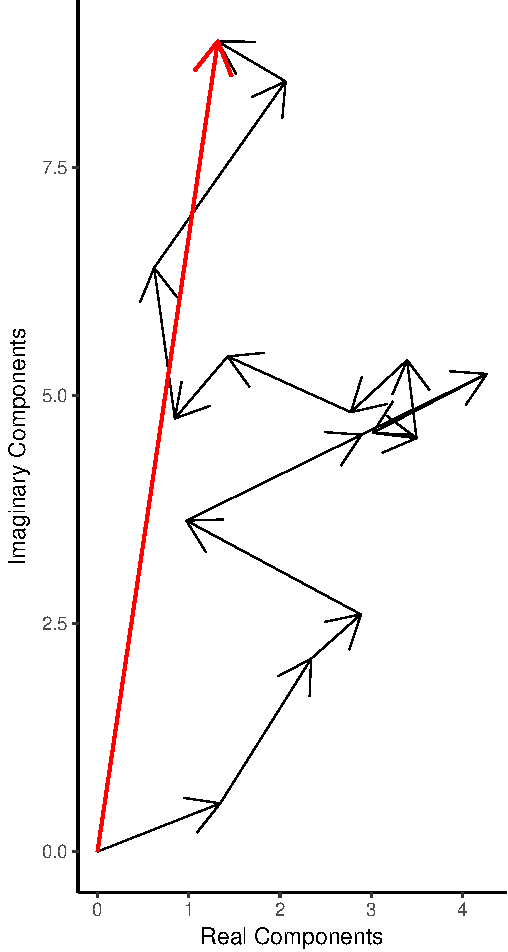
\includegraphics[width=\linewidth]{Scattering}
\caption{Example of complex scattering with $N=10$ elementary backscatterers}\label{Fig:ComplexScattering}
\end{marginfigure}

We have to make some assumptions in order to have a statistical description of the complex return $S$.
First, we are using microwaves whose typical wavelength is of the order of centimeters, and spatial resolutions of the order decimeters.
This leads to the first assumption: $N\to\infty$ if we are observing backscatterers whose size is smaller than the wavelength; think, for instance, of the case of imaging a grass field.
Second, there is no reason to expect that one or a few of these backscatterers dominate the return of the rest; there is no ``mirror'' in our resolution cell.
Third, the (non-negative) amplitudes $A_i$ are independent, with common mean.
Fourth, there is no reason to expect any particular organization or phase dominance; with this, we may assume that the phases $\phi_i$ are outcomes of independent identically distributed Uniform random variables with support $(-\pi,\pi]$.
Fifth, there is no association between phases and amplitudes.

With these hypothesis it is possible to prove that the real and imaginary parts of $S$ are independent Gaussian random variables with zero mean and the same variance $\sigma^2/2$; $\sigma^2$ is often referred to as backscatter.
Two targets with different backscatter only differ in the variance of their complex return $S$.

More often than not, instead of dealing directly with the complex scattering $S$ one prefers to handle its amplitude $A=|S|$ or intensity $I=|S|$.
Without loss of generality, we will prefer the latter.
If the real and imaginary parts of the complex scattering $S$ are independent zero-mean Gaussian random variables with variance $\sigma^2/2$, then the intensity follows an Exponential distribution with mean $\sigma^2$.

A unitary-mean exponential random variable has its distribution characterized by the density
\begin{equation}
f_Z(z) = e^{-z} \mathbb 1_{(0,\mathbb R_+)}(z),
\end{equation}
where $\mathbb 1_{A}(z)$ is the indicator function of the set $A$, i.e., it takes value $1$ inside $A$ and zero otherwise.
Denote this situation $Z\sim E(1)$, and notice that its expected value is $\E(Z)=1$ and its variance is $\Var(Z)=1$.

Being scale-invariant, if $Z'\sim E(1)$, then $Z=\sigma^2 Z'$ has density
\begin{equation}
f_Z(z) = \frac{1}{\sigma^2}e^{-z/\sigma^2} \mathbb 1_{(0,\mathbb R_+)}(z),
\end{equation}
and we denote this situation $Z\sim E(\sigma^2)$.
The cumulative distribution function of $Z\sim E(\sigma^2)$ is 
\begin{equation}
F_Z(z) = (1-e^{-z/\sigma^2}) \mathbb 1_{(0,\mathbb R_+)}(z).
\end{equation}

The mean and variance of $Z\sim E(\sigma^2)$ are, respectively, $\E(Z)=\sigma^2$ and $\Var(Z) = \sigma^4$.
With this, its coefficient of variation is one: $\CV(Z) = \sqrt{\Var(Z)}/\E(Z) = 1$.

Fig.~\ref{Fig:ExponentialDistribution} shows the densities, cumulative distribution functions and densities in semilogarithmic scale of three Exponential distributions, namely those with means equal to $1/2$, $1$ and $2$.

\begin{figure}[hbt]
\centering
\subfloat[Densities]{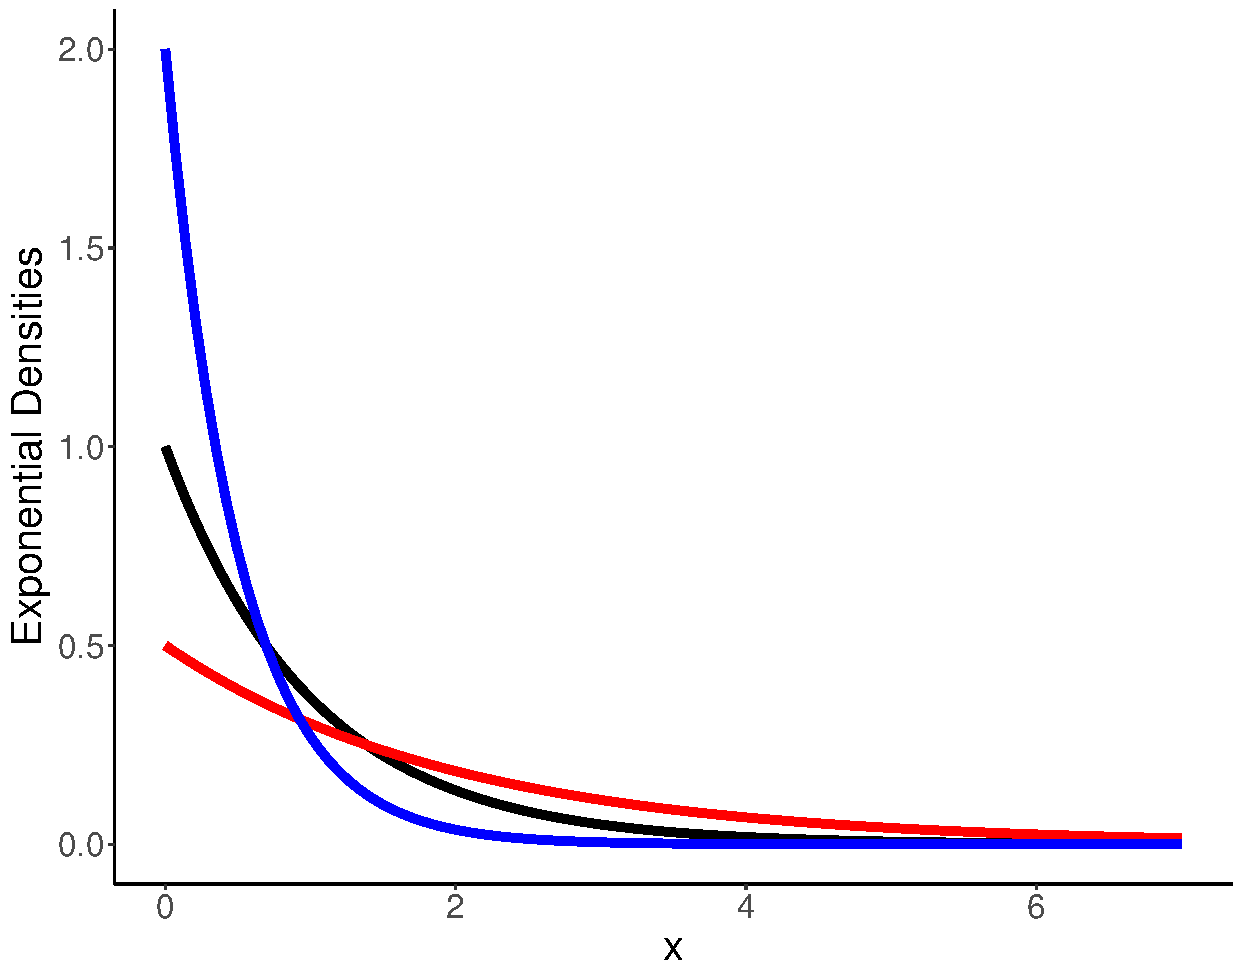
\includegraphics[width=.32\linewidth]{ExponentialDensities}}
\subfloat[Cumulative Distribution Functions]{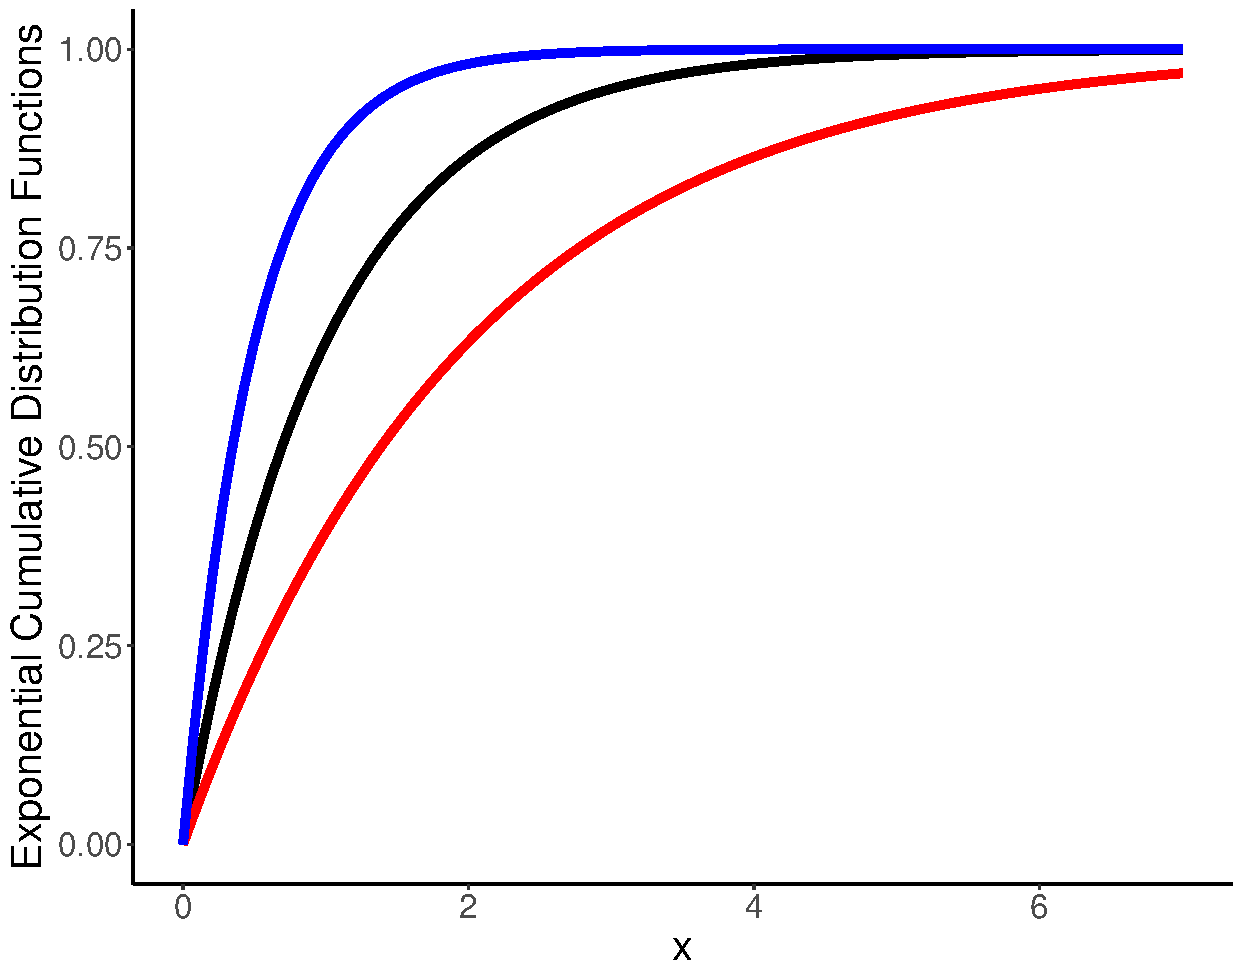
\includegraphics[width=.32\linewidth]{ExponentialCDFs}}
\subfloat[Densities in semilog scale]{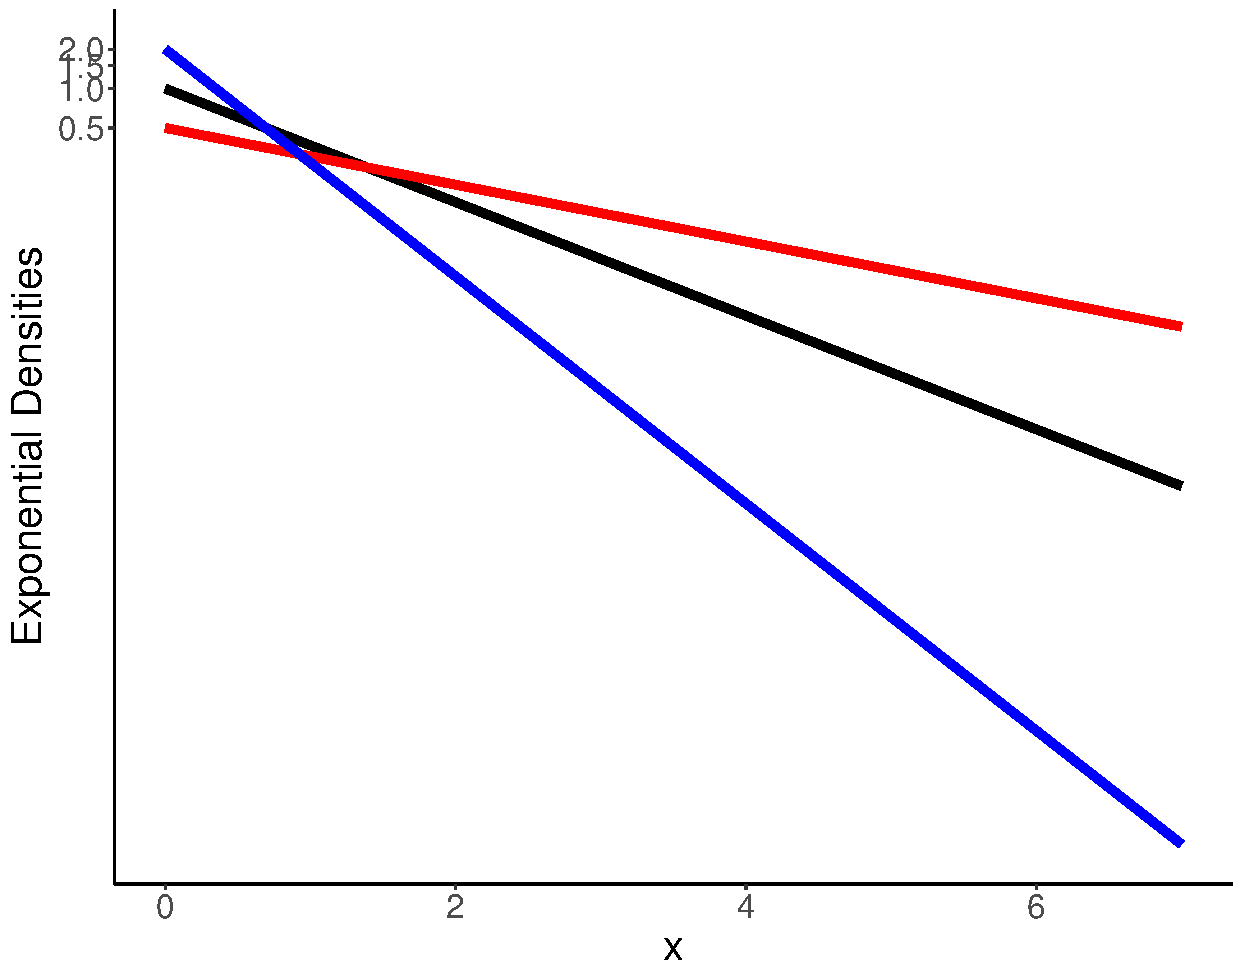
\includegraphics[width=.32\linewidth]{ExponentialDensitiesSemilog}}
\caption{Densities, cumulative distribution functions, and densities in semilogarithmic scale of the exponential distribution with means $1/2$, $1$ and $2$ (red, black, blue, resp.)}\label{Fig:ExponentialDistribution}
\end{figure}

The semilogarithmic scale is particularly useful at revealing the behavior of this distribution for large values: it is linear.

Multilook processing is often applied in order to improve the signal-to-noise ratio, which can be measured as the reciprocal of the coefficient of variation.
It consists of using the mean of $L$ independent observations:
\begin{equation}
Z = \frac1L \sum_{\ell=1}^{L} Z_\ell.
\end{equation}
If each $Z_\ell$ follows an exponential distribution with mean $\sigma^2$, we have that $Z$ obeys a Gamma distribution with mean $\sigma^2$ and shape parameter $L$.
This distribution is characterized by the density
\begin{equation}
f_Z(z;L,\sigma^2) = \frac{L^L}{\sigma^{2L}\Gamma(L)} z^{L-1} 
	\exp\big\{ -L z / \sigma^2
	\big\},
\end{equation}
where $\Gamma(\nu)$ is the Gamma function given by $\Gamma(\nu)=\int_{\mathbb R_+} t^{\nu-1} e^{-t} dt$.
The reader is referred to \citet{abramo-stegu64} for details and relationships with other important special functions.
We denote this situation $Z\sim\Gamma(\sigma^2,L)$
This is also a scale-invariant distribution, in the sense that if $Z'\sim\Gamma(1,L)$, then $Z=\sigma^2 Z'\sim \Gamma(\sigma^2,L)$.

Fig.~\ref{Fig:GammaDistribution} shows three cases of the Gamma distribution with unitary mean and shape parameters (Looks) equal to $1$ (the Exponential distribution), $3$ and $8$.

\begin{figure}[hbt]
\centering
\subfloat[Densities]{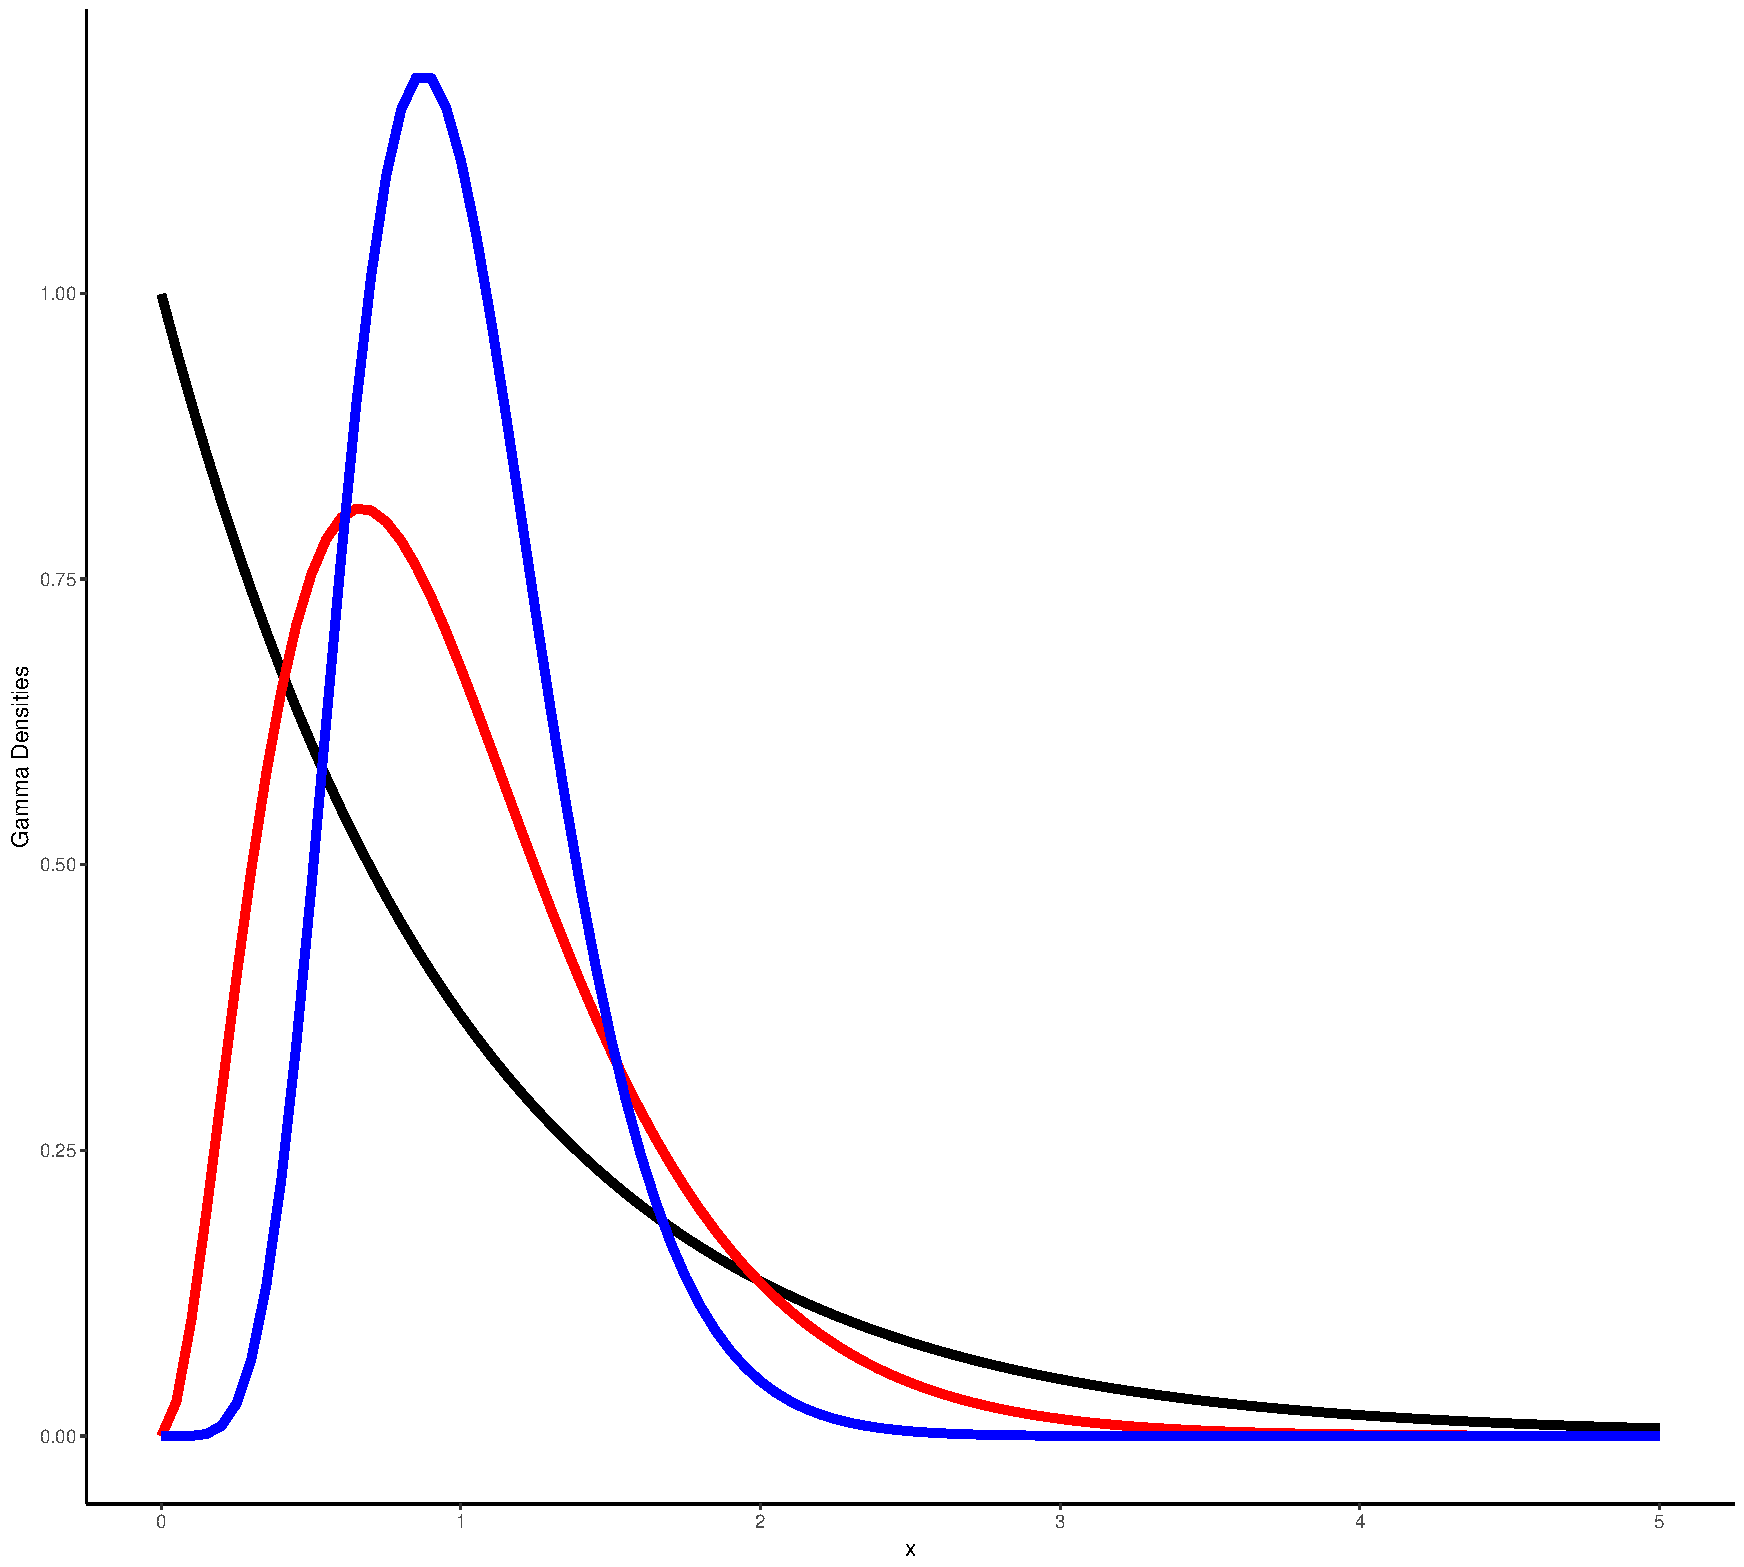
\includegraphics[width=.32\linewidth]{GammaDensities}}
\subfloat[Cumulative Distribution Functions]{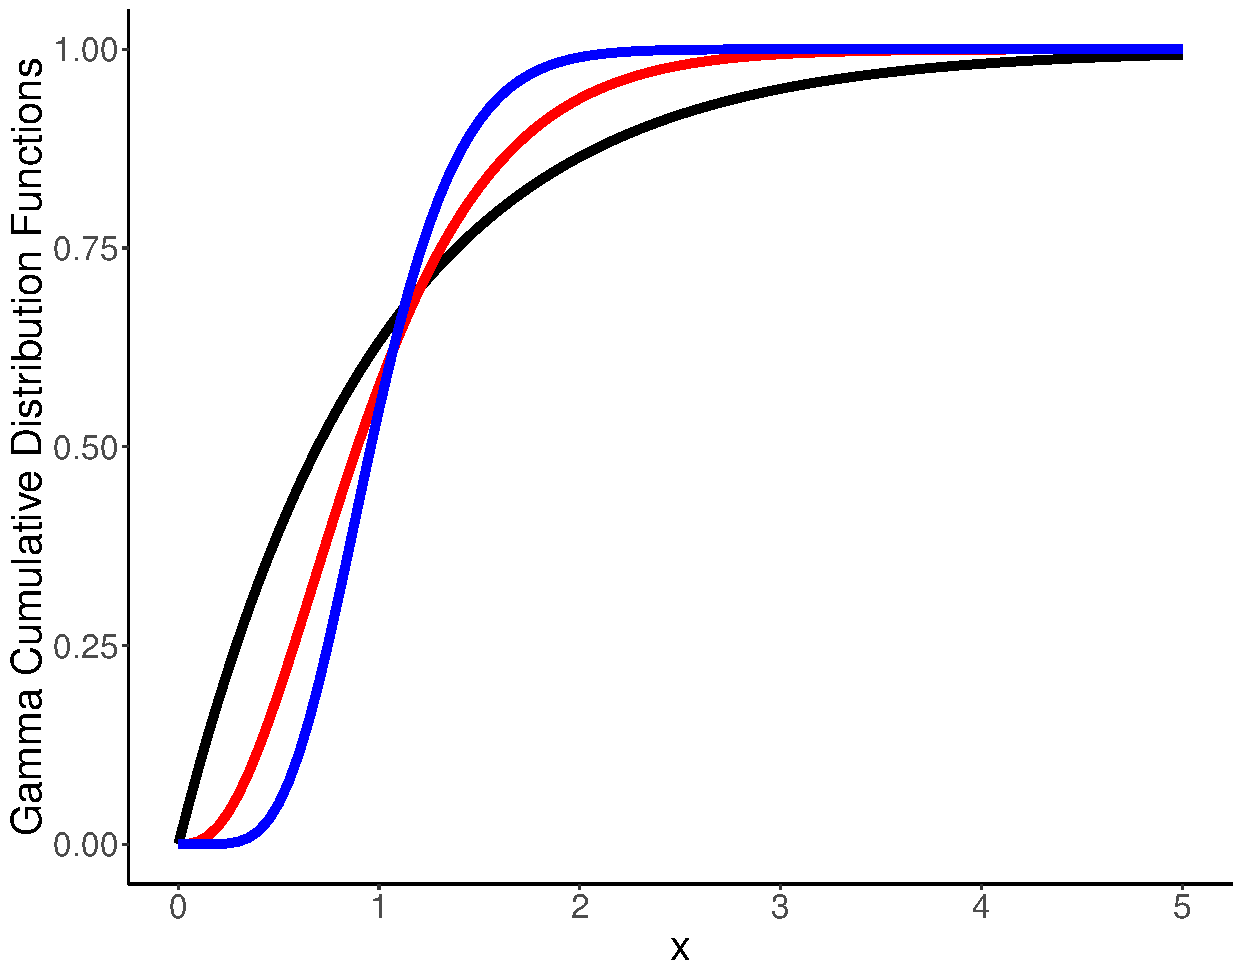
\includegraphics[width=.32\linewidth]{GammaCDFs}}
\subfloat[Densities in semilog scale\label{Fig:DensGammaSemilog}]{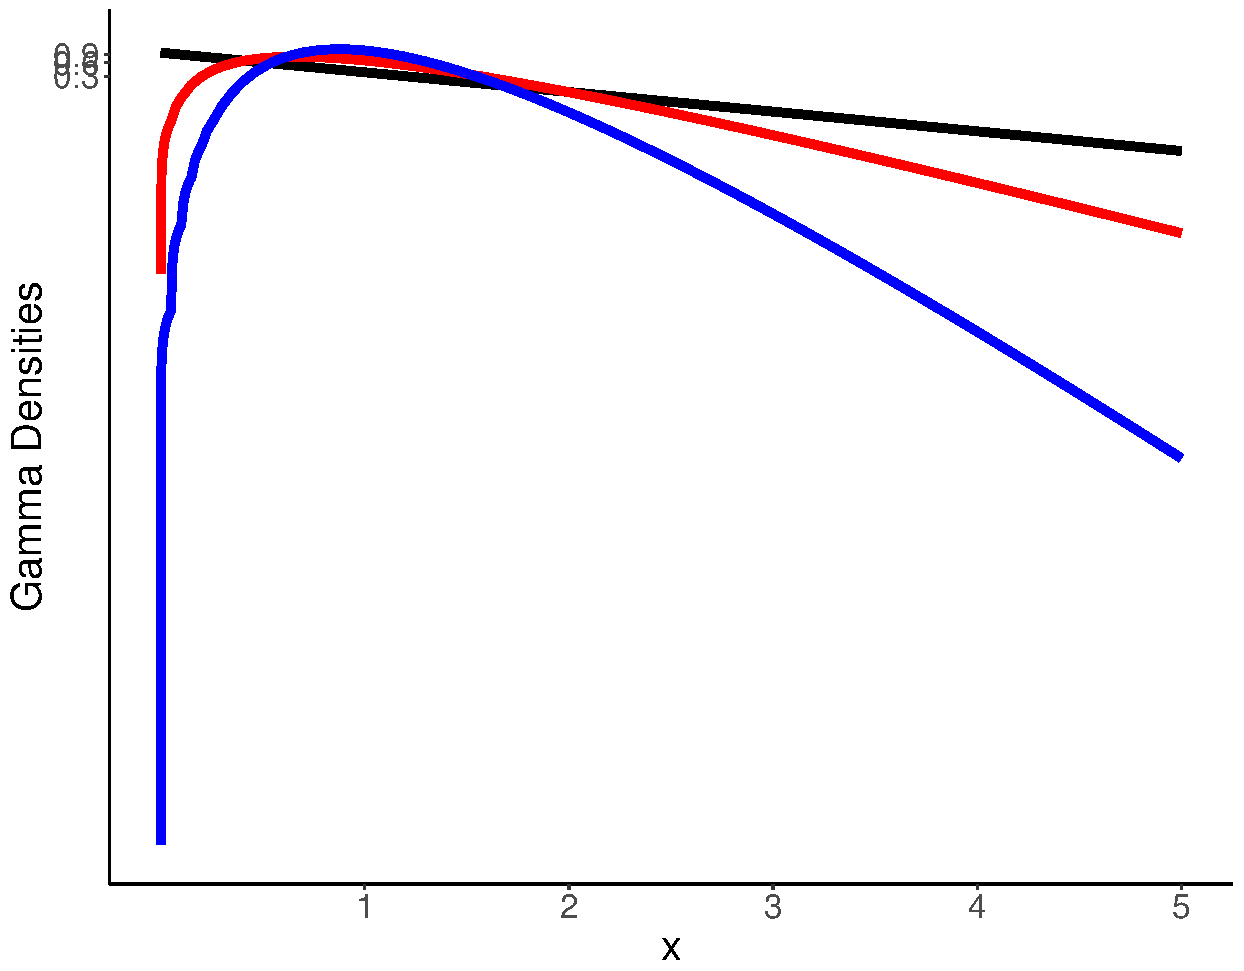
\includegraphics[width=.32\linewidth]{GammaDensitiesSemilog}}
\caption[Densities, cumulative distribution functions, and densities in semilogarithmic scale of the Gamma distribution with unitary mean and shape parameters $1$, $3$ and $8$]{Densities, cumulative distribution functions, and densities in semilogarithmic scale of the Gamma distribution with unitary mean and shape parameters $1$, $3$ and $8$ (red, black, blue, resp.)}\label{Fig:GammaDistribution}
\end{figure}

Fig.~\ref{Fig:GammaDistribution}\subref{Fig:DensGammaSemilog} is important, as this scale shows that the larger the number of looks, the less probable extreme events are.
The Exponential density, being linear

As we mentioned before, the intensity format is not the only possibility.
Assume $Z\sim\Gamma(\sigma^2,L)$ and that $g\colon\mathbb R_+ \to \mathbb R$ is a monotonic function with inverse $g^{-1}$.
The density of the random variable $W = g(Z)$ is given by 
\begin{equation}
f_W(w;L,\sigma^2) = \frac{L^L}{\sigma^{2L}\Gamma(L)} (g^{-1}(w)\big)' \big(g^{-1}(w)\big)^{L-1} 
	\exp\big\{ -L g^{-1}(w) / \sigma^2
	\big\},
	\label{eq:GammmaTransformed}
\end{equation}

Some authors\cite{IterativeWeightedMaximumLikelihoodDenoising} prefer the amplitude format $W=\sqrt{Z}$, while others\cite{Santos2017} opt for a logarithmic transformation $W=\log(Z+1)$ in order to obtain an additive (although not Gaussian) model for the data.
The model for the former is known as \textit{Square Root of Gamma} or \textit{Nakagami} distribution,
while the one for the latter is know as the \textit{Fisher-Tippet} distribution when $L=1$.
The reader is invited to obtain these densities using~\eqref{eq:GammmaTransformed}.

\begin{exer}
Find the densities of the Nakagami and Fisher-Tippet distributions.
Illustrate them.
\end{exer}

\begin{exer}
Assume $Z$ follows a Nakagami distribution.
Find the density of $W=\log(Z+1)$ (a multilook Fisher-Tippet distribution).
Illustrate.
\end{exer}

\chapter{The Multiplicative Model}\label{Chapter:MultiplicativeModel}

\newthought{One of the most famous statistical aphorisms} is due to Prof.\ George Box\cite{StatisticsForExperimenters}:
\begin{quotation}
The most that can be expected from any model is that it can supply a useful approximation to reality:

\textbf{All models are wrong; some models are useful.}
\end{quotation}
In line with this idea, in this chapter we will discuss the most important and illuminating models for SAR data that generalize the one for textureless data.

The Multiplicative Model is just one of the infinitely many ways to build stochastic descriptions for SAR data.
Among its advantages we would like to mention that it can be considered an \textit{ab initio} model, and that it leads to expressive and tractable descriptions of the data.

Let us recall that the basic model for multilook intensity data is the $\Gamma(\sigma^2,L)$ law whose density is
\begin{equation}
f_Z(z;L,\sigma^2) = \frac{L^L}{\sigma^{2L}\Gamma(L)} z^{L-1} 
	\exp\big\{ -L z / \sigma^2
	\big\}.
\end{equation}
As previously said, the Gamma distribution is scale-invariant, so we may pose this model as the product between the constant backscatter $X=\sigma^2$ and the multilook speckle $Y\sim\Gamma(1,L)$.

But, are there situations were we cannot assume a constant backscatter?
Yes, there are.

A constant backscatter results from infinitely many elementary backscatterers, i.e.\ from the assumption that $N\to\infty$ in~\eqref{Eq:ComplexBackscatter} (page~\pageref{Eq:ComplexBackscatter}).
Such assumption makes the particular choice of the sensed area irrelevant.
But this may not be the case always.

The advent of higher resolution sensors makes this hypothesis unsuitable in areas where the elementary backscatterers are of the order of the wavelength; cf.\ Table~\ref{Tab:Bands}.
If, for instance, we are dealing with a \SI{1x1}{\meter} resolution image, we may consider $N\to\infty$ if the target is flat and composed of grass;
but if the target is a forest, this assumption may be unrealistic.

\section{The $\mathcal K$ distribution}

\citet{JakemanPusey76} were among the first who tackled this problem.
Assuming that the number of elementary backscatterers $N$ fluctuates according to a Negative Binomial distribution (see Section~\ref{Sec:NegativeBinomial}), they obtained a closed-form density which characterizes the $\mathcal K$ distribution:
\begin{equation}
f_Z(z;\alpha,\lambda,L) =
\frac{2\lambda L}{\Gamma(\alpha)\Gamma(L)} (\lambda L z)^{\frac{\alpha+L}{2}-1} K_{\alpha-L}(2\sqrt{\lambda L z}),
\label{Eq:DensKI}
\end{equation}
where $\alpha>0$ measures the roughness, $\lambda>0$ is a scale parameter, and $K_\nu$ is the modified Bessel function of order $\nu$.
This special function is given by $K_\nu (z) = \int_0^\infty e^{-z} \cosh (\nu t) dt$.
See the book by \citet{Gradshteyn80} for other definitions and important properties.
This function is implemented in many numerical platforms as, for instance, in \texttt R.

We denote $Z\sim \mathcal K(\alpha,\lambda,L)$ the situation of $Z$ following the distribution characterized by~\eqref{Eq:DensKI}.
The $k$-order moments of $Z$ are
\begin{equation}
E(Z^k) = (\lambda L)^{-k} \frac{\Gamma(L+k)\Gamma(\alpha+k)}{\Gamma(L)\Gamma(\alpha)}.
\label{Eq:MomentKI}
\end{equation}
Eq.~\eqref{Eq:MomentKI} is useful, among other applications, for finding $\lambda^*=\alpha$, the scale parameter that yields a unitary mean distribution for each $\alpha$ and any $L$.

Fig.~\ref{Fig:KIDistribution} shows the densities in linear and semilogarithmic scales of the Exponential and $\mathcal K$ distributions.
They all have unitary mean, and the latter is shown with different degrees of roughness ($\alpha\in\{1,3,8\}$).
It is noticeable that the larger the value of $\alpha$ is, the closer the $\mathcal K$ and $\text{E}$ densities become.
In fact, \citet{frery96} prove that there is convergence in distribution of the latter to the former.

\begin{figure}[hbt]
\centering
\subfloat[Densities]{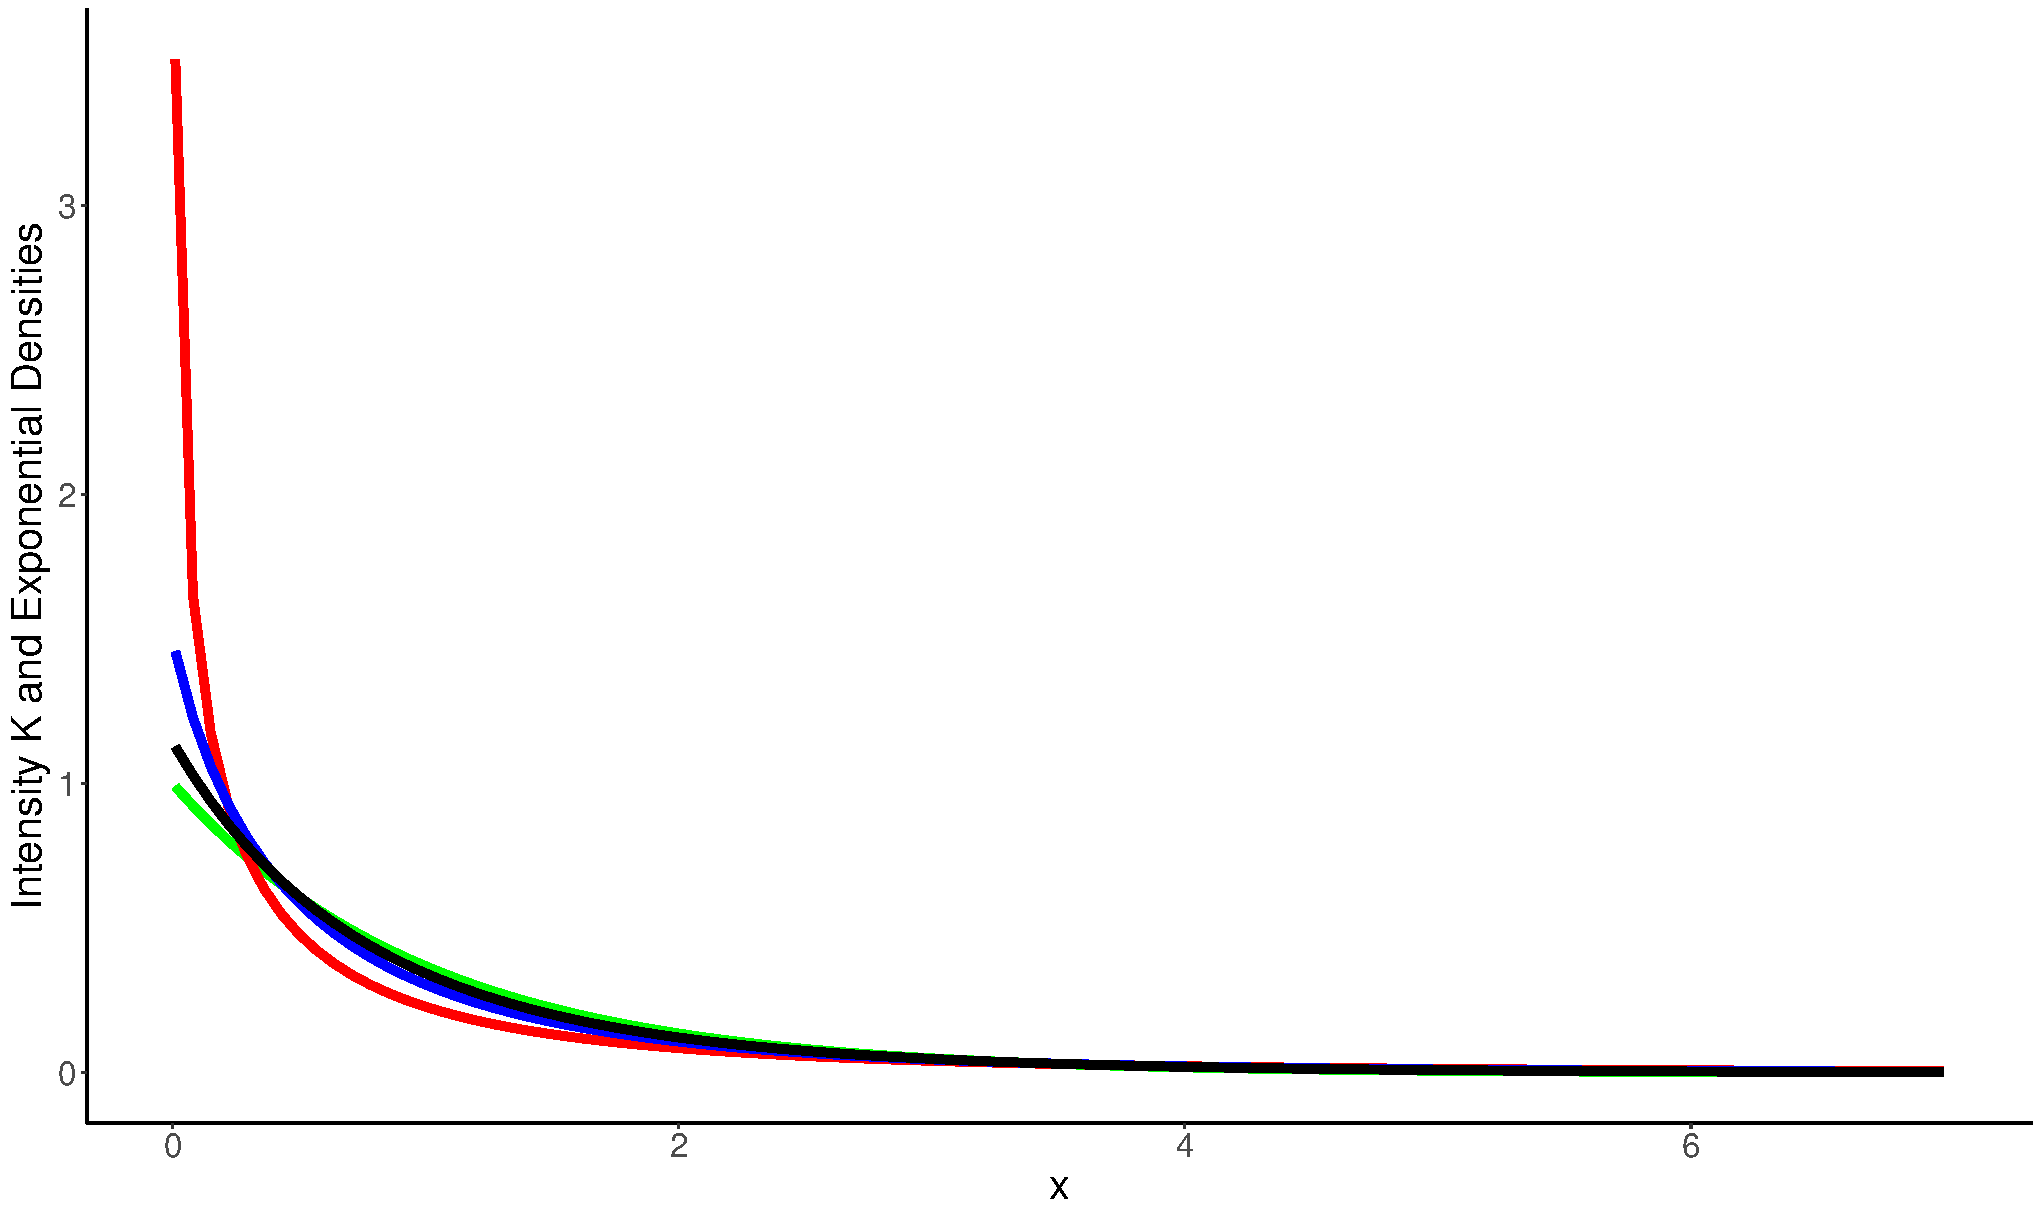
\includegraphics[width=.48\linewidth]{KIDensities}}
\subfloat[Densities in semilog scale\label{Fig:DensKISemilog}]{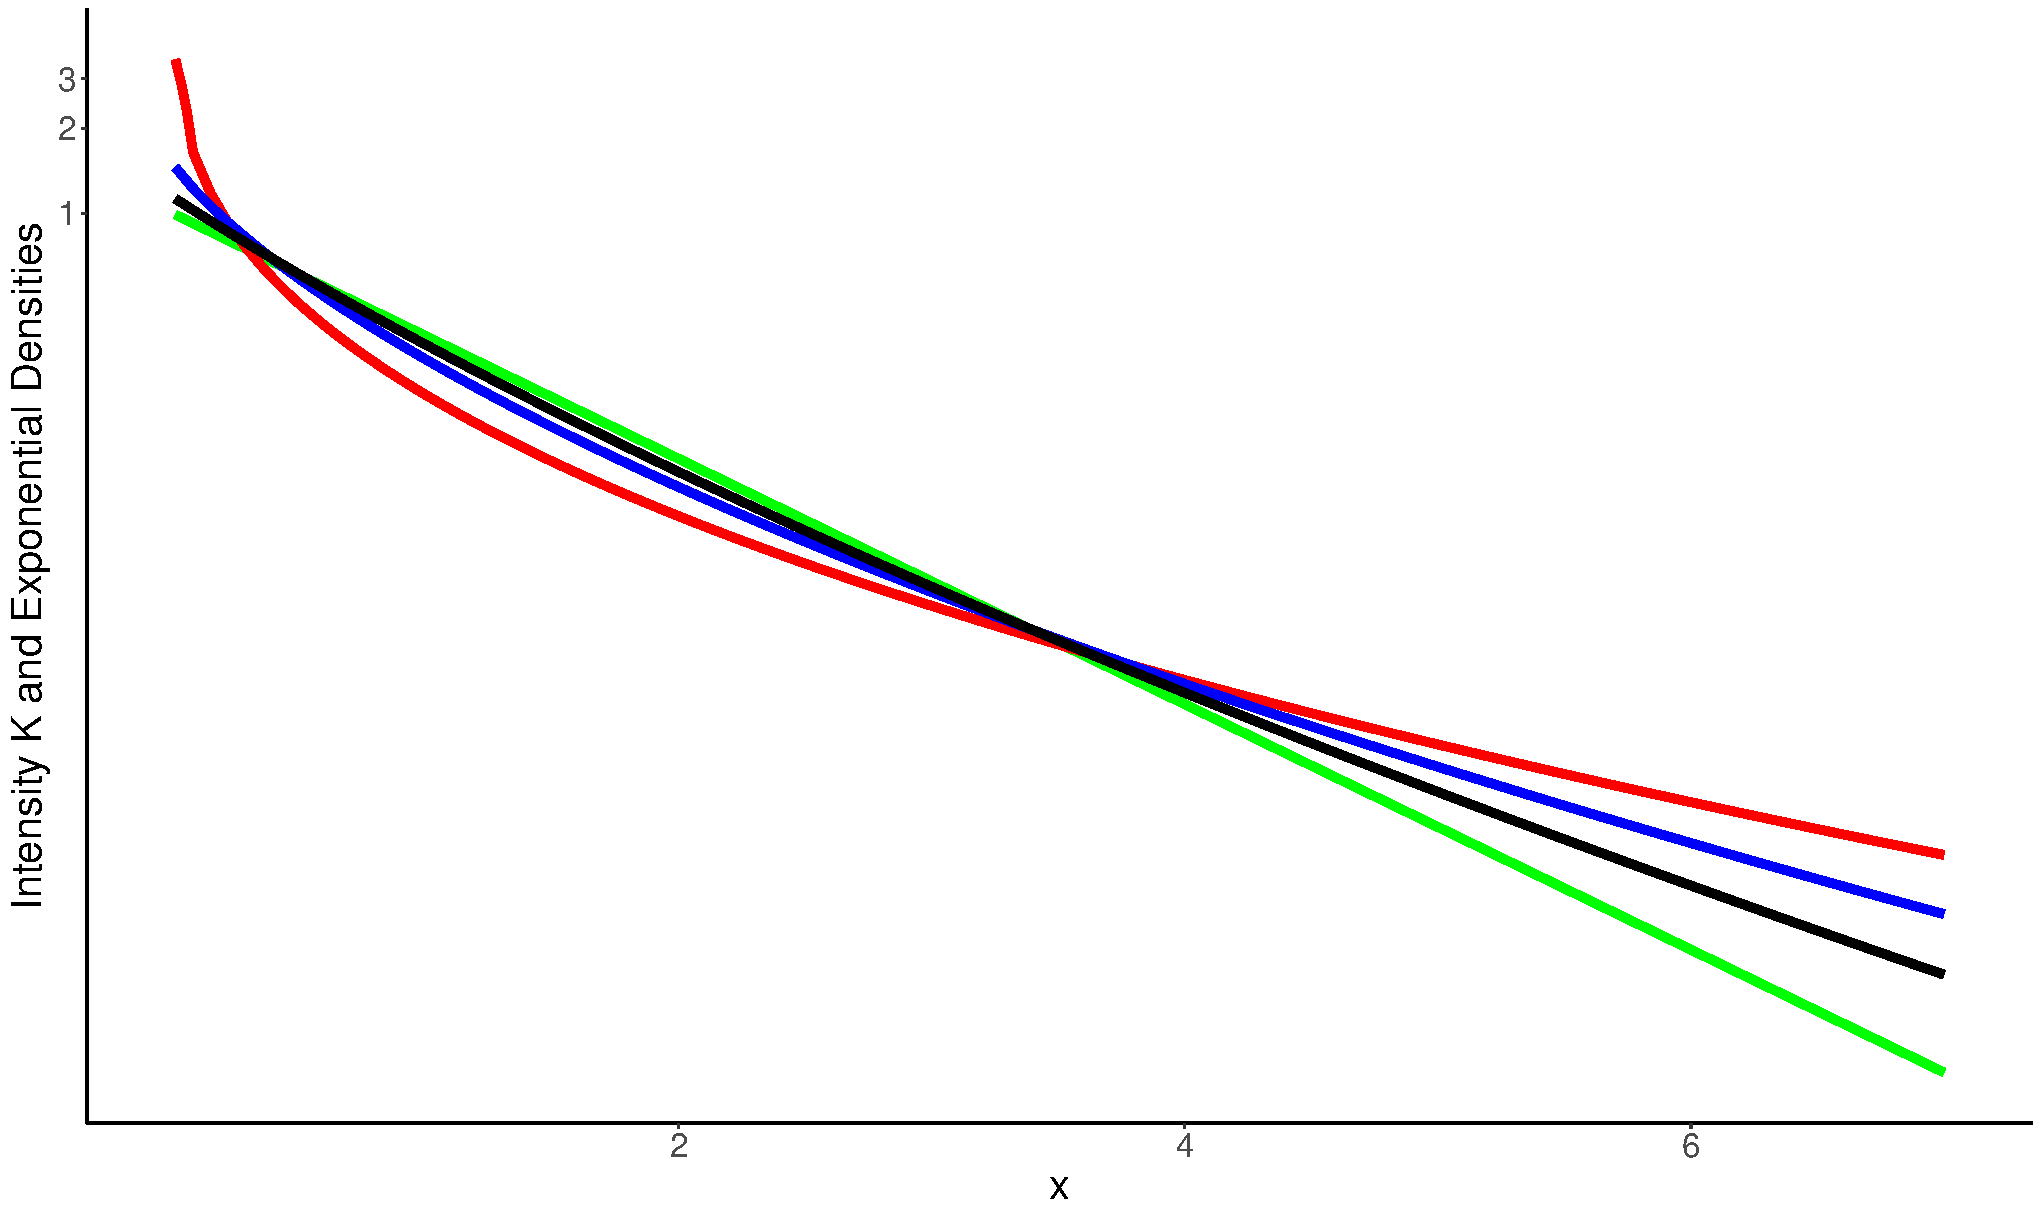
\includegraphics[width=.48\linewidth]{KIDensitiesSemilog}}
\caption[Densities in linear and semilogarithmic scale of the $\text{E}(1)$ (green) and $\mathcal K$ distributions]{Densities in linear and semilogarithmic scale of the $\text{E}(1)$ (green) and $\mathcal K$ distributions with unitary mean ($\alpha\in\{1,3,8\}$ in red, blue, and black, resp.)}\label{Fig:KIDistribution}
\end{figure}

The difference between these distributions is noteworthy, c.f.\ Fig.~\ref{Fig:KIDistribution}\subref{Fig:DensKISemilog}.
The green straight line is the density of the Exponential distribution, while the red one is that of the $\mathcal K(1,1,1)$ law.
The latter assigns larger probabilities to both small and large values, when compared with the former.
This leads, as will be seen later, to very contrasted data.

Fig.~\ref{Fig:KIDistributionLooks} shows the effect of varying the number of looks, for the same $\alpha=2$ and $\lambda=2$.

\begin{figure}[hbt]
\centering
\subfloat[Densities]{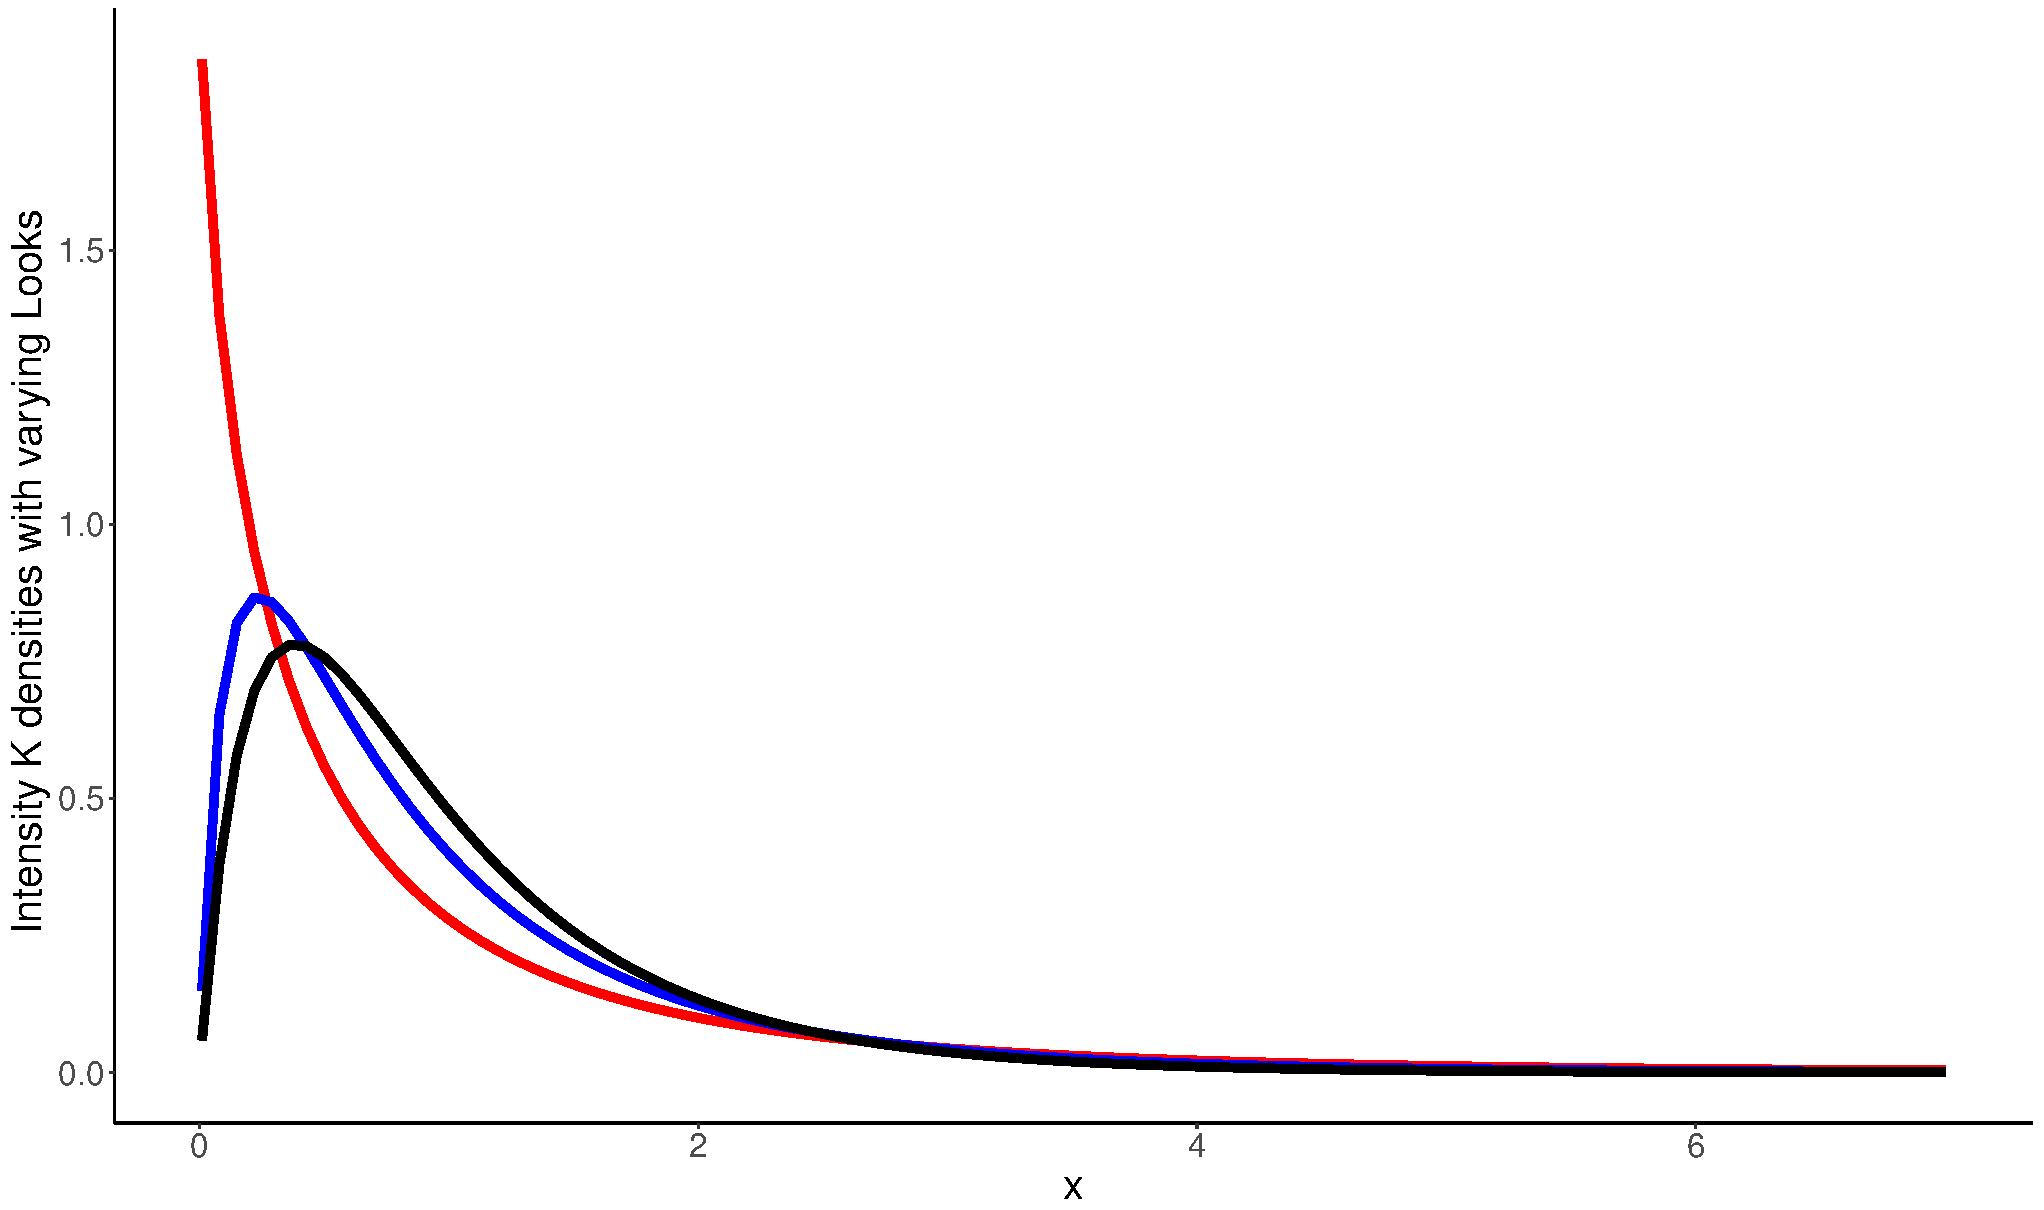
\includegraphics[width=.48\linewidth]{KIDensitiesLooks}}
\subfloat[Densities in semilog scale\label{KIDensitiesSemilog}]{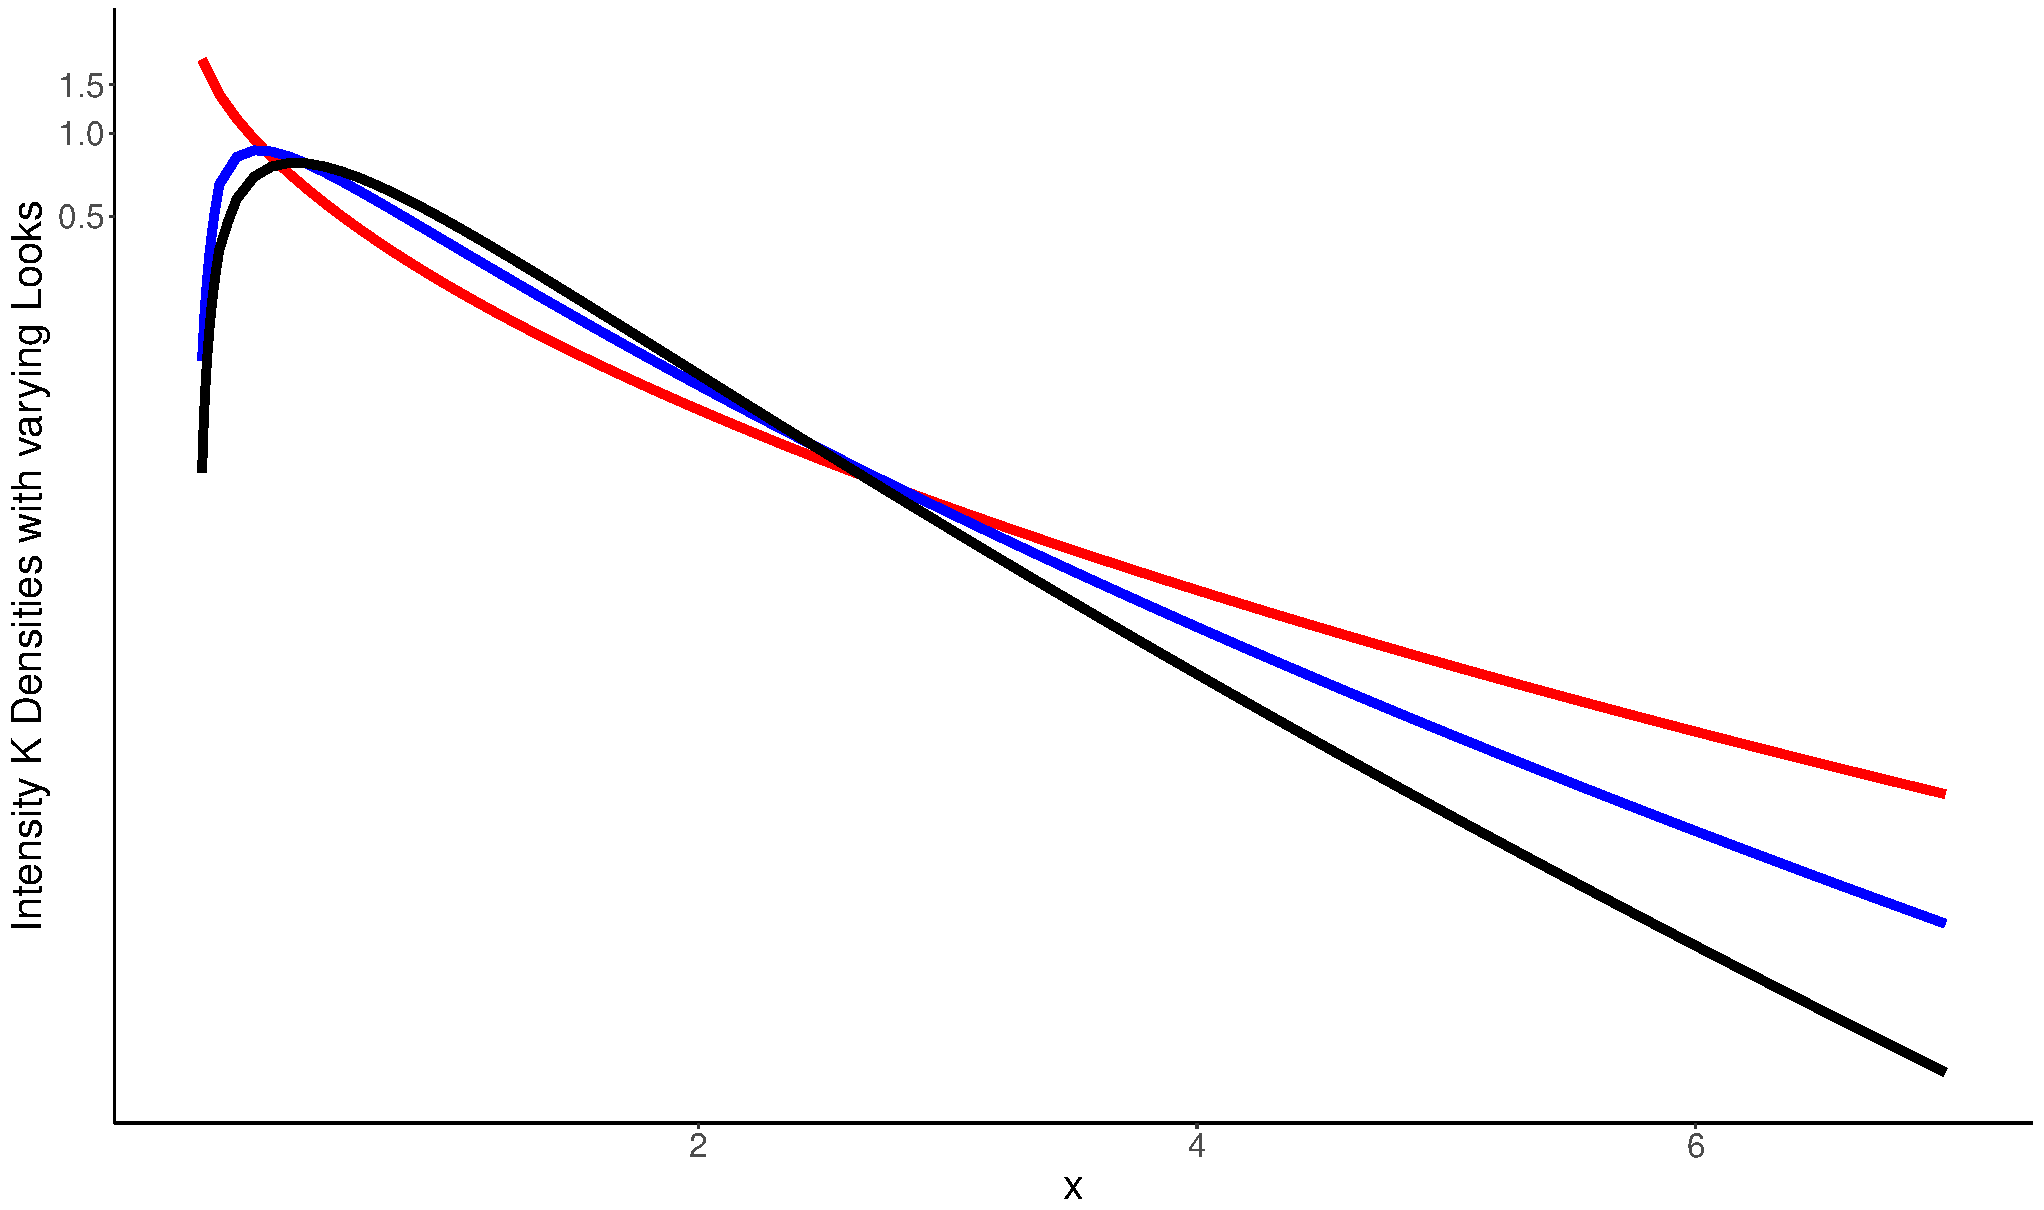
\includegraphics[width=.48\linewidth]{KIDensitiesSemilogLooks}}
\caption[Densities in linear and semilogarithmic scale $\mathcal K(2,2,L)$ distributions with unitary mean and $L\in\{1,3,8\}$]{Densities in linear and semilogarithmic scale $\mathcal K(2,2,L)$ distributions with unitary mean and $L\in\{1,3,8\}$ in red, blue, and black, resp.)}\label{Fig:KIDistributionLooks}
\end{figure}

Notice in Fig~\ref{Fig:KIDistributionLooks}\subref{KIDensitiesSemilog} the dramatic effect multilook processing has mostly on the distribution of very small values.
This, along with the reduced probability very large values have with multilook processing, yields less contrasted images.

Although the basic construction, and physical explanation, of the $\mathcal K$ distribution stems from letting fluctuate the number of elementary backscatterers, we are interested in an equivalent derivation.

As previously said, the basic model for observations without roughness is~\eqref{eq:SARGammaDensity}.
The mean $X=\sigma^2$ can be seen as multiplying $Y$, a $\Gamma(1,L)$ random variable, which describes the speckle.
As we are interested in letting the mean fluctuate, $X$ can be described by any distribution with positive support.
If we choose a Gamma random variable with mean $\alpha/\lambda>0$ and shape parameter $\alpha>0$, i.e., $Y\sim\Gamma(\alpha/\lambda,\alpha)$, and further assume that $X$ and $Y$ are independent, then the product $Z=XY$ follows a $\mathcal{K}(\alpha,\lambda,L)$ distribution with density~\eqref{Eq:DensKI}.
This \textit{multiplicative} construction is not only useful for sampling from this distribution, but also for obtaining other models for the return.

\section{The $\mathcal G^0$ distribution}

In this line, \citet{frery96} noticed that the $\mathcal{K}$ distribution failed at describing data from extremely textured areas as, for instance, urban targets.
The authors then proposed a different model for the backscatter $X$: the Reciprocal Gamma distribution.

We say that $X\sim{\Gamma^{-1}}(\alpha,\gamma)$, with $\alpha<0$ and $\gamma>0$ follows a 
Reciprocal Gamma distribution is characterized by the density
\begin{equation}
f_X(x;\alpha,\gamma) = \frac{1}{\gamma^\alpha} x^{\alpha-1} \exp\{-\gamma/x\},
\label{Eq:IGdensity}
\end{equation}
for $x>0$ and zero otherwise.

Now introducing the Reciprocal Gamma model for the backscatter in the multiplicative model, i.e. by multiplying the independent random variables $X\sim{\Gamma^{-1}}(\alpha,\gamma)$ and $Y\sim\Gamma(1,L)$, one obtains the $\mathcal{G}^0$ distribution for the return $Z=XY$, which is characterized by the density
\begin{equation}
f_Z(z; \alpha,\gamma,L) = \frac{L^L \Gamma(L-\alpha)}{\gamma^\alpha \Gamma(L)\Gamma(-\alpha)} \frac{z^{L-1}}{(\gamma+L z)^{L-\alpha}},
\label{Eq:DensGI0}
\end{equation}
where $\alpha<0$, and $\gamma,z>0$.
It is noteworthy that, differently from~\eqref{Eq:DensKI}, this density does not involve Bessel functions.

We denote $Z\sim \mathcal G^0(\alpha,\gamma,L)$ the situation of $Z$ following the distribution characterized by~\eqref{Eq:DensGI0}.
The $k$-order moments of $Z$ are
\begin{equation}
E(Z^k) = (\gamma / L)^{k} \frac{\Gamma(L+k)\Gamma(-\alpha-k)}{\Gamma(L)\Gamma(-\alpha)},
\label{Eq:MomentGI0}
\end{equation}
provided $-\alpha>k$, and infinite otherwise.
Eq.~\eqref{Eq:MomentGI0} is useful, among other applications, for finding $\gamma^*=-\alpha-1$, the scale parameter that yields a unitary mean distribution for each $\alpha$ and any $L$.

Fig.~\ref{Fig:GI0Distribution} shows the $\text{E}(1)$ and $\mathcal G^0(\alpha,\gamma^*, 1)$ densities.
The differences in tail behavior are clearly exhibited in the semilogarithmic scale; cf.\ Fig.~\ref{Fig:GI0Distribution}\subref{Fig:DensGI0Semilog}.
Whereas the exponential distribution decreases linearly, the $\mathcal G^0$ law assigns more probability to larger events increasing, thus, the variability of the return.

\begin{figure}[hbt]
\centering
\subfloat[Densities]{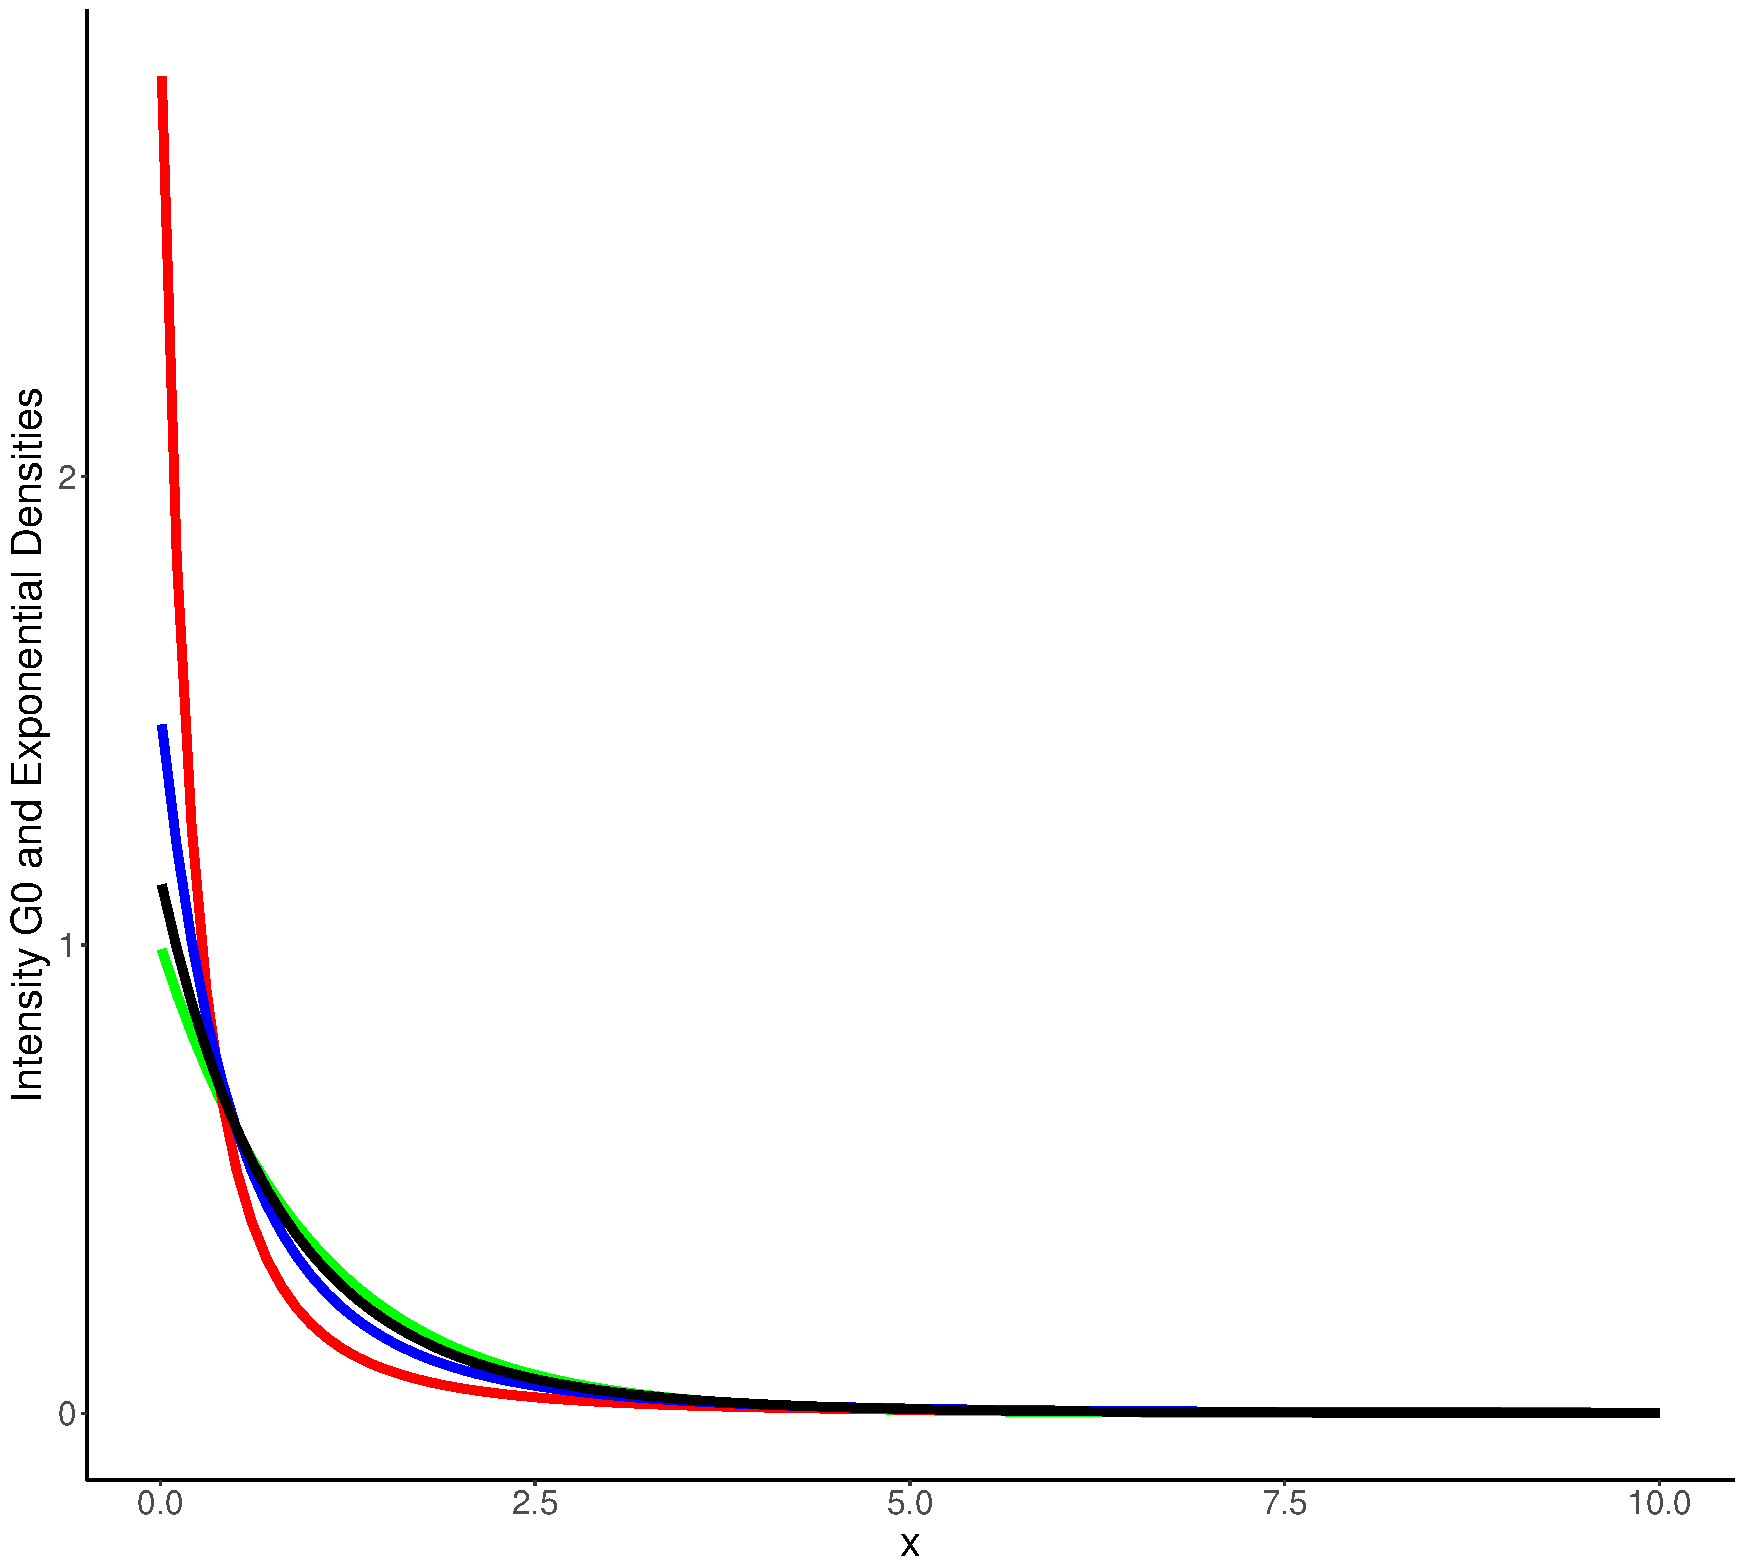
\includegraphics[width=.48\linewidth]{GI0Densities}}
\subfloat[Densities in semilog scale\label{Fig:DensGI0Semilog}]{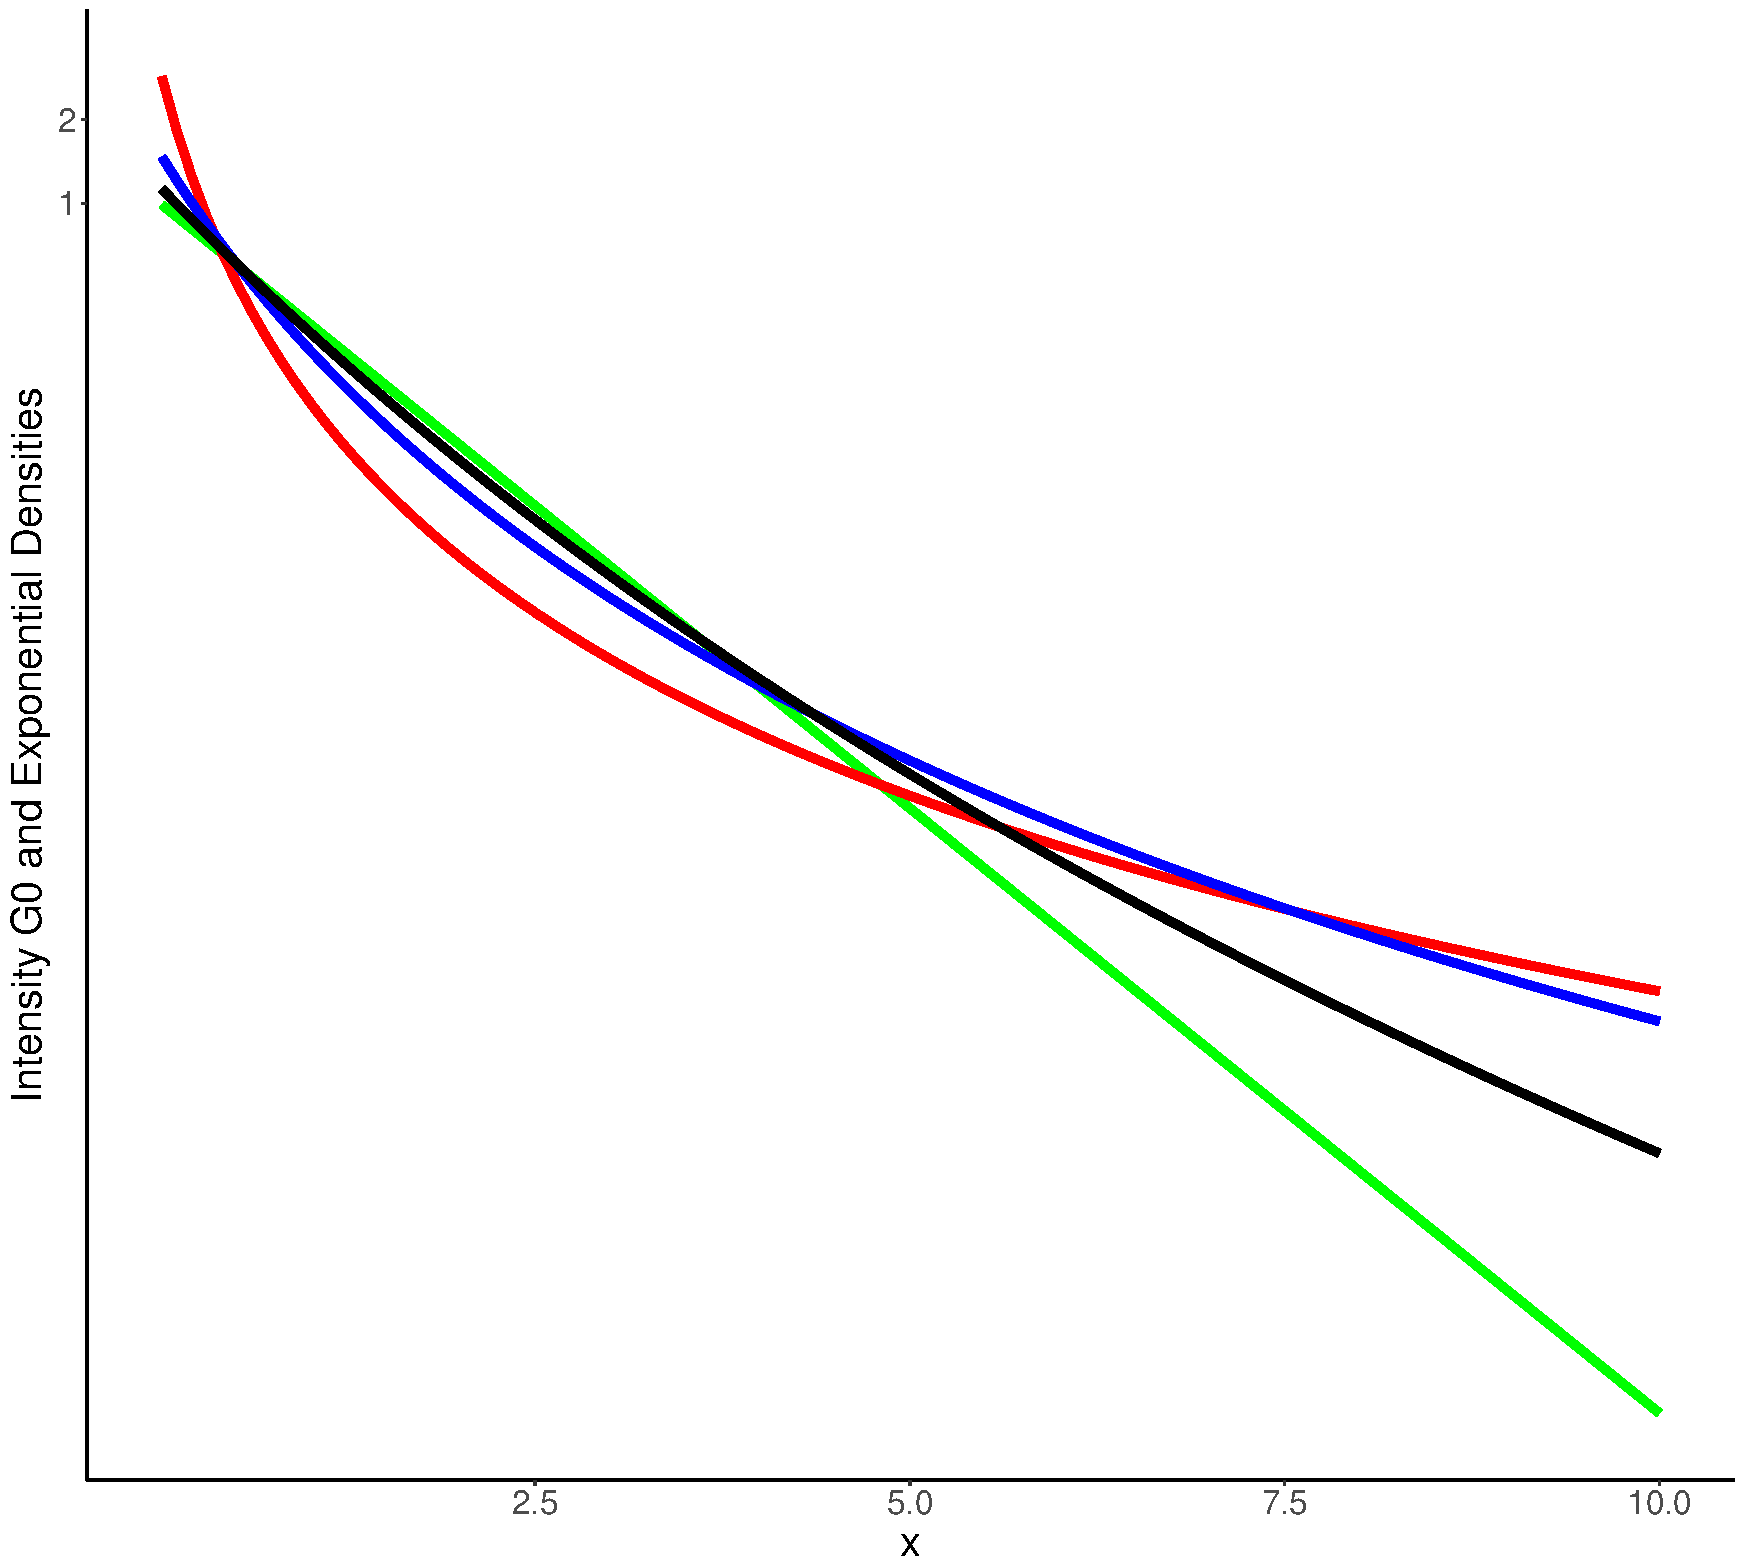
\includegraphics[width=.48\linewidth]{GI0DensitiesSemilog}}
\caption[Densities in linear and semi-logarithmic scale of the $\text{E}(1)$ (green) and $\mathcal G^0$ distributions with unitary mean]{Densities in linear and semi-logarithmic scale of the $\text{E}(1)$ (green) and $\mathcal G^0$ distributions with unitary mean and $\alpha\in\{-1.5,-3,-8\}$ in red, blue, and black, resp.}\label{Fig:GI0Distribution}
\end{figure}

Fig.~\ref{Fig:GI0DistributionLooks} shows the effect of varying the number of looks, for the same $\alpha=5$ and $\gamma=4$.

Notice, again, in Fig~\ref{Fig:GI0DistributionLooks}\subref{GI0DensitiesSemilog} the effect multilook processing has mostly on the distribution of very small values.
This, along with the reduced probability very large values have with multilook processing, yields less contrasted images.

\begin{figure}[hbt]
\centering
\subfloat[Densities]{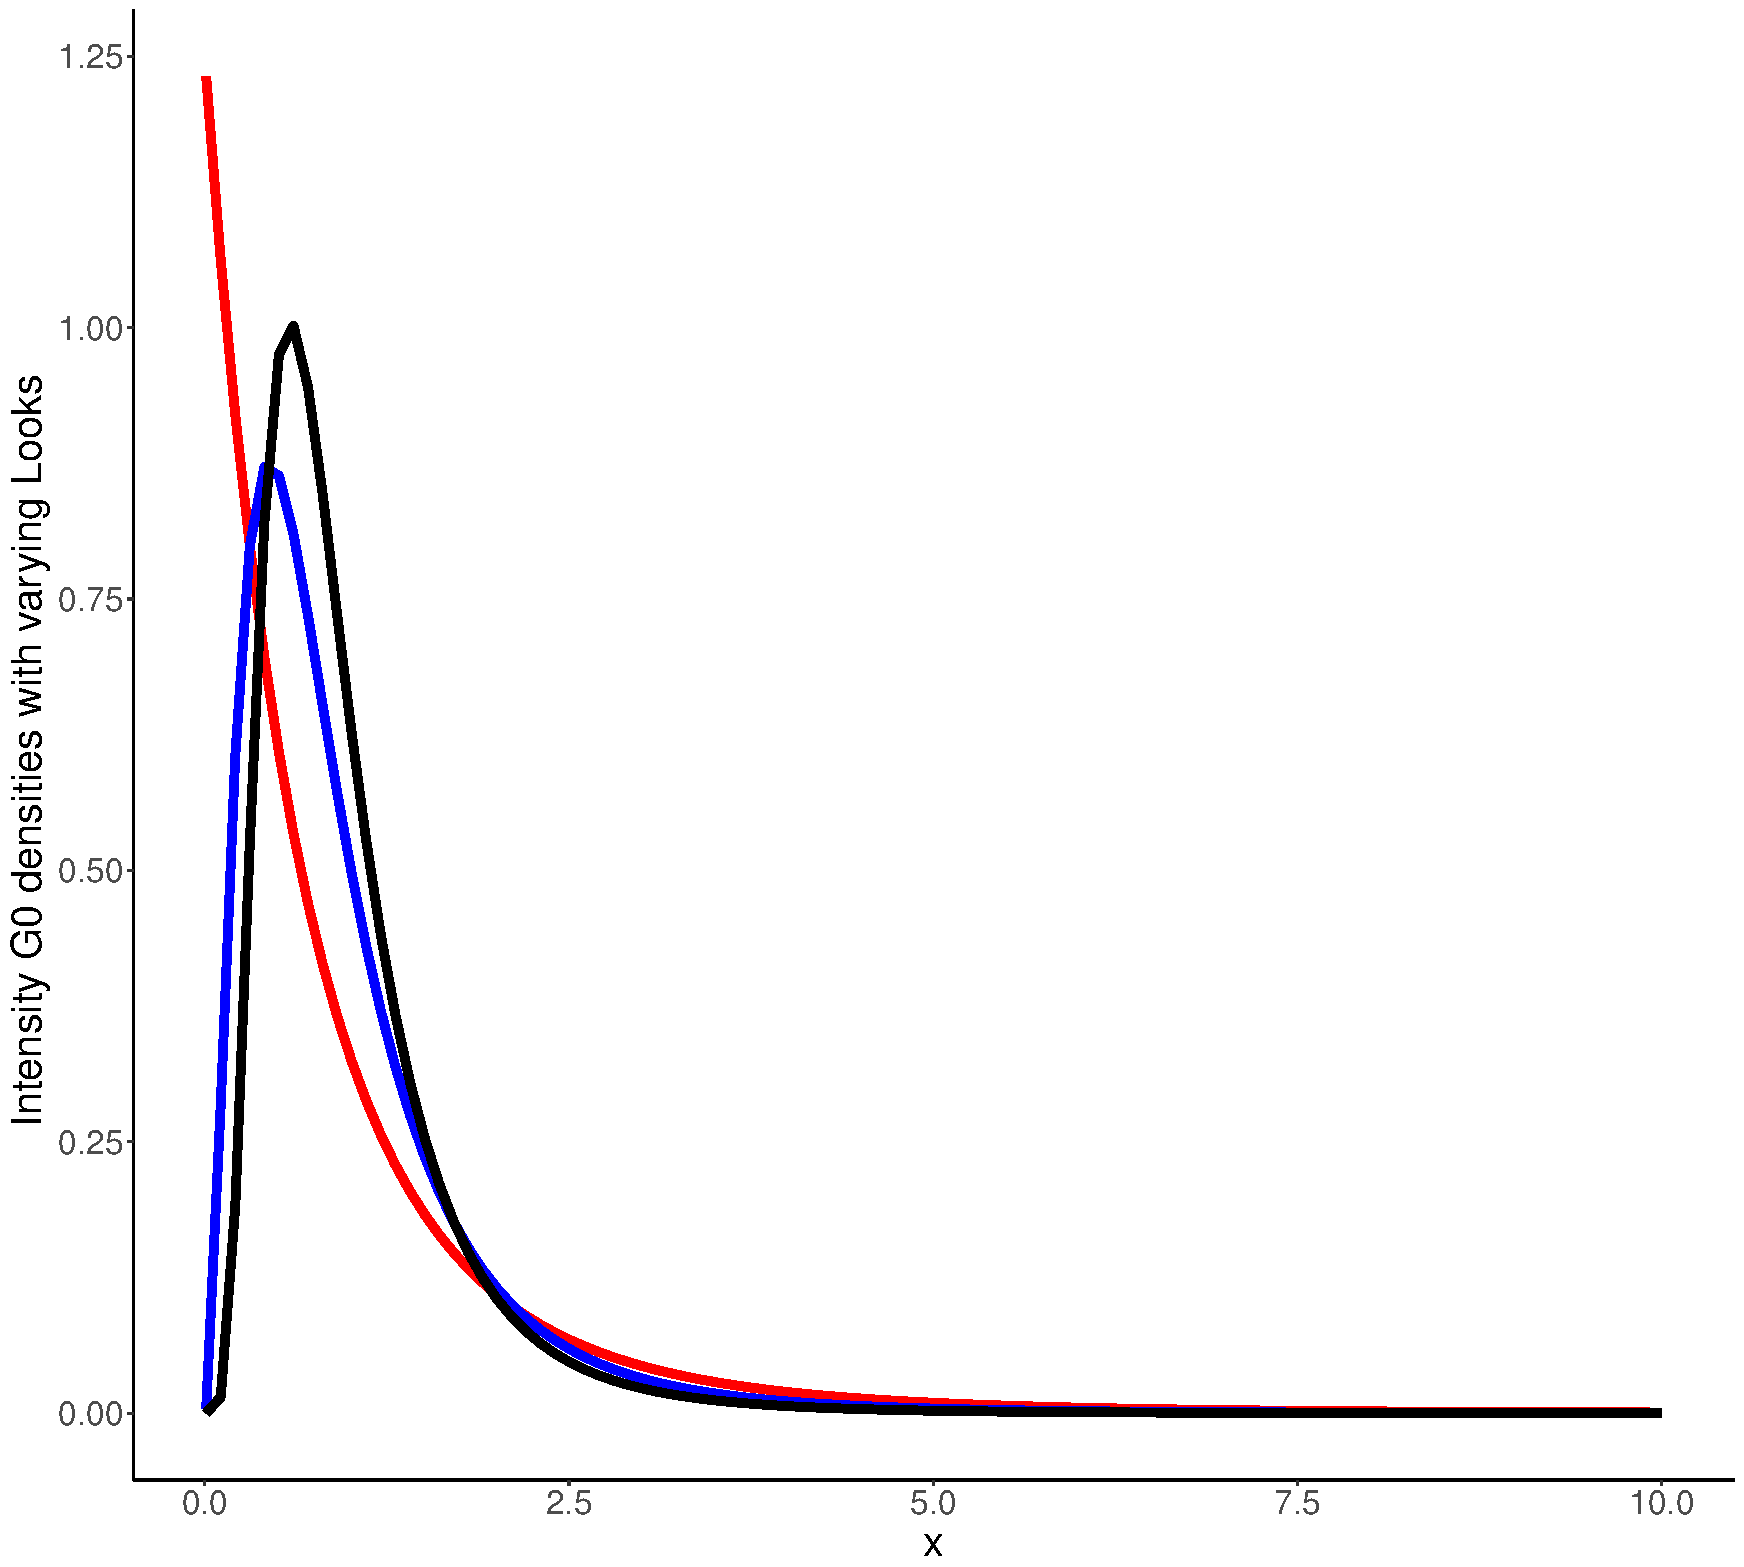
\includegraphics[width=.48\linewidth]{GI0DensitiesLooks}}
\subfloat[Densities in semilog scale\label{GI0DensitiesSemilog}]{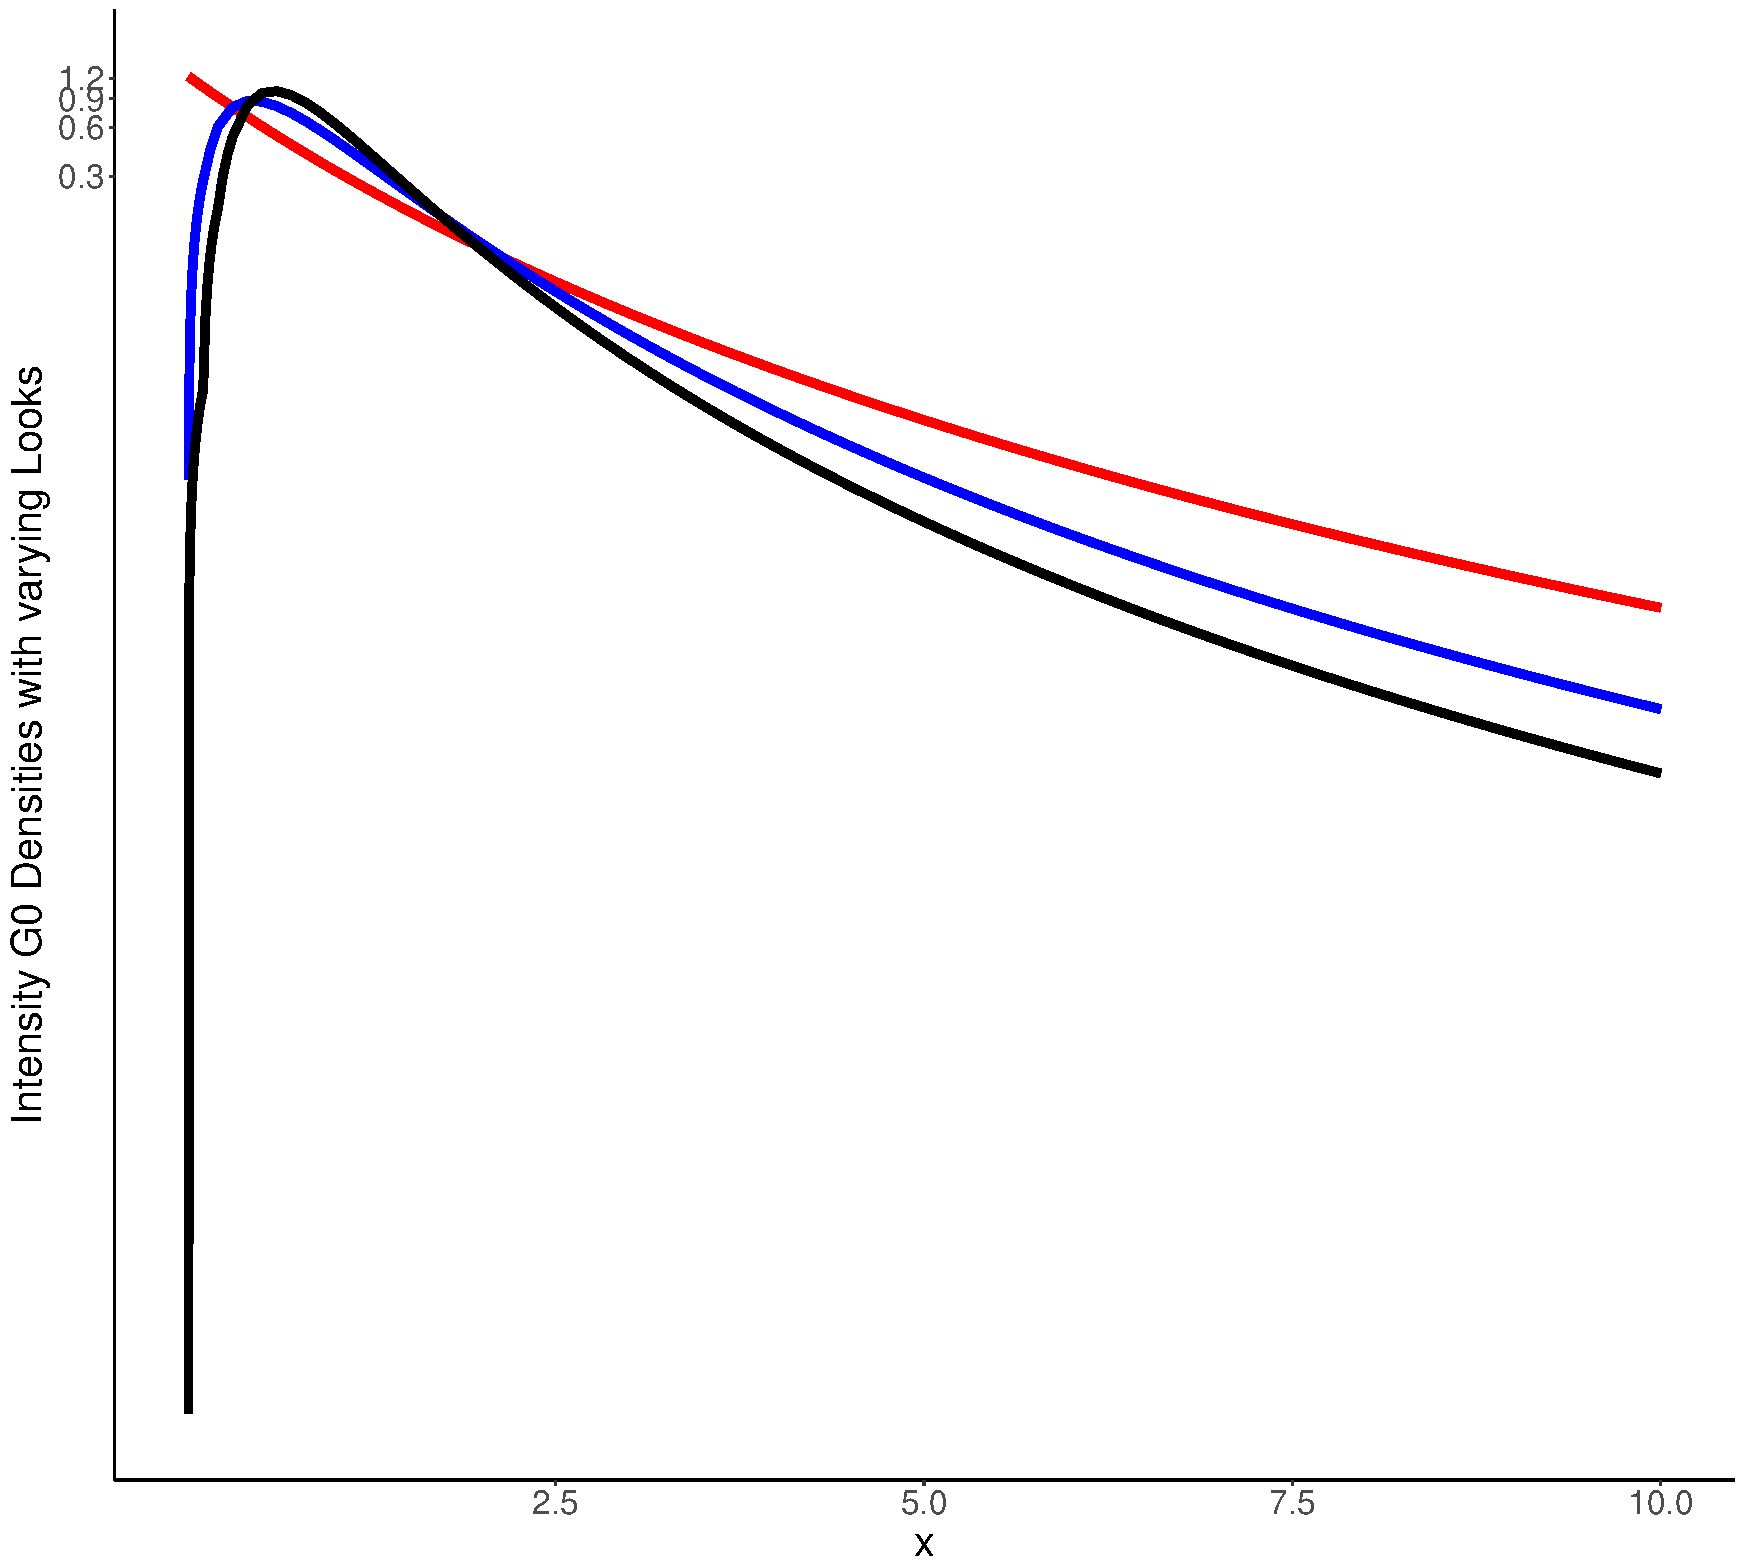
\includegraphics[width=.48\linewidth]{GI0DensitiesSemilogLooks}}
\caption[Densities in linear and semilogarithmic scale $\mathcal G^0(-5,4,L)$ distributions with unitary mean and $L\in\{1,3,8\}$]{Densities in linear and semilogarithmic scale $\mathcal G^0(-5,4,L)$ distributions with unitary mean and $L\in\{1,3,8\}$ in red, blue, and black, resp.)}\label{Fig:GI0DistributionLooks}
\end{figure}

The $\mathcal{G}^0$ distribution has the same number of parameters as the $\mathcal{K}$ law, but it has been shown to be more apt at modeling return with extreme variability.
Moreover, it is also able to describe the same kind of return from textured areas for which the latter was proposed; \citet{MejailJacoboFreryBustos:IJRS} showed that, with proper choices of parameters, the $\mathcal G^0$ law can approximate with any error any $\mathcal K$ distribution.
For these reasons, the $\mathcal G^0$ distribution is called \textit{Universal Model} for SAR data; see Exercise~\ref{Ex:ApproximationKGI0}.

The $\mathcal G^0$ distribution relates to the well-known Fisher-Snedekor law in the following manner:
\begin{equation}
F_{G^0(\alpha,\gamma,L)}(t) = \Upsilon_{2L,- 2\alpha}(- \alpha t/\gamma),
\end{equation}
where $\Upsilon_{u,v}$ is the cumulative distribution function of a Fisher-Snedekor distribution with $u$ and $v$ degrees of freedom, and $F_{G^0(\alpha,\gamma,L)}$ is the cumulative distribution function of a $F_{G^0(\alpha,\gamma,L)}$ random variable.
Notice that $\Upsilon$ is readily available in most software platforms for statistical computing.
Since such platforms usually also provide implementations of the inverse of cumulative distribution functions, the Inversion Theorem can be used to sample from the $\mathcal G^0$ law.

Arguably, the most popular way of sampling from the $\mathcal G^0$ distribution is through its multiplicative nature.
Obtaining deviates from $X\sim\Gamma(1,L)$ is immediate.
In order to sample from $Y\sim\Gamma^{-1}(\alpha,\gamma)$, one may use the fact that if $Y'\sim\Gamma(-\alpha,\gamma)$, then $Y=1/Y'$ has $\Gamma^{-1}(\alpha,\gamma)$ distribution.
Then, $Z=X/Y'$ has the desired $\mathcal G^0(\alpha,\gamma,L)$ distribution.

\citet{SamplingfromtheGI0Distribution2018} discuss other techniques for obtaining such deviates, in particular interesting connections between the $\mathcal G^0(\alpha,\gamma,1)$ law and certain Pareto distribution.

\section{Connection between Models}

\section*{Exercises}

\begin{exer}
Using~\eqref{Eq:MomentKI}, compute the skewness and kurtosis of the $\mathcal K(\alpha,\lambda,L)$ distribution.
Illustrate how they vary with the parameters.
\end{exer}

\begin{exer}
Illustrate the dependence of the density of the $\mathcal K$ distribution with respect to the scale parameter $\lambda$.
\end{exer}

\begin{exer}
Obtain samples from iid $\mathcal{K}(\alpha,\lambda,L)$ random variables.
Produce histograms, and draw the theoretical densities over them for a variety of parameters.
\end{exer}

\begin{exer}
Obtain the expression of the density of $\mathcal K$-distributed amplitude data via the transformation $Z_A=\sqrt{Z_I}$.
Compute its moments.
Illustrate.
\end{exer}

\begin{exer}
Using~\eqref{Eq:MomentGI0}, compute the skewness and kurtosis of the $\mathcal G^0(\alpha,\gamma,L)$ distribution.
Illustrate how they vary with the parameters.
\end{exer}

\begin{exer}
Illustrate the dependence of the density of the $\mathcal G^0$ distribution with respect to the scale parameter $\gamma$.
\end{exer}

\begin{exer}
Obtain samples from iid $\mathcal{G}^0(\alpha,\gamma,L)$ random variables.
Produce histograms, and draw the theoretical densities over them for a variety of parameters.
\end{exer}

\begin{exer}
Obtain the expression of the density of $\mathcal G^0$-distributed amplitude data via the transformation $Z_A=\sqrt{Z_I}$.
Compute its moments.
Illustrate.
\end{exer}

\begin{exer}
Consider~\eqref{Eq:DensKI} and~\eqref{Eq:MomentKI}.
Compute $\mu$, the expected value, from the latter, and reparametrize the former using $\mu$, $\alpha$, and $L$.
\end{exer}

\begin{exer}
Consider~\eqref{Eq:DensGI0} and~\eqref{Eq:MomentGI0}.
Compute $\mu$, the expected value, from the latter, and reparametrize the former using $\mu$, $\alpha$, and $L$.
\end{exer}

\begin{exer}\label{Ex:ApproximationKGI0}
Propose a measure of the difference between $Z_1\sim\mathcal K(\alpha_1,\lambda^*, L)$ and $Z_2\sim\mathcal G^0(\alpha_2,\gamma^*, L)$ (consider, for instance, the Hellinger distance between distributions with positive support $d_{\text{H}}(Z_1,Z_2)=1-\int_{\mathbbm R_+}\sqrt{f_{Z_1} f_{Z_2}})$.
Describe this difference for a number of values of $\alpha_1$ and $\alpha_2$, for $L\in\{1,3,8\}$.
For each $\alpha_1$, find the value of $\alpha_2$ which yields the closest $\mathcal K$ and $\mathcal G^0$ random variables\cite{mejailfreryjacobobustos2001}.
\end{exer}

\chapter{Descriptive Statistics and Visualization}\label{Chapter:DescriptiveVisualization}

\newthought{This chapter} presents two closely related sets of operations:
descriptive statistics and visualization.
The former aims at extracting valuable information, both numerical and graphical, with the least possible hypotheses about the data.
The latter gathers techniques for presenting the data as images which reveal interesting features about the scene under analysis.

\section{Descriptive Statistics}

Bearing in mind the strong connection SAR data have with their statistical properties, it is highly recommended to start handling such data as a sample. This section presents the main tools every SAR data analyst should be comfortable to use and exploit.

We will use two data sets: \texttt{dark.Rdata} and \texttt{bright.Rdata}, which were extracted from the image shown in Fig.~\ref{Im:Oberpfaffenhofen_RGB} (page~\pageref{Im:Oberpfaffenhofen_RGB}, the yellow and red areas, respectively).
Each data set is comprised of three bands: HH, HV and VV.

The first operation should always consist in checking the size and type of data:
\begin{lstlisting}
> dim(dark)
[1]  63 247   3
> typeof(dark)
[1] "double"
\end{lstlisting}
With this we know the data is arranged in three bands of \num{63} lines and \num{247} columns each, and that these are double precision floating records.

It is convenient to organize the data as a \texttt{data.frame}
\begin{lstlisting}
dark_data.frame <- data.frame(HH=as.vector(dark[,,1]),
 HV=as.vector(dark[,,2]), 
 VV=as.vector(dark[,,3]))
\end{lstlisting}

And now we can apply the \texttt{summary} function:
\begin{lstlisting}[caption={Summary statistics},label=Code:SummaryStatistics]
> summary(dark_data.frame)
             HH                  HV                  VV
 Min.   :     1   Min.   :    0.004   Min.   :     0.17  
 1st Qu.:  1821   1st Qu.:  134.675   1st Qu.:   950.78  
 Median :  4414   Median :  326.652   Median :  2364.09  
 Mean   :  7552   Mean   :  509.596   Mean   :  3882.10  
 3rd Qu.:  9060   3rd Qu.:  662.560   3rd Qu.:  4957.64  
 Max.   :526287   Max.   :15723.672   Max.   :134204.69  
\end{lstlisting}

We immediately notice the different ranges: the observations in the HV band are one order of magnitude smaller than those in the other bands.

The histograms of these bands were shown in Fig.~\ref{Fig:FittedDarkRegion}.
Another useful representation of the marginal distribution of the data is the boxplot.

A boxplot is a graphical representation of the marginal properties of the data.
It depicts the median, the lower and upper quartiles, and possible outliers.
It may also contain notches that represent approximate interval confidence for the median.

In order to draw boxplots using our library of choice \texttt{ggplot2}, we need to ``melt'' the data frame structure.
The listing below produces Fig.~\ref{Fig:BoxplotDark}, in semilogarithmic scale.

\begin{lstlisting}
dark_DF <- melt(dark_data.frame)
ggplot(dark_DF, aes(x=variable, y=value)) + 
  geom_boxplot(notch = TRUE) + 
  coord_trans(y="log") + 
  xlab("Bands") +
  ylab("Observations in Logarithmic Scale") + 
  theme_few() +
  theme(text = element_text(size=20))
\end{lstlisting}

\begin{figure}
\centering
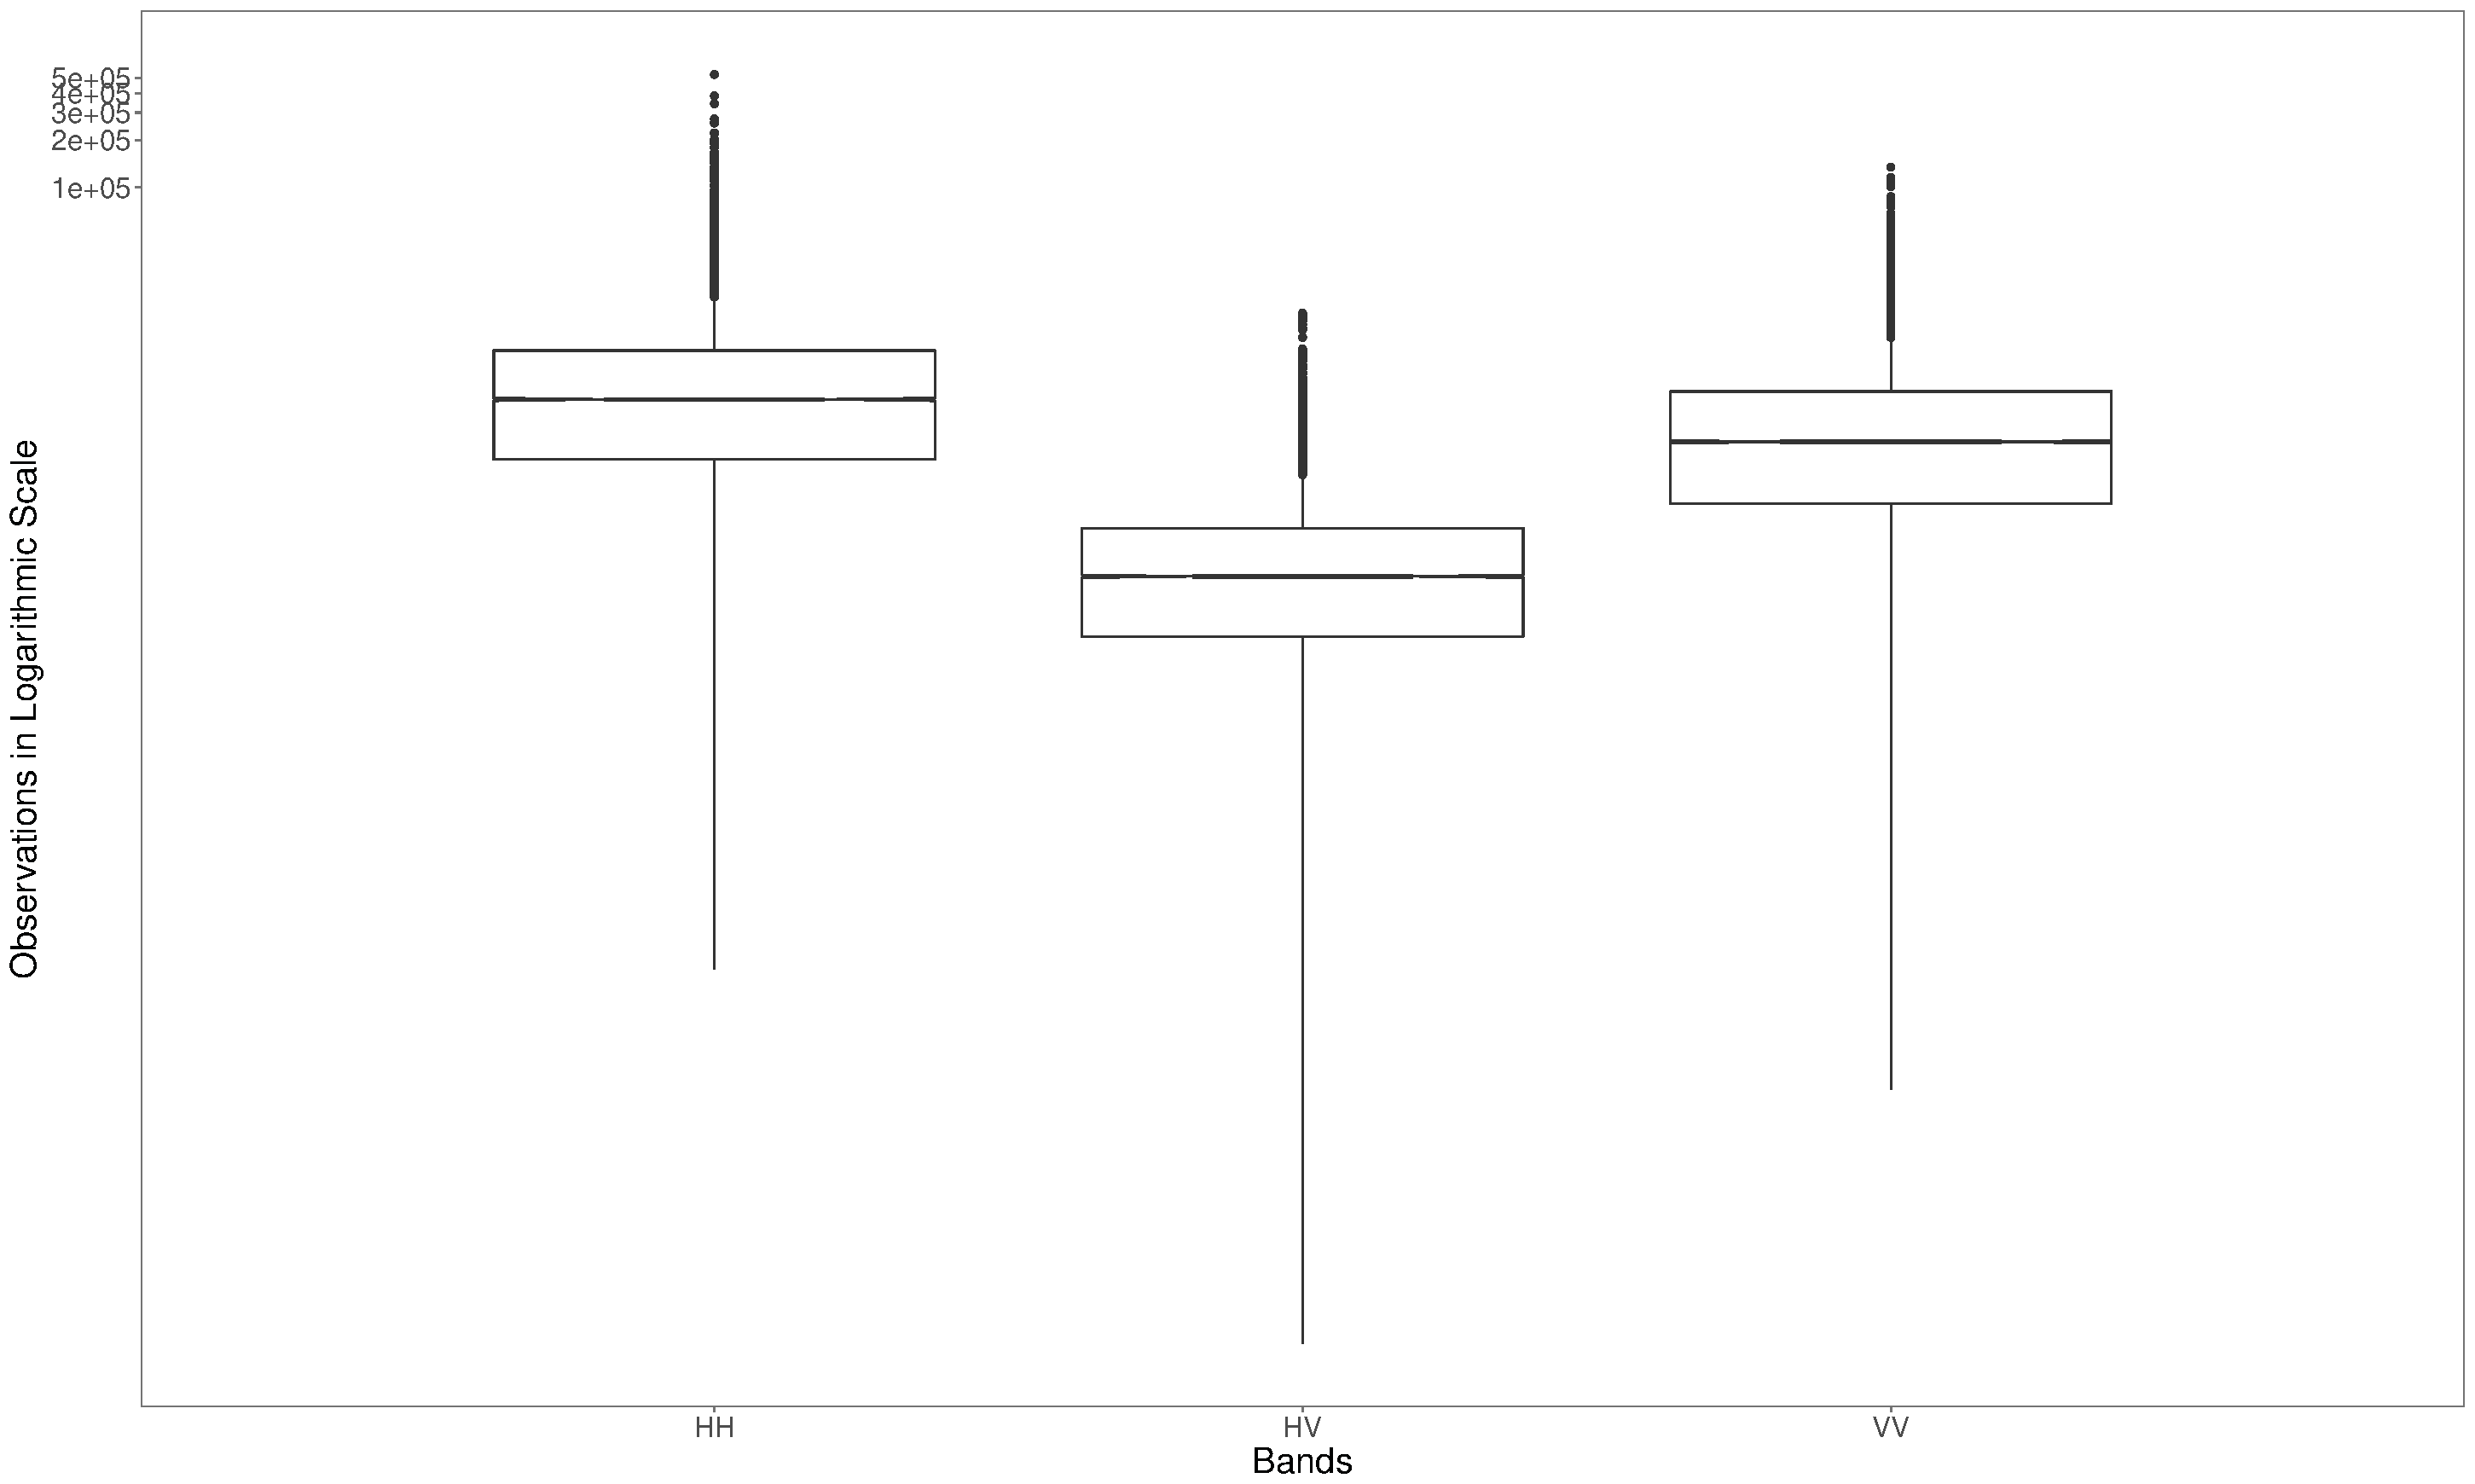
\includegraphics[width=\linewidth]{BoxPlotdark}
\caption{Boxplot of the three bands from the \texttt{dark} image}\label{Fig:BoxplotDark}
\end{figure}

Fig.~\ref{Fig:BoxplotDark} depicts what the \texttt{summary} command had revealed already, but it also provides strong evidence in favor of highly skewed data.
We were aware of this from Fig.~\ref{Fig:FittedDarkRegion}.
The notches are barely visible due to the large sample size.

\section{Visualization}

Image visualization is the operation that maps values into pixels\cite{IPVG:2008}.
This mapping may be to a screen or to a file.

SAR images often have a huge dynamic range.
\chapter{Parameter Estimation}\label{Chapter:ParameterEstimation}

\newthought{At this point} we have data and models.
We will see ways of using the former to make inferences about the latter.

Assume we have a parametric model $(\Omega, \mathcal A, \Pr)$ for real independent random  variables $X$ and $\bm X = (X_1,X_2,\dots)$.
The distribution of $X$ is indexed by $\bm \theta\in\bm \Theta\subset \mathbbm R^p$, where $p\geq 1$ is the dimension of the parametric space $\bm \Theta$.

What can we say about $\bm \theta$ using the sample $\bm X$?
This is parametric statistical inference!

We will later need an additional ingredient: expected values of transformations of the random variable $X$:
\begin{equation}
\operatorname{E}\bm\psi(X) = \big(
\operatorname{E}\psi_1(X), \operatorname{E}\psi_2(X), \dots, \operatorname{E}\psi_p(X)
\big),
\label{eq:ExpectedValues}
\end{equation}
where each $\psi_j$ is a measurable function $\psi_j\colon \mathbbm R\to\mathbbm R$.
Each element of~\eqref{eq:ExpectedValues} is given by
\begin{equation}
\operatorname{E}\psi_j(X) = 
	\int_{\mathbbm R} \psi_j(x) dF(x),
\end{equation}
and $F$ is the cumulative distribution function of $X$.
If $\psi(X)=X^k$, we say that $\operatorname{E}X^k$ is the $k$-th order moment of $X$ (if it exists).

The quantity $\operatorname{E}(X-\operatorname{E}X)^k$ is called ``the central moment'' of $X$, if it exists.
The second central moment $\operatorname{E}(X-\operatorname{E}X)^2 = \operatorname{E}X^2-(\operatorname{E}X)^2$ is called ``the variance'' of $X$.
We denote it $\operatorname{Var}X$

In general, $\operatorname{E}X^k\neq (\operatorname{E}X)^k$.

\section{Models}

We will use a few models as examples.
The interested reader is referred to, among other references, to the books by \citet{johnson_discrete} for discrete distributions, and by \citet{johnson_continuous2} for continuous random variables.

\subsection{The Bernoulli distribution}\label{Sec:Bernoulli}

This is the basic discrete distribution.
It models the outcome of a dichotomic random experiment, i.e., with only two possible outcomes: failure ($0$) or success ($1$).
Denote $N\sim\text{Be}(p)$ a random variable with Bernoulli distribution and probability $0\leq p\leq 1$.
The vector of probabilities is $(1-p,p)$.

\subsection{The Negative Binomial distribution}\label{Sec:NegativeBinomial}

This discrete distribution is basilar in the construction of the $\mathcal K$ law.
We say that $N\sim\text{NB}(r,p)$ has negative binomial distribution if its vector of probabilities is given by
$$
\Pr(N=n) = {{k+r-1}\choose{k}} p^k (1-p)^r,
$$
com $0<p<1$ and $1\leq n\leq k$.

This is the distribution that models the probability of having to wait until the $n$th Bernoulli trial with probability $p$ of success until we observe exactly $r$ failures.

\subsection{The Uniform distribution}\label{Sec:UnifDistribution}

We say that $X\sim\mathcal U_{(0,\theta)}$, $\theta>0$ has uniform distribution on the interval $(0,\theta)$ when its density is
\begin{equation}
f_U(u;\theta) = \frac{1}{\theta} \mathbbm 1_{(0,\theta)} (u).
\label{eq:DensUniform}
\end{equation}
With this, we have that the $k$-order moment of $X$ is
\begin{equation}
\operatorname{E}U^k = \int_{\mathbbm R}\frac{1}{\theta} \mathbbm 1_{(0,\theta)} u^k d(u) du = 
\int_{0}^{\theta} \frac1\theta u^k du = 
\frac{1}{k+1} \theta^k.
\label{eq:MomentsUniform}
\end{equation}

Its cumulative distribution function is
\begin{equation}
F_U(u;\theta) = 
	\begin{cases}
	0 				& \text{if } u\leq 0,\\
	u/\theta 	& \text{if } 0< u < \theta,\\
	1 				& \text{otherwise.}
	\end{cases}
\label{eq:CDFUniform}
\end{equation}

\subsection{The Gaussian distribution}

We say that $X\sim N(\mu,\sigma^2)$ follows a Gaussian distribution with mean $\mu\in\mathbbm R$ and variance $\sigma^2$ if the density that characterizes its distribution is
\begin{equation}
f_G(x;\mu,\sigma^2) = \frac{1}{\sqrt{2\pi}\sigma} \exp\Big\{
-\frac{1}{2\sigma^2} \big(x - \mu)^2
\Big\}.
\end{equation}
Its first and second moment are $\operatorname{E}X=\mu$ and
$\operatorname{E}X^2=\mu^2+\sigma^2$.

We don't know explicit expressions for its cumulative distribution function, but it is widely implemented in almost every statistical platform.

\subsection{Mixture of Gaussian distributions}

A mixture of $p$ Gaussian models is characterized by the density
\begin{equation}
f_{\text{MG}}(x;\bm p,\bm \mu, \bm \sigma^2) = 
\sum_{j=1}^{p}
\frac{p_j}{\sqrt{2\pi}\sigma_j} \exp\Big\{
-\frac{1}{2\sigma_j^2} \big(x - \mu_j)^2 \Big\},
\label{eq:DensMixtureGaussian}
\end{equation}
where $\bm p=(p_1,p_2, \dots, p_p)$ is the vector of probabilities,
$\bm \mu = (\mu_1, \mu_2,\dots, \mu_p)$ is the vector of means,
and
$\bm \sigma^2 = (\sigma^2_1, \sigma^2_2,\dots, \sigma^2_ p)$ is the vector of variances.
In this way, the parameter space is $\bm \Theta =
\mathcal S^p\times \mathbbm R^p \times \mathbbm R_+^p$, where
$\mathcal S^p$ is the surface of the $p$-dimensional simplex.
This space is a subset of $\mathbbm R^{(p-1)p^2}$. 
We denote this situation $X\sim \text{MG}(\bm p, \bm \mu, \bm \sigma^2)$.

Using the fact that the random components are independent, it is immediate that
$\operatorname{E}X = \sum_{j=1}^{p} p_j\mu_j$ and that
$\operatorname{Var}X = \sum_{j=1}^{p} p_j^2\sigma^2_j$.

\subsection{The (SAR) Gamma distribution}

The Gamma distribution, in the usual parametrization for SAR data $Z\sim\Gamma(L,\mu)$, with $L,\mu>0$ is characterized by the density
\begin{equation}
f_\Gamma(z;L,\mu) = \frac{L^L}{\mu^{L}\Gamma(L)} z^{L-1} 
	\exp\big\{ -L z / \mu
	\big\}.
\label{eq:SARGammaDensity}
\end{equation}
With this, the first- and second-order moments of $Z$ are
$\operatorname{E}Z=\mu$,
and 
$\operatorname{Var}Z=\mu^2/L$,
respectively.

As for the Gaussian distribution, in general, we do not have explicit expressions for its cumulative distribution function, being the exponential case ($L=1$) an exception.

This is a good model for intensity SAR observations over areas with no texture.
The multiplicative model says the observed return $Z$ is the product of two independent random variables:
$X$, the backscatter, and
$Y$, the speckle.
The speckle can be modeled by a Gamma random variable with shape parameter $L\geq1$ (the number of looks) and unitary mean.

If the area under observation has constant backscatter ($X=\mu$), then the return $Z\sim\Gamma(\mu,L)$.

\subsection{The Reciprocal Gamma distribution}

When the backscatter varies in the observed area we say that the area has texture.
A very flexible model for the backscatter is the Reciprocal Gamma law\cite{frery96}, which is characterized by the density
\begin{equation}
f_Y(y;\alpha,\gamma)= \frac{1}{\gamma^\alpha \Gamma(\alpha)}
y^\alpha \exp\big\{-\gamma/y\big\},
\label{eq:IGDensity}
\end{equation}
where $\alpha<0$ is the texture, and
$\gamma>0$ is the scale.
We denote this situation $Y\sim \Gamma^{-1}(\alpha,\gamma)$.

\subsection{The GI0 distribution}

Assuming that the backscatter is $X\sim\Gamma^{-1}(\alpha,\gamma)$,
the speckle is $Y\sim\Gamma(1,L)$, and that they are independent random variables, we have that the return follows a GI0 distribution\cite{GeodesicDistanceGI0JSTARS,ParameterEstimationSARStochasticDistancesKernels}, denoted $Z\sim\mathcal G_I^0(\alpha,\gamma,L)$, whose density is
\begin{equation}
f_Z(z;\alpha,\gamma,L) = \frac{L^L \Gamma(L-\alpha)}{\gamma^\alpha \Gamma(L) \Gamma(\alpha)}
\frac{z^L}{(\gamma+Lz)^\alpha}.
\end{equation}

The $k$-order moment of $Z$ is given by
\begin{equation}
\operatorname{E}Z^k = \Big(\frac{\gamma}{L}\Big)^k
\frac{\Gamma(-\alpha-k)}{\Gamma(-\alpha)}
\frac{\Gamma(L+k)}{\Gamma(L)},
\end{equation}
provided $k>-\alpha$ and infinite otherwise.

\section{Inference by analogy}

Inference by analogy\cite{manski_analog} is inspired by the Law of Large Numbers, that states that (under relatively mild conditions) holds that
\begin{equation}
\lim_{n\to\infty}\frac1n\sum_{i=1}^{n} \psi(X_i) = 
\operatorname{E}\psi(X),
\label{eq:LLN}
\end{equation}
provided $X,X_1,X_2,\dots$ are independent identically distributed random variables.

With this in mind, and assuming one has a large sample, it seems reasonable to equate sample quantities (the left hand side) and parametric expressions (the right hand side).

When we have $p$ parameters, i.e. $\bm \theta\in\Theta\subset\mathbbm R^p$, we need $p$ linearly independent equations to form an estimator of $\bm \theta$.

\subsection{The Uniform distribution}

Using~\eqref{eq:MomentsUniform} with we can set, for instance, $k=1$ and obtain $\operatorname{E}U=\theta/2$.
With this, our first-order moment estimator for $\theta$ is $\widehat{\theta}_1=2n^{-1}\sum_{i=1}^n U_i$.
But we can also set $k=2$ and obtain a second-order moment estimator, using $\operatorname{E}U^2=\theta^3$ it is immediate that
$\widehat{\theta}_2=\sqrt{3n^{-1}\sum_{i=1}^{n} U_i^2}$.
In fact, the $k$-order moment estimator of $\theta$ based on a sample of size $n$ is
\begin{equation}
\widehat{\theta}_k = \sqrt[k]{\frac{k+1}{n} \sum_{i=1}^{n} U_i^k}.
\end{equation}

This multiplicity of possible analogy estimators gives great flexibility to the method, but it is also one of its weaknesses: the lack of unicity.
Another drawback is that little is known about estimators obtained by this procedure, apart that they are consistent, i.e., that~\eqref{eq:LLN} grants that they converge in probability to the true parameter value.

A more serious problem is that an estimator obtained by this procedure may lead to a model for which observations are unfeasible (and, remember, observations are \emph{correct}).
See, for example, the sample $\bm x=(0.05, 0.15, 1)$.
Its sample mean is $1.2/3=0.4$, therefore the estimate is $\widehat{\theta}_1=0.8$, but the third observation is unfeasible under the $\mathcal U_{(0,0.8)}$ distribution!

By the way, notice an important difference.
We refer to an \emph{estimator} when it is a random variable $\widehat{\theta}(X_1, X_2, \dots)$, and to an \emph{estimate} when the data have been observed $\widehat{\theta}(x_1, x_2, \dots)$ and, thus, is a fixed quantity.

\subsection{The Gaussian distribution}

Using $\operatorname{E}X=\mu$ we obtain $\widehat{\mu}=n^{-1}\sum_{i=1}^{n} X_i$.
Since $\operatorname{E}X^2=\mu^2+\sigma^2$, we have that $\sigma^2=\operatorname{E}X^2-\mu^2$.
We already have an estimator for $\mu$, and also for $\mu^2$, then one estimator for $\sigma^2$ is $\widehat{\sigma}^2=n^{-1}\sum_{i=1}^{n}X_i^2-\widehat{\mu}^2 = n^{-1}\sum_{i=1}^{n}(X_i-\widehat{\mu})^2$.

Other estimators could be formed with higher-order moments $k=3,4\dots$, but we will always need two linearly independent equations to estimate $\bm\theta=(\mu,\sigma^2)$.

\subsection{Mixture of Gaussian distributions}

We need $(p-1)p^2$ linearly independent equations to estimate $\bm{\theta} = (\bm p, \bm \mu, \bm \sigma^2)$.
This approach is not very effective, because results in serious numerical problems.

\subsection{The (SAR) Gamma distribution}

Using $\E(Z)=\mu$ we propose $\widehat{\mu}=n^{-1}\sum_{i=1}^n Z_i$,
and with 
$\operatorname{Var}(Z)=\mu^2/L$, we can estimate $\widehat L=\widehat{\mu}^2 / (n^{-1}\sum_{i=1}^n (Z_i - \widehat{\mu})^2)$.
This is the well-now estimator for the number of looks (equivalent number of looks) which consists of the reciprocal of the squared coefficient of variation.

\section{Inference by maximum likelihood}

The principle of likelihood was formalized by R.\ A.\ Fisher.
In most practical situations it produces unique estimators, and has good and well-known properties.
It should be used whenever possible.

Consider again the sample independent of random variables $\bm = (X_1,X_2,\dots,X_n)$ each with the same distribution characterized (without lack of generality) by the density $f(X_i;\bm \theta)$.
The likelihood function is
\begin{equation}
\mathcal L(\bm \theta;\bm X) = \prod_{i=1}^{n} f(\bm \theta;X_i).
\label{eq:Likelihood}
\end{equation}
Notice that $\mathcal L$ is not a joint density function, as it depends on $\bm \theta$, not on the variables.

The principle of maximum likelihood proposes as estimator for $\bm \theta$ the parameter that maximizes~\eqref{eq:Likelihood}:
\begin{equation}
\widehat{\bm \theta}_{\text{ML}} = \arg\max_{\bm\theta\in\bm{\Theta}}
\Big\{ \mathcal L(\bm \theta;\bm X)
\Big\},
\end{equation}
that is, the point in $\bm \Theta$ that makes the observations most plausible.
It sometimes coincides with some analogy estimators.

\subsection{The Uniform distribution}

Assume $\bm U=(U_1,U_2,\dots, U_n)$ is a sample from $\mathcal U_{(0,\theta)}$, with $\theta>0$ unknown.
The likelihood is
\begin{equation}
\mathcal L(\bm \theta;\bm U) = \prod_{i=1}^{n} \frac1\theta \mathbbm 1_{(U_i,\infty)}(\theta).
\label{eq:LikelihoodUniform}
\end{equation}
Denote the sorted sample in nondecreasing order $U_{1:n},U_{2:n},\dots,U_{n:n}$.
After some manipulation, one arrives at the following expression:
\begin{equation}
\mathcal L(\bm \theta;\bm U) = \frac1{\theta^n} \mathbbm 1_{(U_{n:n},\infty)} (\theta),
\label{eq:LikelihoodUniformReady}
\end{equation}
whose maximum is at $U_{n:n}$, so 
$\widehat{\theta}_{\text{ML}}=\max \{U_1,U_2,\dots,U_n\}$.

This is quite different from any analogy estimator, and the estimator by maximum likelihood is always admissible.

\subsection{Beta distribution}\label{Sec:BetaDistribution}

Closely related to the Uniform distribution is the Beta law\cite{devro86}.
We say that $B$ follows a Beta distribution with shape parameters $a,b>0$ if its density is given by
\begin{equation}
f_B(u;p,q) = \frac{\Gamma(a+b)}{\Gamma(a)\Gamma(b)} u^{a-1} (1-u)^{b-1} \mathbbm 1_{(0,1)} (u).
	\label{eq:BetaDensity}
\end{equation}
We denote this situation as $B\sim\mathcal B(a,b)$.
Its expected value and variance are given by:
$$
\operatorname{E}(B) = \frac{a}{a+b} \text{ and }
\operatorname{Var}(B) = \frac{ab}{(a+b)^2(a+b+1)}.
$$

It is noteworthy that $\mathcal B(1,1)$ is the Uniform distribution, and that if $a=b$ the density is symmetric around $1/2$.
If $a=b>1$ the unique mode is at $1/2$, otherwise there are two modes at $0$ and $1$.
Fig.~\ref{Fig:BetaDensities} illustrates three of these situations.

\begin{marginfigure}
\centering
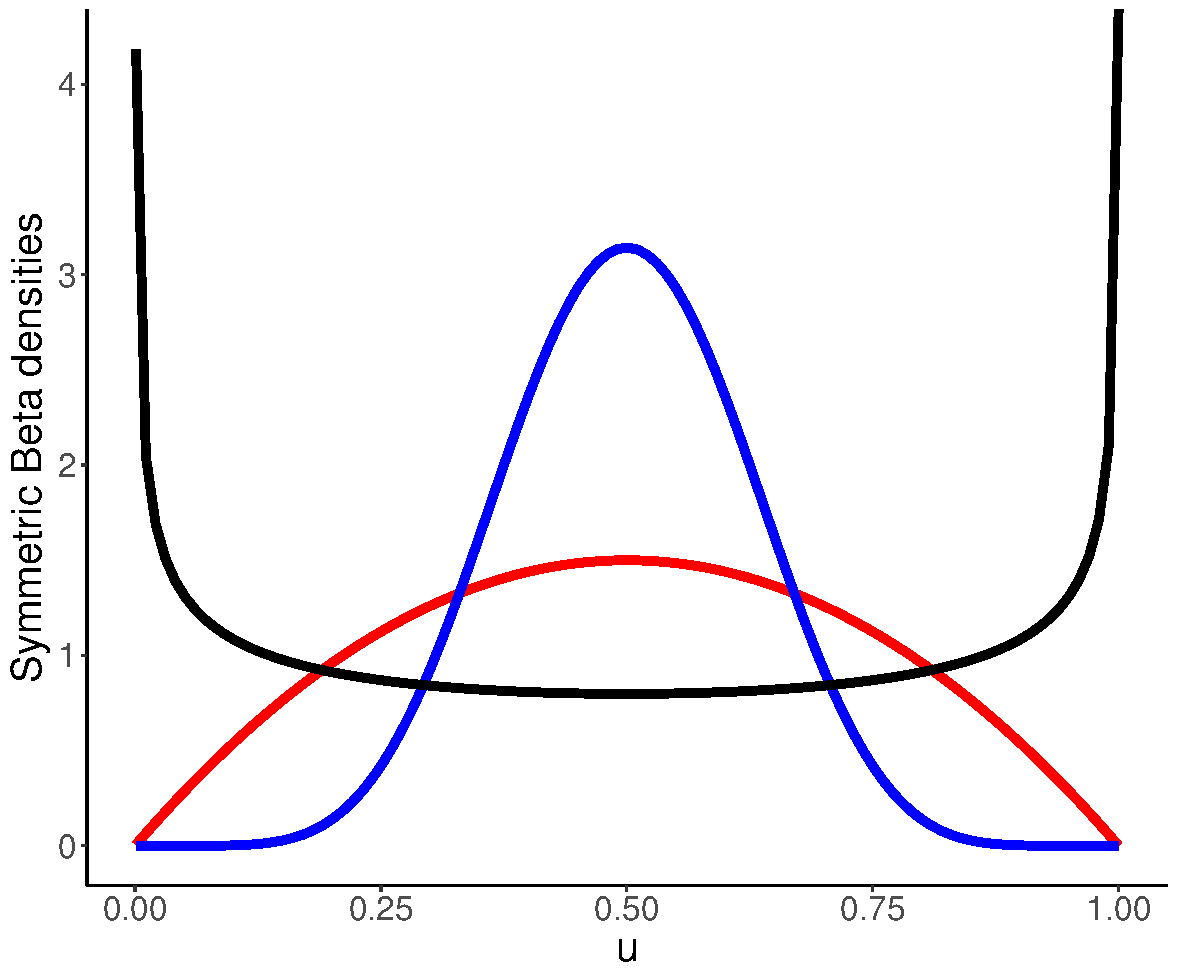
\includegraphics[width=\linewidth]{SymmetricBetaDensities}
\caption{Beta densities with $a=b\in \{0.7,2,8 \}$ (black, red, blue).}
\label{Fig:BetaDensities}
\end{marginfigure}

\subsection{The Gaussian distribution}

In this case, $\widehat{\bm\theta}_{\text{ML}}$ coincides with the analogy estimators we already derived using analogy.

\subsection{Mixture of Gaussian distributions}

The ML estimator poses a difficult optimization problem.
It consists of finding
\begin{equation}
\widehat{(\bm p,\mu,\sigma^2)}_{\text{ML}} = \arg\max_{(\bm p,\mu,\sigma^2)\in\bm{\Theta}}
\sum_{j=1}^{p}
\frac{1}{\sqrt{2\pi}\sigma_j} \exp\Big\{
-\frac{1}{2\sigma_j^2} \big(x - \mu_j)^2 \Big\}.
\end{equation}
This is so difficult and numerically unstable, that it is often solved by using the EM (Expectation-Maximization) algorithm.
It is highly recommended to use the \texttt{mclust} package\cite{mclust4} available in \texttt{R}\cite{Rmanual}.

Since we assume no knowledge about the number of components $p$, it is important to use a balance between the number of parameters and the likelihood, otherwise we may end with a model with the largest possible $p$.

There are many measures of the quality of models, among them BIC -- Bayesian Information Criterion, and AIC -- Akaike Information Criterion.
The latter is defined as
$$
\text{AIC} = 2\big(\#\bm\Theta - \log \mathcal L(\widehat{\bm{\theta}};\bm X)\big),
$$
and the preferred model is the one that minimizes AIC.

In the following, we will see the analysis of the \verb|rms_hist75| data set.
%We assume we are familiar with these data after performing all the steps discussed in our previous meeting.

\begin{lstlisting}[frame=lines]
require(mclust)

Cluster_rms <- Mclust(rms_hist75)

summary(Cluster_rms, parameters=TRUE)
----------------------------------------------------
Gaussian finite mixture model fitted by EM algorithm 
----------------------------------------------------

Mclust V (univariate, unequal variance) model with 5 components:

 log.likelihood     n df       BIC       ICL
      -9136.971 10628 14 -18403.74 -24127.96

Clustering table:
   1    2    3    4    5 
1621 2279 2282 2289 2157 

Mixing probabilities:
        1         2         3         4         5 
0.1411560 0.2320424 0.2117919 0.2019720 0.2130377 


Means:
        1         2         3         4         5 
0.4433623 0.8725293 1.3735809 1.7767188 2.1723729 

Variances:
         1          2          3          4          5 
0.01770870 0.05512462 0.03631520 0.03145717 0.05008409 
\end{lstlisting}

Fig.~\ref{fig:BIC} shows the values of the BIC varying with the number of components.

\begin{marginfigure}
\centering
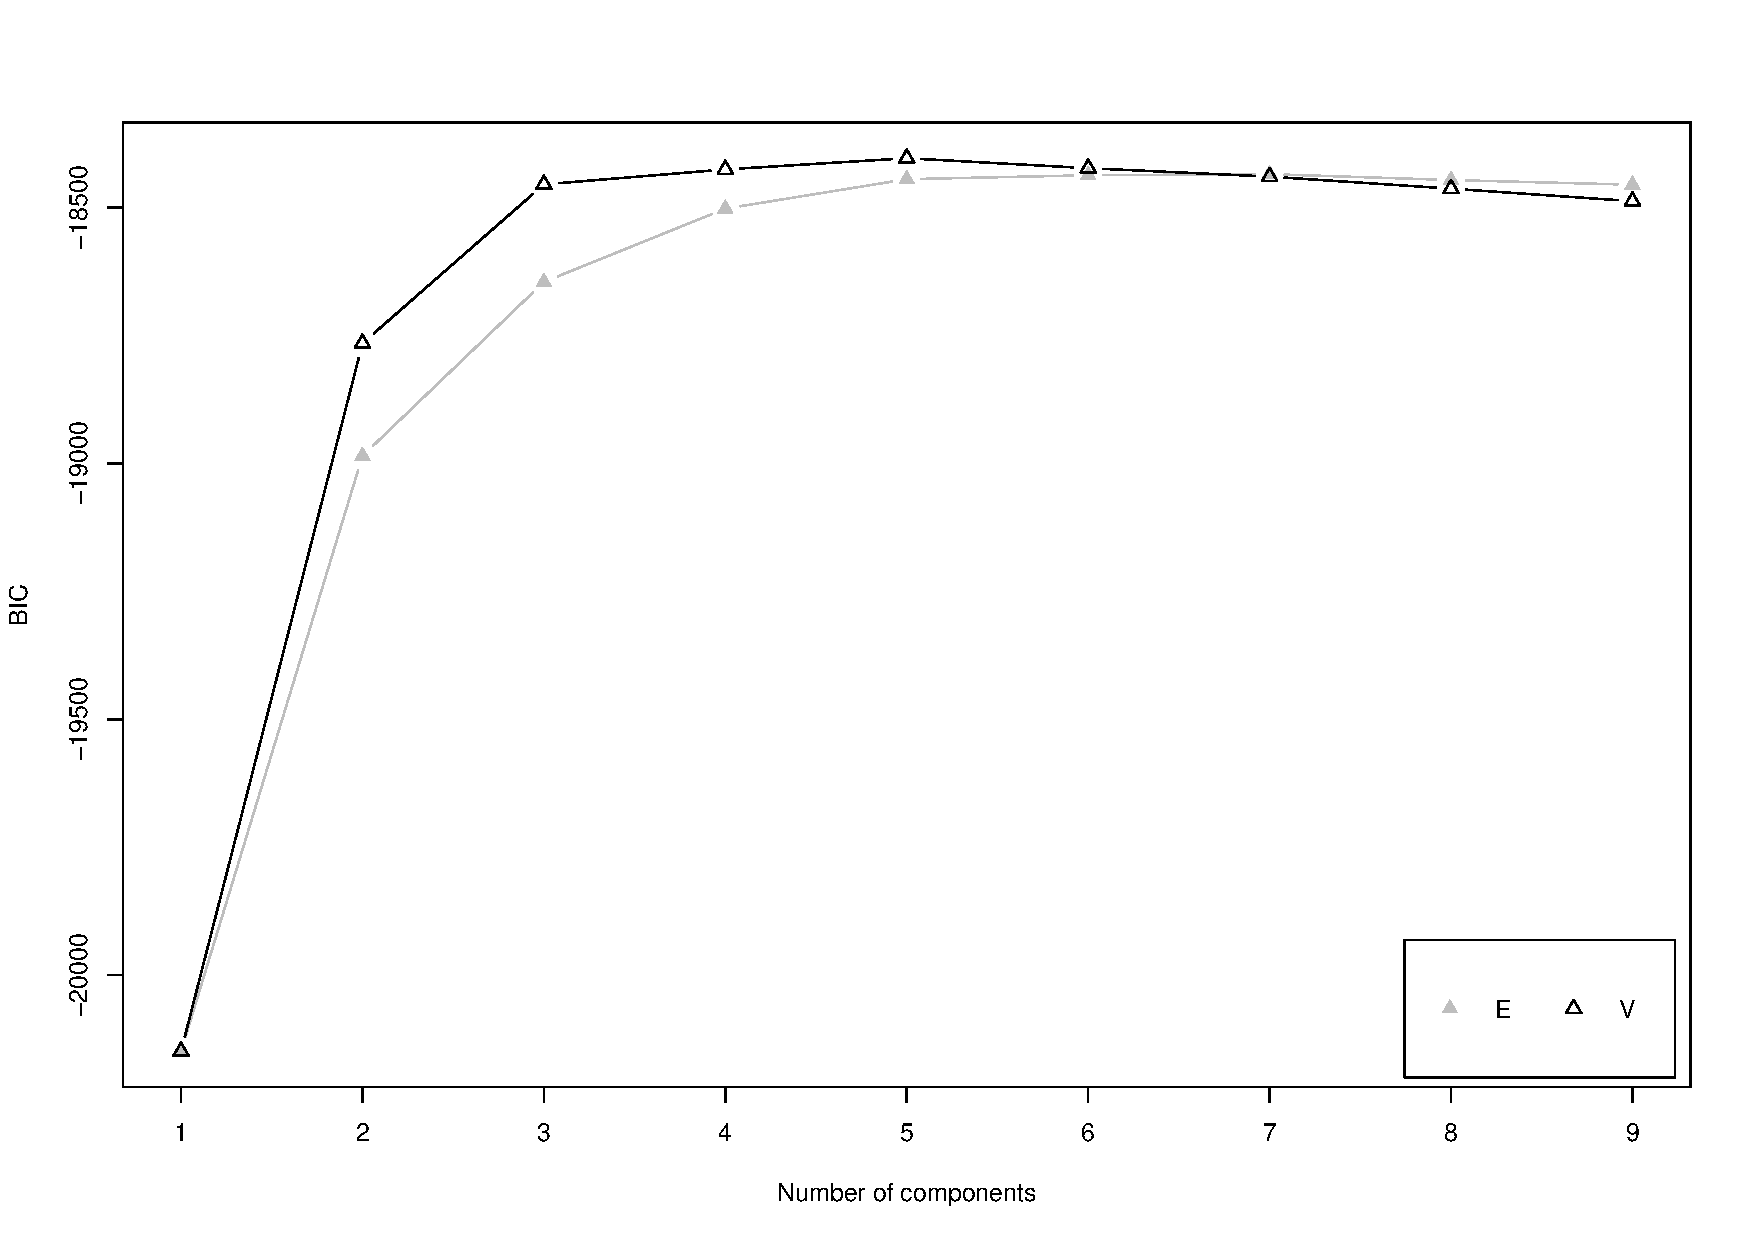
\includegraphics[width=\linewidth]{BIC}
\caption{BIC for several numbers of components}
\label{fig:BIC}
\end{marginfigure}

Fig.~\ref{fig:MixtureFit} shows the histogram, the individual components and the final model fit to the \verb|rms_hist75| data set.

\begin{marginfigure}
\centering
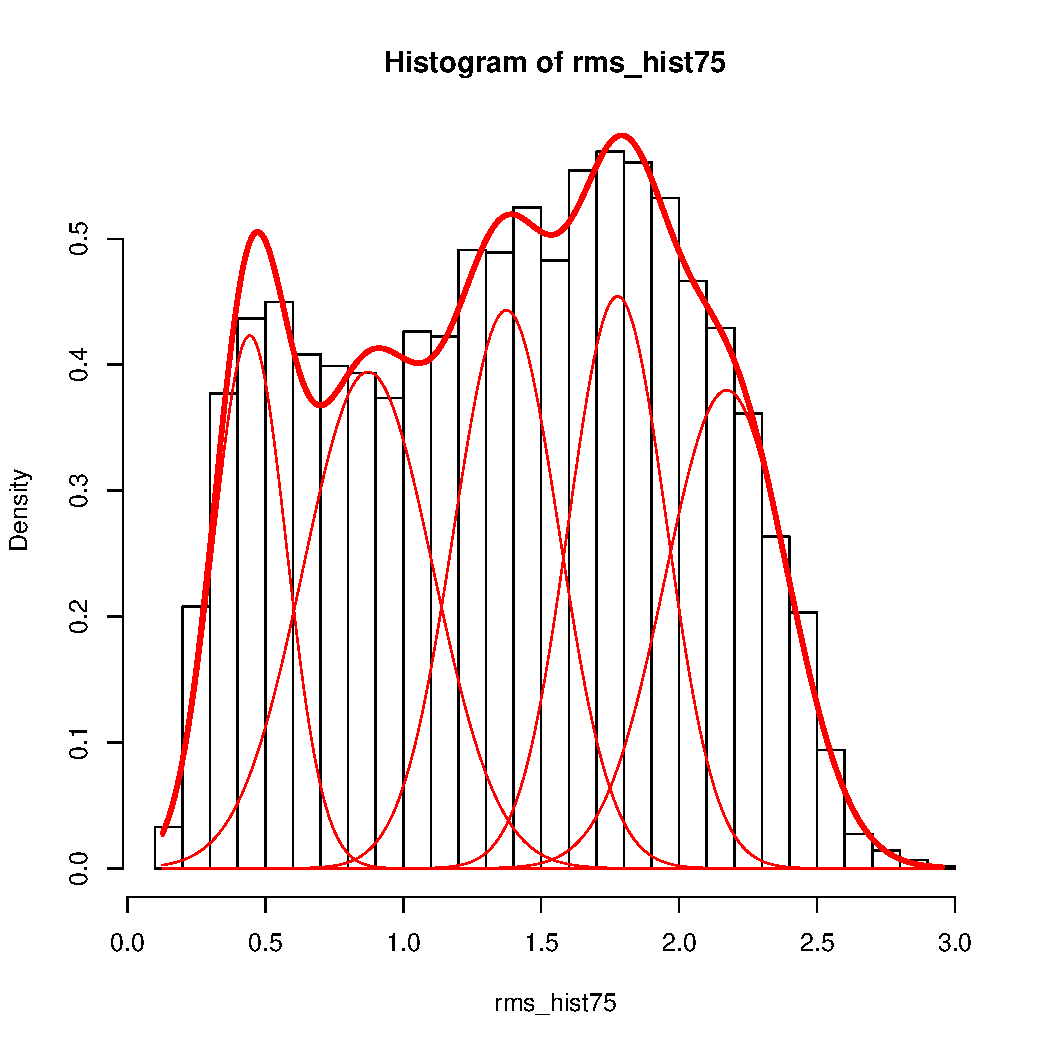
\includegraphics[width=\linewidth]{rms_hist75}
\caption{Histogram, individual components and resulting mixture model}
\label{fig:MixtureFit}
\end{marginfigure}


\subsection{The (SAR) Gamma distribution}

The likelihood function is 
\begin{align}
\mathcal L(L,\mu;\bm Z) =& \prod_{i=1}^{n}f_\Gamma(L,\mu; Z_i) = \prod_{i=1}^{n}\frac{L^L}{\mu^{L}\Gamma(L)} Z_i^{L-1} 
	\exp\big\{ -L Z_i / \mu
	\big\} \nonumber\\
	& = 
	\bigg(
	\frac{L^L}{\mu^{L}\Gamma(L)}
	\bigg)^n \prod_{i=1}^{n} \Big[Z_i^{L-1} \exp\big\{ -L Z_i / \mu
		\big\} \Big].
\end{align}
This is a very tough function to maximize.

A usual trick is taking the logarithm, as the likelihood function is positive.
One then obtains the ``complete log-likelihood function'':
\begin{equation}
\ell^*(L,\mu;\bm Z)=n\big[L(\log L - \log\mu) - \log\Gamma(L)
\big] + (L-1)\sum_{i=1}^n \log Z_i - \frac{L}{\mu} \sum_{i=1}^n Z_i.
\end{equation}
But there are terms that do not depend on either $L$ or $\mu$ and, therefore, are irrelevant for our maximization problem.
We are finally interested in the ``reduced log-likelihood function'':
\begin{equation}
\ell(L,\mu;\bm Z)=n\big[L(\log L - \log\mu) - \log\Gamma(L)
\big] + L\sum_{i=1}^n \log Z_i - \frac{L}{\mu} \sum_{i=1}^n Z_i.
\label{eq:RedLogLikGammaSAR}
\end{equation}

The maximum likelihood estimator of $(L,\mu)$ is then any point in $\mathbbm R_+^2$ satisfying
\begin{equation}
\widehat{(L,\mu)} = \arg\max_{(L,\mu)\in\mathbbm R_+^2} \ell(L,\mu;\bm Z).
\end{equation}

This problem can be solved in two ways: either deriving, equating to zero and solving, or by direct maximization.
Each case must be studied from a computational viewpoint to choose the most suitable option.

\section{The $\mathcal G^0$ distribution}

Recall that the $\mathcal G^0$ distribution was proposed as a means to model data from textured and extremely textured areas.
Assume that some textureless areas have been identified and that, with these data, it was possible to obtain a dependable estimate of $L$, say $\widehat L$.
As this equivalent number of looks should be valid for the whole image, we will consider it know when fitting data from textured areas.

Assume, then, that we have a sample $\bm Z = (Z_1,\dots,Z_n)$ of iid random variables that follow the $\mathcal G^0(\alpha,\gamma,\widehat L)$ distribution.
The unknown parameter $\theta=(\alpha,\gamma)$ lies in $\Theta=\mathbbm R_- \times \mathbbm R_+$.

The maximum likelihood estimator of $(\alpha,\gamma)$, is any point that maximizes the reduced log-likelihood:
\begin{equation}
\ell(\alpha,\gamma;\widehat L, \bm Z) = 
\frac{\Gamma(\widehat L-\alpha)}{\gamma^\alpha \Gamma(-\alpha)} +
\widehat L \sum_{n=1}^N \log\frac{Z_n}{\gamma+\widehat L Z_n} + 
\alpha \sum_{n=1}^N \log(\gamma + \widehat L Z_n),
\label{Eq:ReducedLogLikGI0}
\end{equation}
provided it lies in $\Theta$.
Maximizing~\eqref{Eq:ReducedLogLikGI0} might be a difficult task, in particular in textureless areas where $\alpha\to-\infty$ and the $\mathcal G^0$ distribution becomes very close to a Gamma law.
Small samples also pose difficult numerical problems, as $\ell$ becomes flat\cite{FreryCribariSouza:JASP:04}.

Most algorithms for maximizing~\eqref{Eq:ReducedLogLikGI0} require a starting point.
A good solution consists in using estimates obtained with the method of moments, i.e.\ by forming a system of two equations with suitable different values of $k$ in~\eqref{Eq:MomentGI0}.

\section{Analogy vs.\ Maximum Likelihood}

These methods should not be seen as competitors; they are complementary.

Analogy is usually more straightforward than Maximum Likelihood.
In particular, it does not require the expression of the density of the model (think, for instance, in the problem of estimating the parameter of the sum of $k$ random variables with $\mathcal U_{(0,\theta)}$ distribution).
Analogy leads to finding the roots of a system of (usually nonlinear) equations, and this is usually cumbersome in high-dimensional parametric spaces.

Estimators derived by Maximum likelihood have many asymptotic properties, and they are regarded to as the best ones for large samples when there is no contamination.
They can be obtained by either finding the roots of a system of (again, usually nonlinear) equations, which shares the problems of Analogy, or by optimization of the reduced log-likelihood function.
There are a number of excellent algorithms for the latter approach, numerical optimization\cite{maxLik}, EM and Simulated Annealing among them.

One frequently uses an analogy estimate as the starting point for optimization techniques that seek the maximum likelihood estimate.

\section{Improvement by bootstrap}

Bootstrap is a resampling technique.
We will see its simplest version.

Consider you have $\widehat{\theta}$, an estimator of $\theta$ based on the sample $\bm X=(X_1,\dots,X_n)$.

Its bias is $B(\widehat{\theta})=\operatorname{E}\widehat{\theta}-\theta$.

A better estimator would be, in terms of bias,
\begin{align}
\dot{\theta}	&=\widehat{\theta}-B(\theta)\\
				&=\widehat{\theta}- \operatorname{E}\widehat{\theta}+\theta\nonumber\\
				&=\widehat{\theta}+\theta-\operatorname{E}\widehat{\theta},
\end{align}
but we know neither $\theta$ nor $\operatorname{E}\widehat{\theta}$.

What do we do, as statisticians, when we do not know a quantity?
We estimate it!
So we propose the following estimator
\begin{align}
\widetilde{\theta}(\bm X) &= \widehat{\dot{\theta}} = \widehat{\theta} + \widehat{\theta} - \widehat{\operatorname{E}\widehat{\theta}} \nonumber\\
 &= 2\widehat{\theta} - \frac1R\sum_{r=1}^{R} \widehat{\theta}(\bm X^{(r)}),
\end{align}
where $\bm X^{(r)}$ is the result of resampling $\bm X$ with replacement.

In spite of seeming na\"ive and ad hoc, it has solid theoretical foundations and, more often than not, the bootstrap estimator is excellent, specially for relatively small samples\cite{CribariFrerySilva:CSDA,%
VasconcellosFrerySilva:CompStat,%
SilvaCribariFrery:ImprovedLikelihood:Environmetrics}.

\section{Comparison of estimators}

Assume you have two estimators, say $\widehat{\theta}$ and $\widetilde{\theta}$.
Denote any of them by $\dot\theta$.
They can be compared according to:
\begin{itemize}
\item their bias $B(\dot{\theta},\theta)=\operatorname{E}\dot\theta-\theta$,
\item their variance $\operatorname{Var}\dot{\theta}$,
\item their mean quadratic error $\operatorname{MQE}(\dot{\theta}) = \operatorname{E}(\dot{\theta}-\theta)^2$,
\item are they fast and easy to compute?,
\item how fast they converge to the true value?,
\item do they converge, and how fast, to a Gaussian distribution?, and
\item are they robust before different types of contamination?
\end{itemize}
See details in \citet{busto92}.
Variance and bias should be as small as possible.
They must always be checked, either analytically (the ideal scenario), or by a well-designed Monte Carlo study.

\section*{Exercises}

All exercises must be solved as a report including a theoretical discussion, implementation details, careful (and visually appealing) plots, and conclusions.

\begin{exer}\label{Ex:Uiid}
Consider $\bm U=(U_1,\dots,U_n)$, a sample of iid $\mathcal U_{(0,\theta)}$ random variables with $\theta>0$ unknown.
Obtain at least three estimators for $\theta$ by the method of moments.
Compare them, in terms of bias and mean quadratic error, with respect to the maximum likelihood estimator.
Use a variety of sample sizes and true values of $\theta$.
\end{exer}

\begin{exer}
Improve all estimators obtained in Exercise~\ref{Ex:Uiid} by bootstrap.
Experiment with different bootstrap replications.
Consider also execution times.
\end{exer}

\begin{exer}
Consider the model given in~\eqref{eq:DensMixtureGaussian} such that $p=2$, $\mu_1=-1$, $\mu_2=1$, $\sigma_1^2=\sigma_2=1$, and $p_1=1/2$.
Write a routine for sampling from this model.
Now work with three situations of unknown means and variances:
(i)~one component, (ii)~two components, and (iii)~three components.
Assess the BIC of each situation by means of a Monte Carlo experiment, varying the sample size; you may use \num{1000} replications for each situation.
\end{exer}

\begin{exer}\label{Ex:Gammaiid}
Compare the maximum likelihood and a moment estimator for the model given in~\eqref{eq:SARGammaDensity} by means of a Monte Carlo experiment, using the bias and the mean quadratic error as measures of quality.
Consider a variety of true parameters and sample sizes.
\end{exer}

\begin{exer}
Extend Exercise~\ref{Ex:Gammaiid} by including bootstrap-improved estimators.
Make a global comparison.
\end{exer}

\begin{exer}\label{Ex:KIiid}
Find at least two estimators for the model given by~\eqref{Eq:DensKI}.
Compare them for a variety of parameters.
\end{exer}

\begin{exer}
Extend Exercise~\ref{Ex:KIiid} by including bootstrap-improved estimators.
Make a global comparison.
\end{exer}

\chapter{Applications}\label{Chapter:Applications}

\section{Local filters}

A local filter is an operation that computes a new image $g$ using as input the image $f$.
Each value $g(i,j)$ is computed with, typically, a few values of $f$ around the coordinate $(i,j)$.
Such operation is often referred to as a \textit{filter}, and the region over which the values of $f$ are considered is called the \textit{support} of the filter, and denoted $\partial_{i,j}$.
We denote $\overline{\partial_{i,j}}=\partial_{i,j}\cup(i,j)$ the support with the ``central'' coordinate.
The support may change from position to position, leading to \textit{adaptive filters}.
The operations may range from linear transformations to any computation over $\{f(k,\ell)\colon (k,\ell)\in\overline{\partial_{i,j}}\}$.

Listing~\ref{Code:Skeleton} provides a skeleton of the code for a general local filter.

\begin{lstlisting}[language=R,label=Code:Skeleton,frame=top,caption={Skeleton for local filters}]
Skeleton <- function(y, s) {

# Input: the image and the side of the squared support

# Output: filtered image z

# Input image dimensions
m <- dim(y)[1]
n <- dim(y)[2]

# Make space for the output image
z <- y

# Main loop
margin <- (s+1)/2
marginm1 <- margin-1
for(k in margin:(m-margin)) {
for(ele in margin:(n-margin)) {

  values <- y[(k-marginm1):(k+marginm1),(ele-marginm1):(ele+marginm1)]

  z[k,ele] = mean(values)
  }
}

return(z)
}
\end{lstlisting}

In this simple example we compute the mean, but this may be replaced by any computation.
Notice that the filter is only applied to the core of the image, i.e., to every pixel where the window fits.
The other pixels are left unfiltered.

In the following, we will see the effect of filters.

\subsection{Images and transects}

Figure~\ref{Image:Strips} shows a phantom that frequently appears in the SAR literature\cite{Petty:LAAR:ProtocoloLee}.
It consists of two classes: a background, and strips and dots of three different sizes.
This phantom can be turned into as many images as desired, using simulated data from any distribution.

\begin{figure}[hbt]
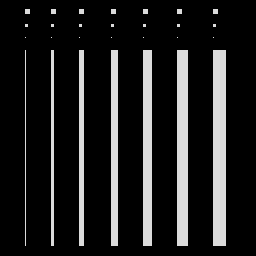
\includegraphics[width=.7\linewidth]{strips}
\caption{The \textit{strips} phantom}\label{Image:Strips}
\end{figure}

Figure~\ref{Image:Strips1LookExp} shows the result of adding single look noise in multiplicative fashion to the strips-and-dots image.
The background mean was set to $1$, and the rest to $5$.
The image is shown after equalization.

\begin{figure}[hbt]
	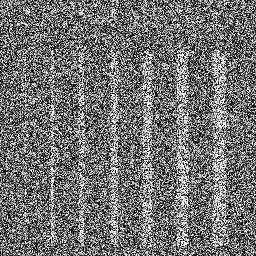
\includegraphics[width=.7\linewidth]{stripsExp1}
	\caption{The \textit{strips} phantom with exponential noise (after equalization)}\label{Image:Strips1LookExp}
\end{figure}

The effect of speckle is noticeable.
The small details, both the fine strip and the dots are now barely visible.

Figure~\ref{Plot:Transects} shows a horizontal and e vertical transect of both the phantom (in dark violet) and the observed (in violet) data.
The mean values ($5$ and $10$) are shown as dashed black lines.
This kind of representation is useful for checking the effect of filters around edges.

\begin{figure*}[hbt]
	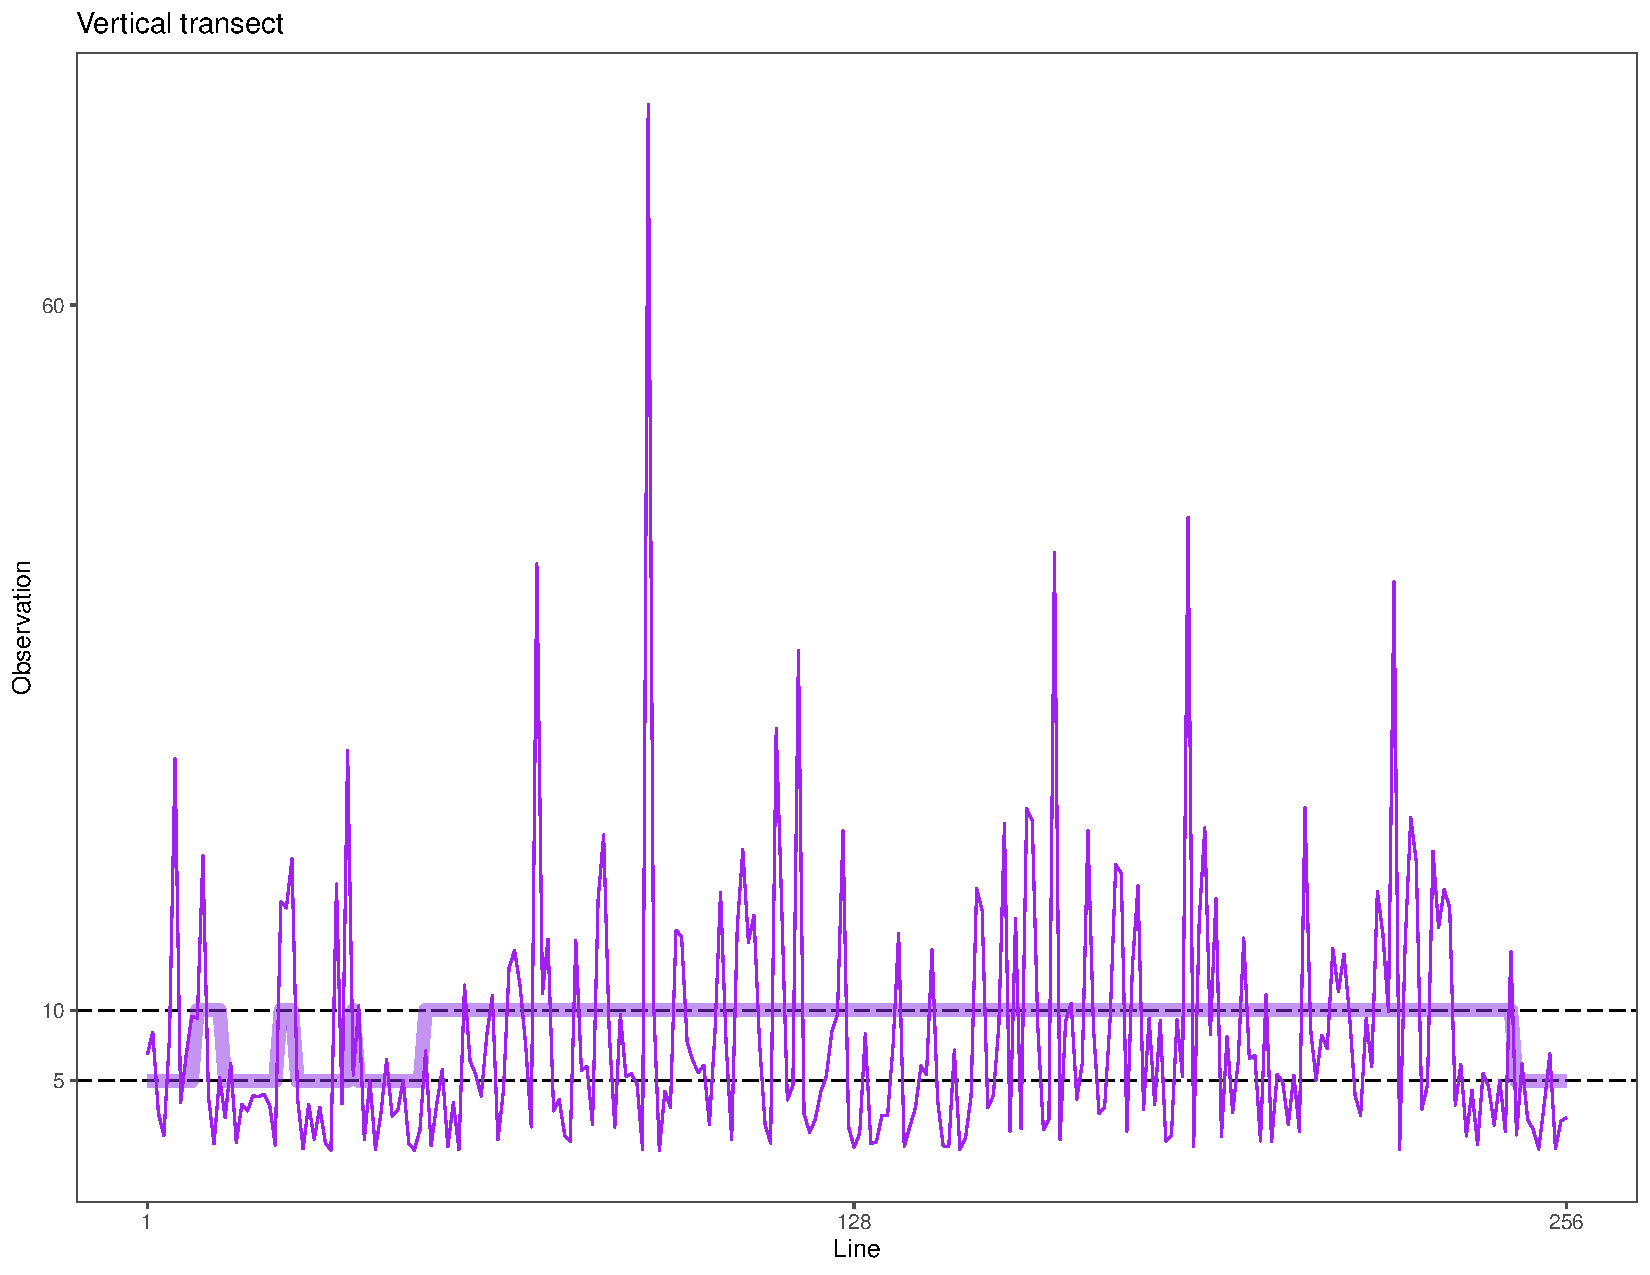
\includegraphics[width=.48\linewidth]{VerticalTransect}
	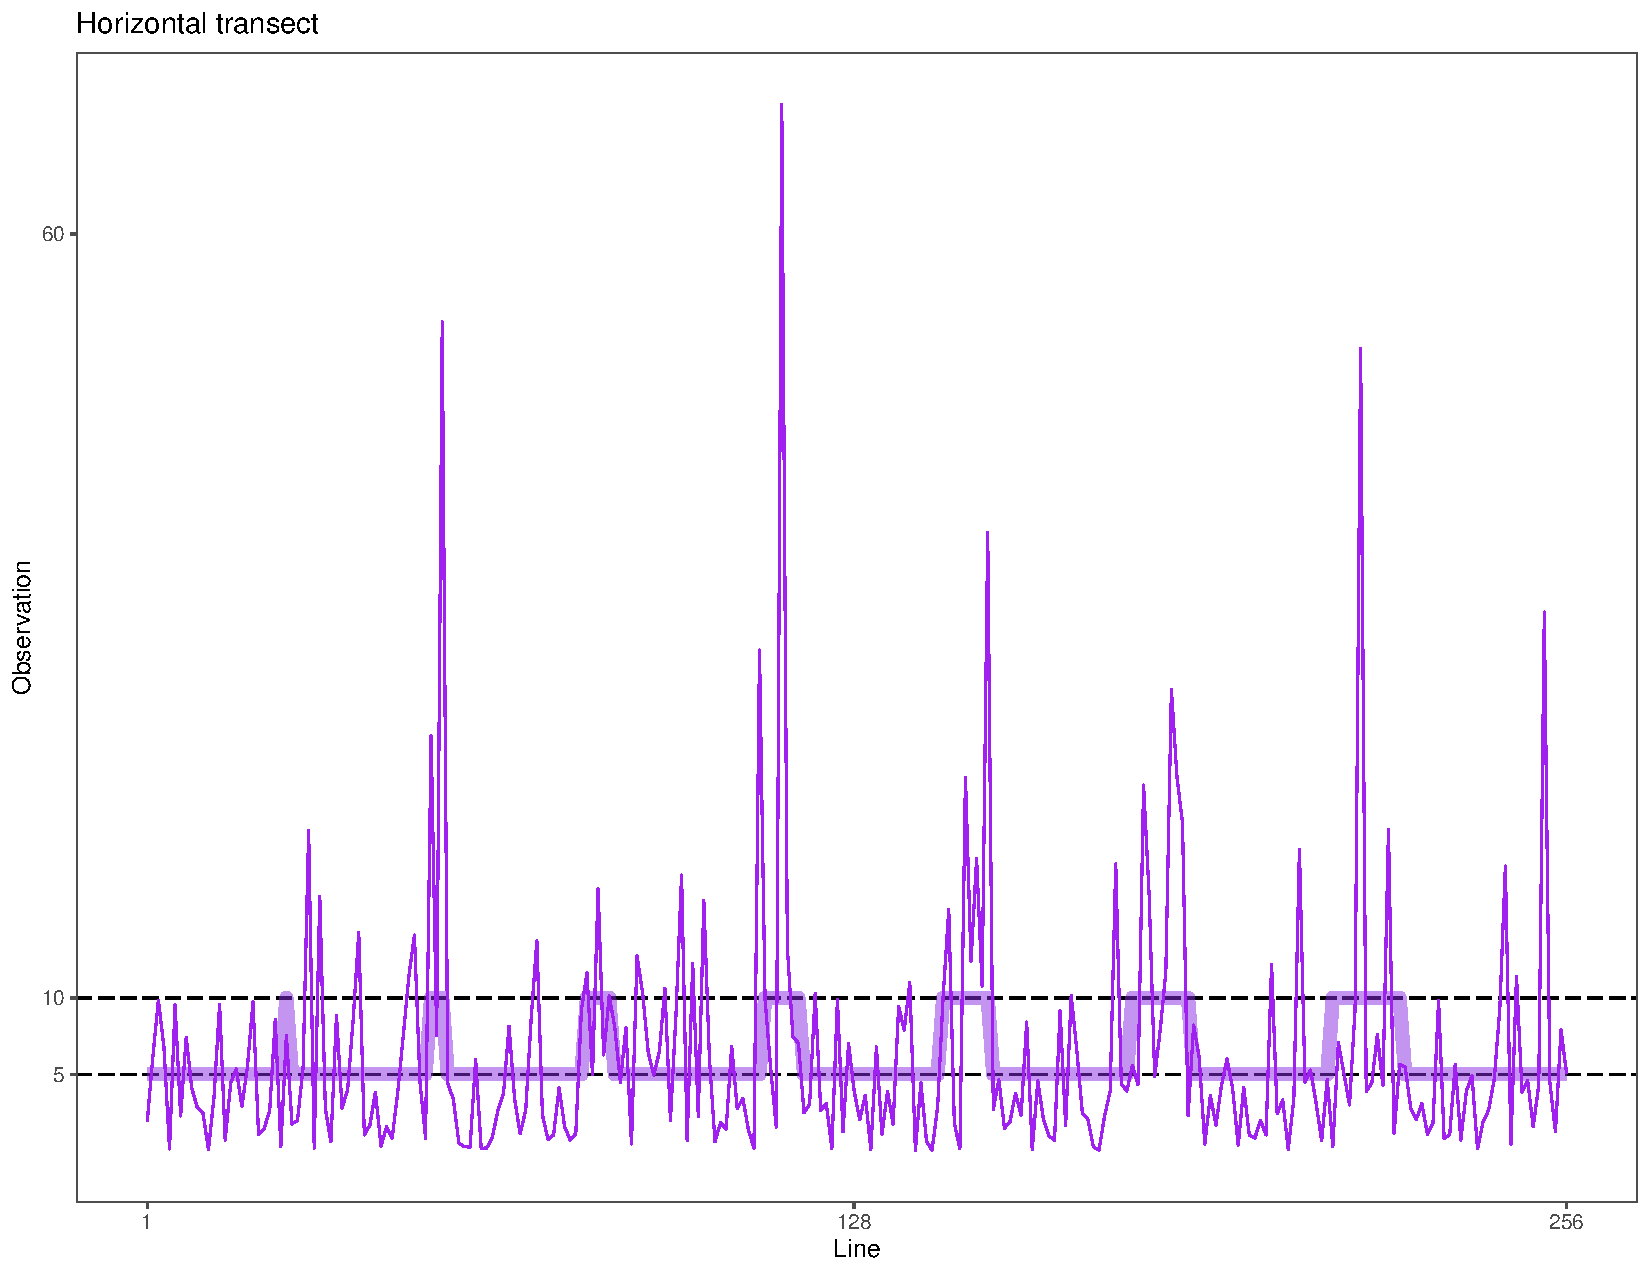
\includegraphics[width=.48\linewidth]{HorizontalTransect}
	\caption{Vertical (left) and horizontal (right) transects}\label{Plot:Transects}
\end{figure*}

Figure~\ref{Image:Exp1Mean} shows the results of applying the mean filter to the image shown in Fig.~\ref{Image:Strips1LookExp} with windows of sizes $3\times3$ and $15\times15$.
The noise in the new images has been reduced, but at the expense of blocking effect and loss of small details.

\begin{figure*}[hbt]
	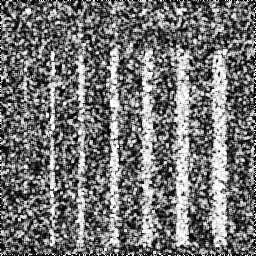
\includegraphics[width=.48\linewidth]{Exp1Mean3}
	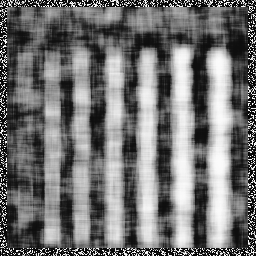
\includegraphics[width=.48\linewidth]{Exp1Mean15}
	\caption{Speckled strips filtered with the mean and windows of sizes $3\times3$ (left) and $15\times15$ (right)}\label{Image:Exp1Mean}
\end{figure*}

Figure~\ref{Image:Exp1Median} shows the results of applying the median filter to the image shown in Fig.~\ref{Image:Strips1LookExp} with windows of sizes $3\times3$ and $15\times15$.
The noise has also been reduced, also at the expense of blocking effect and loss of small details.

\begin{figure*}[hbt]
	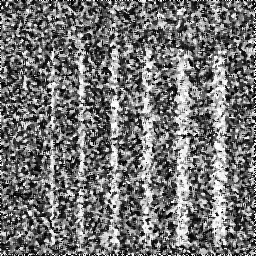
\includegraphics[width=.48\linewidth]{Exp1Median3}
	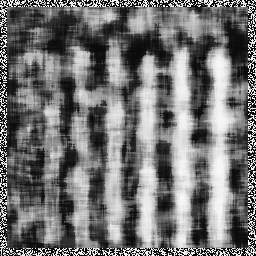
\includegraphics[width=.48\linewidth]{Exp1Median15}
	\caption{Speckled strips filtered with the median and windows of sizes $3\times3$ (left) and $15\times15$ (right)}\label{Image:Exp1Median}
\end{figure*}

The reader may notice that the blurring effect is smaller with the median than with the mean, mostly when applying the $15\times15$ window.
This desirable effect comes at a price: the noise is less reduced by the median than by the mean.

Figure~\ref{Image:TransectsFiltered} shows a horizontal transect after applying the mean and median filters of sizes $3\times3$ (left) and $15\times15$ (right).

\begin{figure*}[hbt]
	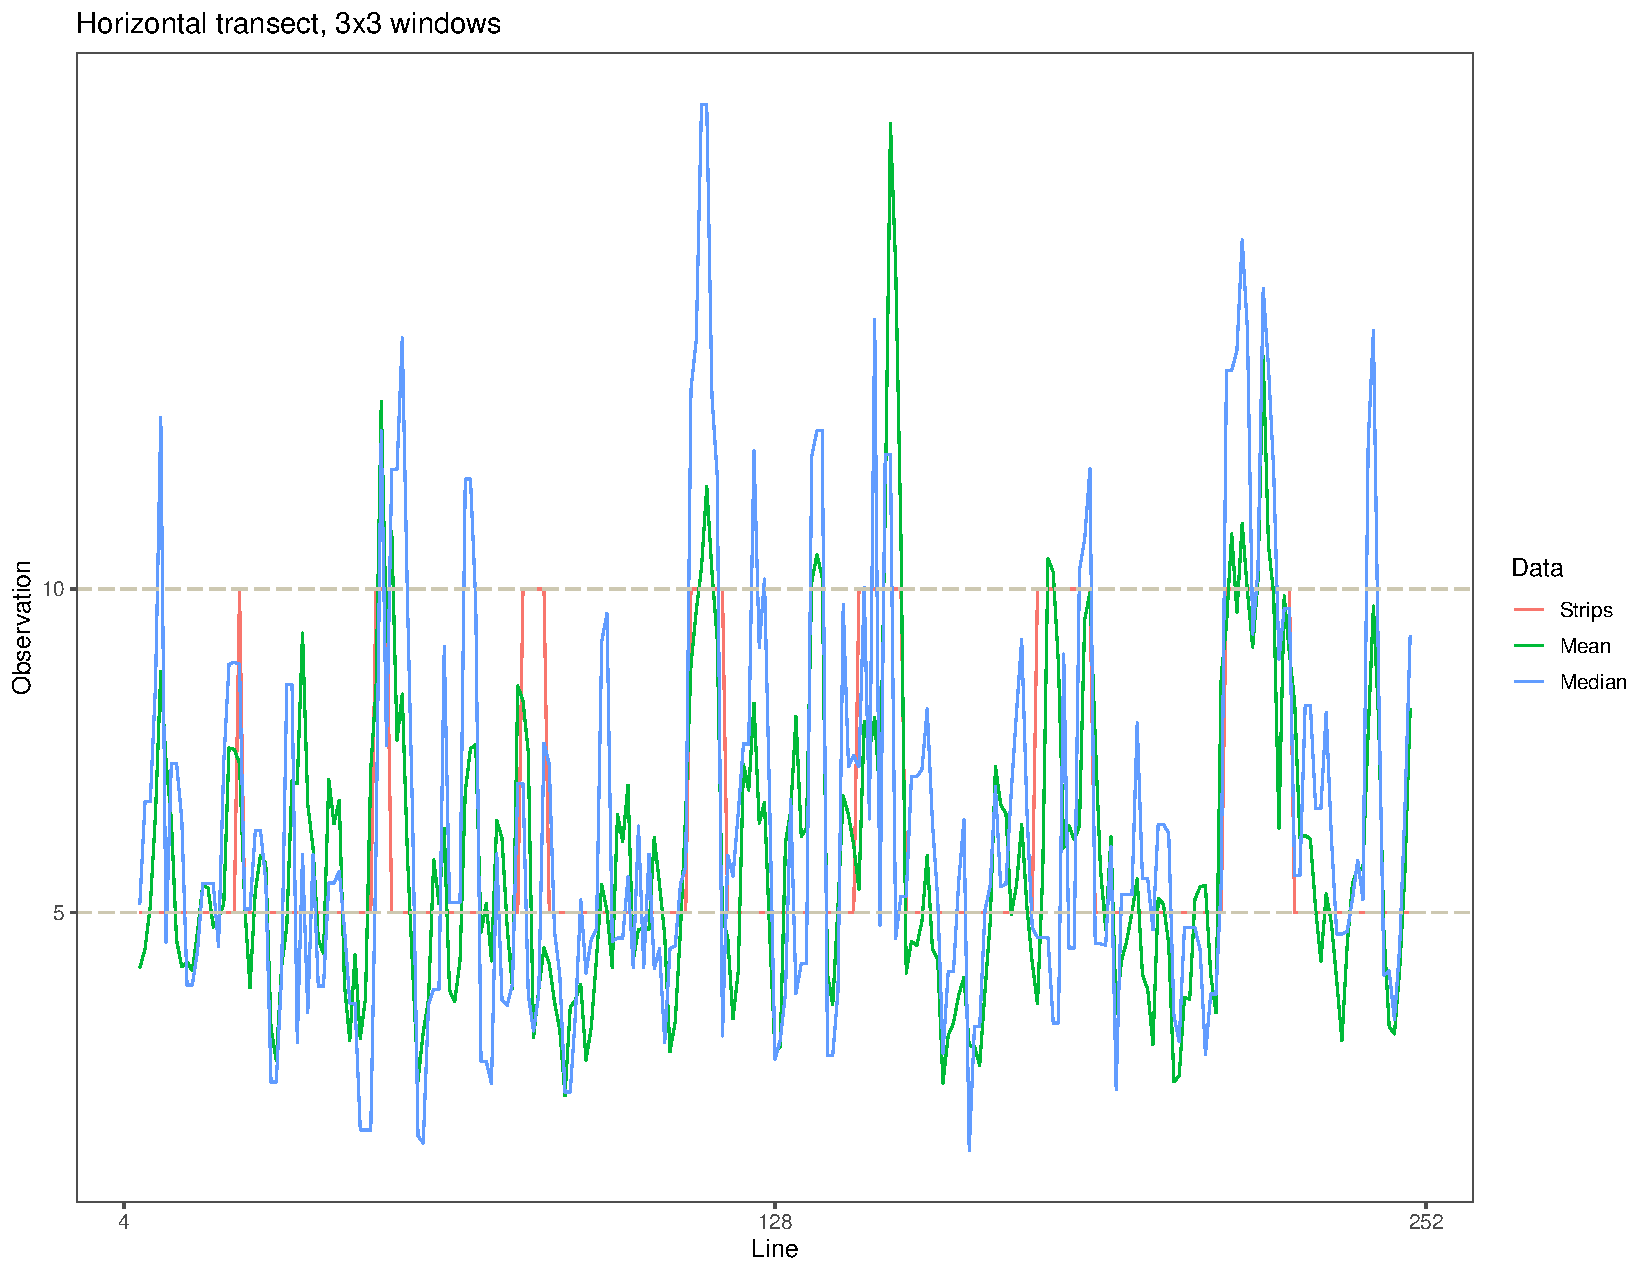
\includegraphics[width=.48\linewidth]{FilteredTransectMeanMedian3}
	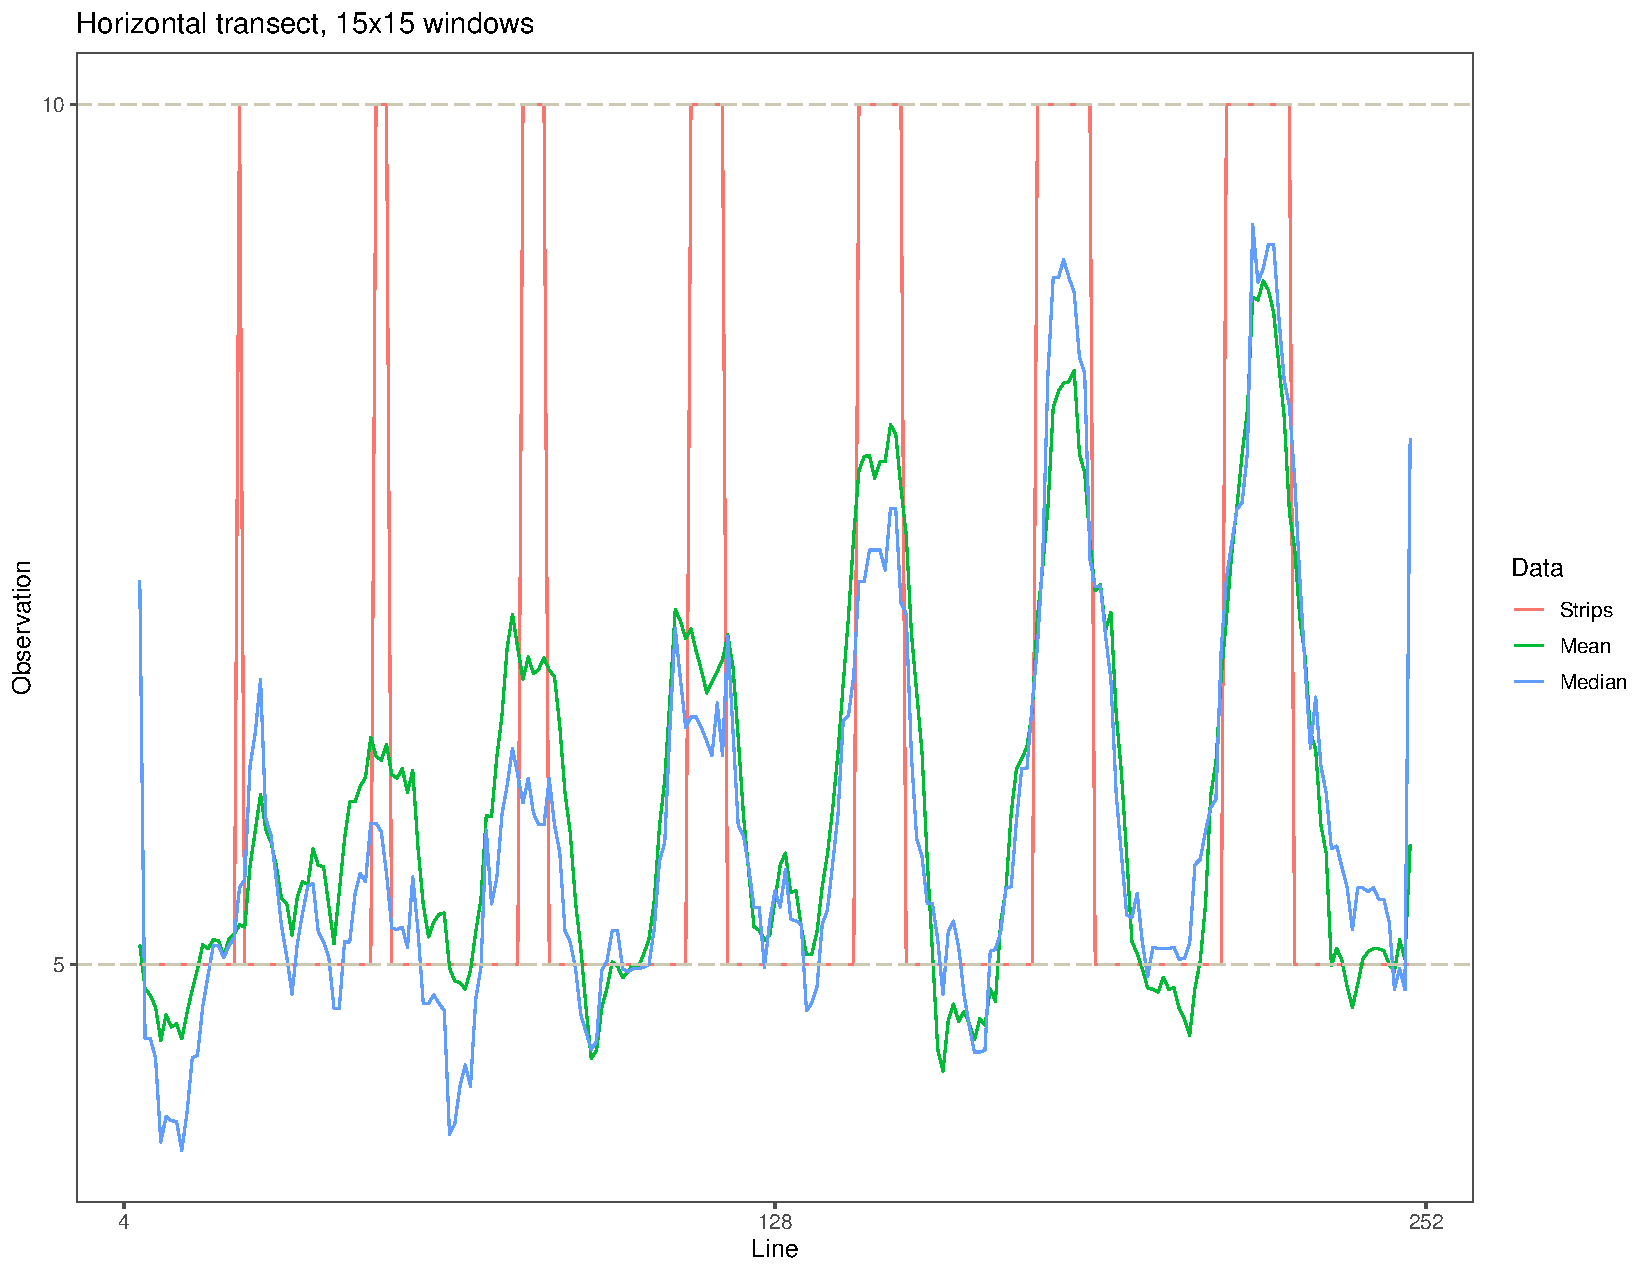
\includegraphics[width=.48\linewidth]{FilteredTransectMeanMedian15}
	\caption{Horizontal transect of the speckled strips filtered with the median and windows of sizes $3\times3$ (left) and $15\times15$ (right)}\label{Image:TransectsFiltered}
\end{figure*}
\chapter{Advanced Topics}\label{Chapter:AdvancedTopics}

\backmatter

%----------------------------------------------------------------------------------------
%	BIBLIOGRAPHY
%----------------------------------------------------------------------------------------

\bibliography{rdt,manuais,livros,art09,art11,art12,art17} % Use the bibliography.bib file for the bibliography
\bibliographystyle{plainnat} % Use the plainnat style of referencing

%----------------------------------------------------------------------------------------

\printindex % Print the index at the very end of the document

\end{document}